% !TeX encoding = UTF-8
% !TeX spellcheck = en_US
\documentclass[a4paper]{scrartcl}
%%%%%%%%%%%%%%%%%%%%%%%%%%%%%%%%%%%%%%%%%%%%%%%%%%%%%%%%%%%%%%%%%%%%%%%%%%%%%%%%%%%%%%%%%%%%%%%%%%%%%%%%%%%%%%%%%%%%%%%%%%%%%%%%%%%%%%%%%%%%%%%%%%%%%%%%%%%%%%%%%%%%%%%%%%%%%%%%%%%%%%%%%%%%%%%%%%%%%%%%%%%%%%%%%%%%%%%%%%%%%%%%%%%%%%%%%%%%%%%%%%%%%%%%%%%%


\usepackage[
nosolutionfiles %Lösungen werden direkt bei Aufgabe angezeigt, sonst in einer Datei gespeichert. Diese kann man auch unten einbinden
]{answers}
\newif\ifpartINTRO %\partINTROtrue
\newif\ifpartTSA   %\partTSAtrue
\newif\ifpartSVAR  %\partSVARtrue
\newif\ifpartDSGE  \partDSGEtrue
\newif\ifSolutEnd  %\partSolutEnd
\newcommand{\myTitle}{%Macroeconometrics:\\
					  %Univariate Time Series Analysis,\\
					  %(S)VAR 
					  %and
					  DSGE Models
				     }
%%%%%%%%%%%%%%%%%%%%%%%%%%%%%%%%%%%%%%%%%%%%%%%%%%%%%%%%%%%%%%%%%%%%%%%%%%%%%%%%%%%%%%%%%%%%%%%%%%%%%%%%%%%%%%%%%%%%%%%%%%%%%%%%%%%%%%%%%%%%%%%%%%%%%%%%%%%%%%%%%%%%%%%%%%%%%%%%%%%%%%%%%%%%%%%%%%%%%%%%%%%%%%%%%%%%%%%%%%%%%%%%%%%%%%%%%%%%%%%%%%%%%%%%%%%%
\Newassociation{solution}{Solution}{ans_macroeconometrics}
\usepackage[T1]{fontenc}
%\usepackage[utf8]{inputenc}
\usepackage[english]{babel}
\usepackage[bottom=2.5cm,top=2.0cm,left=2.0cm,right=2.0cm]{geometry}
\usepackage{amssymb,amsmath,amsfonts}
\usepackage{lmodern}
\usepackage{csquotes}
%\renewcommand{\labelenumi}{(\alph{enumi})}
%\renewcommand{\labelenumii}{(\roman{enumii})}
%\renewcommand{\Solutionlabel}[2]{\emph{Solution #1}}
%\renewenvironment{Solution}[1]{\begin{trivlist}\item
%		Solution to \emph{#1} }{\end{trivlist}}
%\renewcommand{\Solutionlabel}[1]{\emph{Solution to}}
%\renewcommand{\Solutionparams}{\Currentlabel \currentname (p.\thepage) }

%\parindent0mm
%\parskip1.5ex plus0.5ex minus0.5ex
%\renewcommand{\thesection}{{Aufgabe \arabic{section}:}}
%\renewcommand{\theenumi}{\alph{enumi}}
%\renewcommand\labelenumi{(\theenumi)}

\usepackage{graphicx}
\usepackage[usenames,dvipsnames]{color}
\definecolor{MyDarkGreen}{rgb}{0.0,0.4,0.0}
%\usepackage{listings}
\usepackage{listingsutf8}
\lstset{language=Matlab,                        % Use MATLAB
	frame=leftline,                           % Single frame around code
	basicstyle=\footnotesize\ttfamily,             % Use small true type font
	breaklines=false,                        %
	keywordstyle=[1]\color{Blue}\bfseries,  % MATLAB functions bold and blue
	keywordstyle=[2]\color{Purple},         % MATLAB function arguments purple
	keywordstyle=[3]\color{Blue}\underbar,  % User functions underlined and blue
	morekeywords={matlab2tikz},
	identifierstyle=,                       % Nothing special about identifiers
	commentstyle=\usefont{T1}{pcr}{m}{sl}\color{MyDarkGreen}\small, 	% Comments small dark green courier
	stringstyle=\color{Purple},             % Strings are purple
	showstringspaces=false,                 % Don't put marks in string spaces
	tabsize=3,                             % 5 spaces per tab
	%
	%%% Put standard MATLAB functions not included in the default
	%%% language here
	%morekeywords={xlim,ylim,var,alpha,factorial,poissrnd,normpdf,normcdf},
	%
	%%% Put MATLAB function parameters here
	%morekeywords=[2]{on, off, interp},
	%
	%%% Put user defined functions here
	%morekeywords=[3]{FindESS, homework_example},
	%
	morecomment=[l][\color{Blue}]{...},     % Line continuation (...) like blue comment
	numbers=left,                           % Line numbers on left
	firstnumber=1,                          % Line numbers start with line 1
	numberstyle=\tiny\color{Blue},          % Line numbers are blue
	stepnumber=5                            % Line numbers go in steps of 5
}
\usepackage{natbib}
\bibliographystyle{Chicago}
%\usepackage[notes,natbib,isbn=false,backend=biber]{biblatex-chicago}  
\usepackage[stable]{footmisc}
\usepackage{nameref}
%\makeatletter
%\newcommand*{\currentname}{\@currentlabelname}
%\makeatother
\usepackage[hidelinks]{hyperref} 
\begin{document}
	\title{\myTitle\\ -- Exercise And Solution Booklet --}
	\author{Willi Mutschler\\willi@mutschler.eu}
	\date{Version: \today}
	\maketitle\thispagestyle{empty}
	\newpage
	\Opensolutionfile{ans_macroeconometrics}[ans_macroeconometrics]
	\renewcommand{\contentsname}{Overview}
	\tableofcontents\thispagestyle{empty}\newpage

\ifpartINTRO	% if start for Introduction
\section[Macroeconometrics]{Macroeconometrics\footnote{Based on \cite{Schorfheide.2010} and \cite{FernandezVillaverdeRubioRamirez.2010}.}\label{ex:Macroeconometrics}}\setcounter{page}{1}
Broadly define the term and research topics of \enquote{Macroeconometrics}. How does the traditional (Cowles Commission) approach differ from the modern practice using structural vector autoregressive (SVAR) and dynamic stochastic general equilibrium (DSGE) models? What are the challenges in SVARs and DSGEs and their econometric evaluation?
\begin{solution}\textbf{Solution to \nameref{ex:Macroeconometrics}:}
\begin{itemize}
\item Definition of term: Combination of modern theoretical macroeconomics (the study of aggregated variables such as economic growth, unemployment and inflation by means of structural macroeconomic models) and econometric methods (the application of formal statistical methods in empirical economics).
\item Research topics:
\begin{itemize}
	\item How to identify sources of fluctuations, e.g. how important are monetary policy shocks as opposed to other shocks for movements in aggregate output? [forecast error variance decomposition]
	\item Understand propagation of shocks, e.g. what happens to aggregate hours worked over the next two years in response to a technology shock in the current quarter? [impulse response function]
	\item Forecasting the future, e.g. how will inflation and output growth rates evolve over next eight quarters. [forecasting]
	\item Predict effect of policy changes, e.g. how will output and inflation respond to an unanticipated change in nominal interest rate? [impulse response function and forecast scenarios]
	\item Structural changes in the economy, e.g. has monetary policy changed in the early 1980s, why did volatility of many macroeconomic time series drop in the mid 1980s, [historical decomposition]

	\item How much of the recession of 1982  would have deepened had monetary policymakers not responded to output growth at all. [policy counterfactual]
\end{itemize}
\item Traditional Cowles Commission approach: large-scale system-of-equations models developed from 1950s to 1970s. Came under attack in mid 1970s by (i) Lucas (1976) who argued that these models are unreliable tools for policy analysis because they are unable to predict effects of policy regime changes on the expectation formation of economic agents in a coherent manner $\rightarrow$ development of micro-founded dynamic stochastic general equilibrium (DSGE) models (RBC, new-Keynesian) and (ii) Sims (1980) who criticized that many restrictions that are used to identify behavioral equations in these models are inconsistent with dynamic macroeconomic theories $\rightarrow$ (structural) vector autoregressions ((S)VAR) as alternative.
\item SVAR approach: multivariate linear representation of a vector of observables on its own lags and (possibly) other variables as a trend or a constant. SVARs make explicit identifying assumptions to isolate estimates of policy and/or private agent's behavior and its effects on the economy while keeping the model free of many additional restrictive assumptions needed to give every parameter a behavioral interpretations. Identification restrictions, however, are dictated by the economic theory being studied.
\item DSGE approach: decision rules of economic agents are derived from assumptions about preferences and technologies by solving intertemporal optimization problems. Agents face uncertainty with respect to e.g. total factor productivity or nominal interest rate set by central bank. Uncertainty is generated by exogenous stochastic processes or shocks that shift technology or generate unanticipated deviations from a central bank's interest-rate feedback rule. Conditional on distributional assumptions for the exogenous shocks, the DSGE model generates a joint probability distribution for the endogenous model variables such as output, consumption, investment, and inflation.
\item Challenges in SVAR and DSGE: 
\begin{itemize}
	\item SVAR: many free parameters to estimate, need restrictions for e.g. good forecasts, difficult to predict effects of (rare) policy regime changes as expectation formation and behavior of economic agents are not explicitly modeled
	\item DSGE: trade-off between theoretical coherence and empirical fit
	\item Model specification: How to select the \enquote{right} model, how to cope with misspecification of SVARs and DSGE when taking them to data?
	\item Identification: parameters of a model are identifiable if no two parameterizations (or structures) of that model generate the same probability distribution for the observables. Problem of identification: flat likelihood estimation and inference not possible. In SVARs we need additional restrictions to identify structural, e.g. a monetary policy, shocks as the mapping between one-step-ahead forecast errors (residuals of reduced-form VAR) and the structural shocks is not unique. Do we want these restrictions to be compatible with a large class of models or find the one concrete and \enquote{correct} model? DSGE models can generate many parameter identification problems inherent in e.g. solution techniques as teh mapping from the structural parameters into the (approximated) solution parameters is highly nonlinear and typically can only be evaluated numerically.
	\item Macroeconomic time series are indicative of nonlinearities and time-varying volatility. In (S)VARs nonlinear dynamics are typically generated with time-varying coefficients, whereas most DSGE models are nonlinear and only for convenience approximated by linear rational expectations models. Implementation of computations is in both cases often cumbersome and challenging.
\end{itemize}

\end{itemize}
\newpage %for solutions at end
\end{solution}
\newpage
\fi  % if end for introduction

\ifpartTSA  %  if start for univatiate time series analysis


\section[Visualizing Time Series Data]{Visualizing Time Series Data\footnote{Based on \citet[Ch.~1]{BjornlandThorsrud.2015}.}}\label{ex:VisualizingTSData}
Analyze the quarterly growth rate of gross domestic product (GDP) in Norway. The data is given in the excel file \texttt{Quarterly\_GDP\_Norway.xlsx}. To this end, do the following:
\begin{itemize}
	\item Load the data. Save the dates and data in two variables. 
	\item Create a new figure and plot the data. Name it \enquote{Plot of data}.
	\item Create a new figure and plot a histogram with 10 bins. Call it \enquote{Histogram of data}. Compare it to a fitted normal distribution.
	\item Create a new figure and assess the fit to a normal distribution via a Q-Q plot. Call it \enquote{Normal probability plot}.
	\item Give a numerical estimator for the average growth rate and its standard deviation in the sample.
\end{itemize}
\begin{solution}\textbf{Solution to \nameref{ex:VisualizingTSData}}
\lstinputlisting{../progs/VisualizeData.m}
Remarks:
\begin{itemize}
\item A growth rate is usually approximated using logs $$\frac{Y_t - Y_{t-p}}{Y_{t-p}} \approx log \left(\frac{Y_t}{Y_{t-p}}\right)$$, where $p=1$ would correspond to one period lagged. For quarterly we would set $p=4$ or for monthly $p=12$.
\item Normal distribution is not a very bad choice, even though the normal plot suggests some curvature in tails of distribution.
\item There is roughly a 50 percent probability that GDP growth will be 0.6.
\end{itemize}
\newpage
\end{solution}

\newpage
\section[Definition and Frequencies of Time Series Data]{Definition and Frequencies of Time Series Data\footnote{Based on \citet[Ch.~2]{BjornlandThorsrud.2015}.}}\label{ex:DefFreqTS}
\begin{solution}\textbf{Solution to \nameref{ex:DefFreqTS}}
\end{solution}
\begin{enumerate}
	\item Briefly define a time series in terms of random variables and stochastic processes.	
	\begin{solution}
		A time series is a collection of observations $Y_t$ indexed by the date of each observation $t$. For simplicity often one denotes $t=0,1,2,...,T$, then $\{Y_t\}_0^T = \{Y_0,Y_1,Y_2,...,Y_T\}$ is a sequence of random variables ordered in time (each $Y_t$ is a random variable) which we call a stochastic process. Sometimes we rely on an infinite sample and consider $\{Y_t\}_{t=-\infty}^\infty$ or simply $\{Y_t\}$. A stochastic process can have many outcomes, due to its randomness, and a single outcome of a stochastic process is called a sample function or realization. A time series model assigns a joint probability distribution to the stochastic process.
	\end{solution}
	
	\item Consider figure \ref{fig:NorwayData} depicting various time series for Norway.
		\begin{figure}[h]
		\centering
		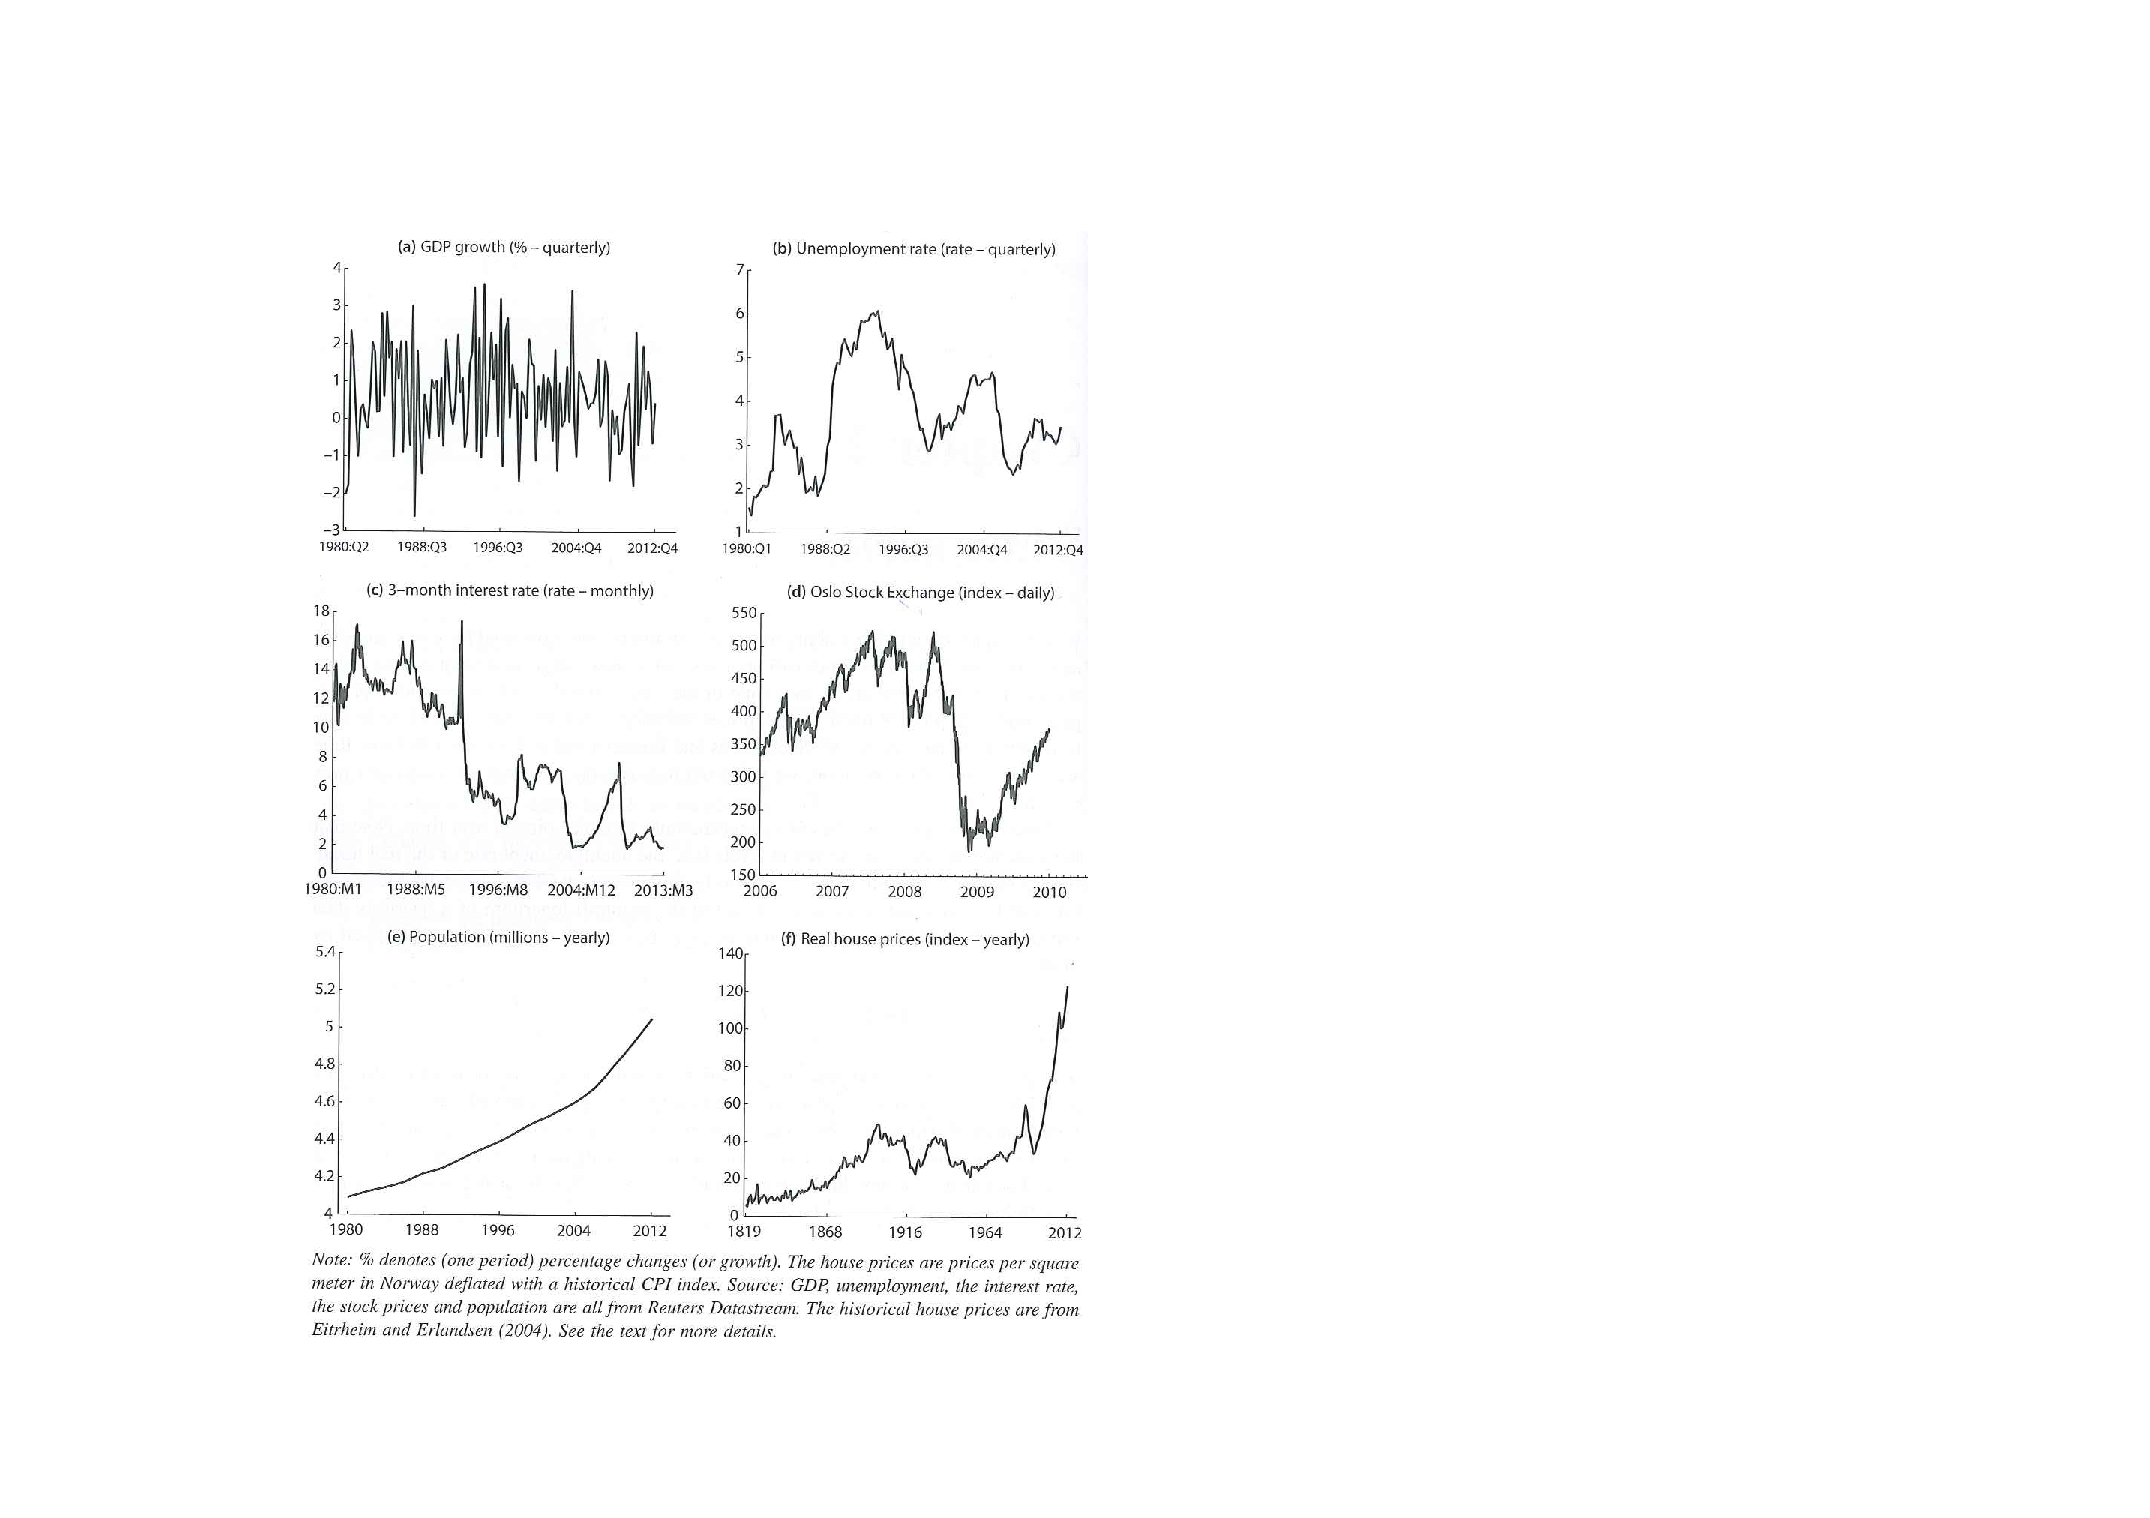
\includegraphics[width=0.6\linewidth]{NorwayDataOverview.pdf}
		\caption{Various Time Series For Norway}
		\label{fig:NorwayData}
		\end{figure}
	\begin{enumerate}
		\item What data frequencies do the individual plots have? For what type of economic analysis would you use these frequencies?
		\begin{solution}
			Variables are either measured in levels (unemployment rate, real house price index) or as growth rates (quarterly growth GDP).
			
			Wide range of frequencies:
			\begin{itemize}
				\item Daily data: Figure d
				\item Monthly data: Figure c
				\item Quarterly data: Figure a and b
				\item Yearly data: Figure e and f
			\end{itemize}
		For business cycle analysis one usually focuses on monthly and quarterly data; for understanding stock returns we consider daily or monthly data; for long-run growth and wealth of nations yearly data might be sufficient.
		
		Note: Aggregation of higher frequency to lower frequencies is straightforward (eg. take some mean or last value), for the other way around we need different tools, e.g. interpolation, spline functions etc. $\rightarrow$ not straightforward!
		\end{solution}
	
		\item What are the sample sizes? Is it always better to have a larger sample size from an economic and/or statistical point of view?
		\begin{solution}
			Sample sizes vary considerably. While quarterly data cover a much shorter sample than e.g. yearly house prices series, the number of observations are not that different (roughly 190 vs. 130 observations). Many results in statistics and econometrics depend on having many observations, so we could consider higher frequencies. But consider figure d: nearly 300 business day observations every year. However, information in all these daily data does not say much about, say, the overall state of the economy. We rather have three periods: 2006/07 when stock index hovered around 375, period from mid-2007 to mid-2008 when index fluctuated around 450 and the sharp fall during the financial crisis. From a macroeconomic perspective we rather have just three \enquote{informative} periods, all other observations are more or less just noise. So it is not always better to have a larger sample size if is uninformative.
		\end{solution}
	
		\item The logarithm of a given time series $\{Y_t\}$ can be thought of as the sum of four (additive) components:
		$$ \log{Y_t} =y_t = \underbrace{g_t}_\text{trend} + \underbrace{c_t}_\text{cycle} + \underbrace{s_t}_\text{season} + \underbrace{\varepsilon_t}_\text{noise}$$
		To what degree do you find these features in the figure? Intuitively what do we mean when we talk about stationary or non-stationary data?
		\begin{solution}
			Non-stationary: data trends upwards or downwards over time, e.g. population and house prices (figure e and f). Stationary: observations are moving randomly up and down around a more or less constant mean (e.g. GDP growth).
			
			Some figures have a pronounced cyclical pattern with longer positive or negative departures from a given mean value, e.g. unemployment.
		\end{solution}
		\item Consider the plots jointly. What are possible macroeconomic topics one could analyze?
		\begin{solution}
			Examining macroeconomic and financial data jointly (not just individually), we could analysis for instance:
			\begin{itemize}
				\item While financial crisis is clearly visible in the stock exchange, the effect on unemployment rate or real house prices is hard to detect. Real income, job opportunities and consumder confidence remained high. Why?
				\begin{itemize} 
					\item Maybe monetary policy influenced the behavior of the unemployment rate as Figure c indicates expansionary monetary policy. What is role of fiscal policy in the business cycle.
					\item Or Norwegian oil sector is highly productive (makes up 25\% of GDP) so thats the reason why the crisis was cushioned.
				\end{itemize}
				\item Are house prices in line with their fundamentals? Is there a bubble?
			\end{itemize}
		\newpage
		\end{solution}
	\end{enumerate}
	
\end{enumerate}
\newpage

\section[Some Fundamental Concepts Of Univariate Time Series Analysis]{Some Fundamental Concepts Of Univariate Time Series Analysis\footnote{Based on \citet[Ch.~2]{BjornlandThorsrud.2015}.}}\label{ex:FundamentalConceptsUnivariateTSA}
Three important fundamental concepts when using time series models are the white-noise process, stationarity and lag-operator.
\begin{solution}\textbf{Solution to \nameref{ex:FundamentalConceptsUnivariateTSA}}
\end{solution}

\begin{enumerate}
	\item Define a White Noise process $WN(0,\sigma_\varepsilon^2)$. Plot 200 observations of 
	\begin{align*} (i)~y_t&=\varepsilon_t\\ (ii)~y_t &= \frac{1}{5}(\varepsilon_{t-2}+\varepsilon_{t-1}+\varepsilon_{t}+\varepsilon_{t+1}+\varepsilon_{t+2})
	\end{align*} with $\varepsilon_{t} \sim N(0,1)$. What are the differences?
	\begin{solution}
		A white noise has mean zero and constant variance $\sigma^2$, whereas all other autocovariances are zero, i.e. $Cov(\varepsilon_{t},\varepsilon_s) = E(\varepsilon_t \varepsilon_s) - E(\varepsilon_t)E(\varepsilon_s) = E(\varepsilon_t \varepsilon_s) = 0$ for $s \neq t$.		
		\lstinputlisting{../progs/WhiteNoisePlots.m}
		Every simulation is different, model can thus generate an infinite set of realizations over the period $t=1,...,200$. 
		
		(i) is a white noise process, it is not persistent.		
		(ii), the 5-point-moving-average is more in line with real observations, as it is a linear combination of white noise processes. It is smoother and more persistent and very different from just noise. Linear combinations of white noise processes build the fundament of many models in time series analysis.
	\end{solution}

	\item Briefly explain the concepts of weak and strict stationarity. Define the autocovariance and autocorrelation function for a stationary stochastic process $\{Y_t\}$.
	\begin{solution}
	Weak stationarity or covariance stationarity: $E(Y_t)=\mu$ (usually $\mu=0$), $var(Y_t)=E(Y_t - \mu)(Y_t-\mu)=\sigma_Y^2$ for all $t$ and $E(Y_t-\mu)(Y_s-\mu)=E(Y_t-\mu)(Y_{t-|t-s|}-\mu)=0$ for $t\neq s$, i.e. no autocorrelation.\\
	Strict stationarity: for all $m$ and $h$ $$f(Y_t,Y_{t-1},...,Y_{t-m})=f(Y_{t-h},Y_{t-h-1},...,Y_{t-h-m})$$
	Autocovariance function for a stationary process: $$\gamma_k = E(Y_t - \mu)(Y_{t-k}-\mu)$$ where $\gamma_0$ is the variance. Autocorrelation function: $$\rho_k = \gamma_k/\gamma_0$$ How to estimate:
	\begin{align*}
	\hat{\gamma}_k = c_k &= \frac{1}{T} \sum_{y_t -\bar{y}}(y_{t-k}-\bar{y})\\
	\hat{\rho}_k = r_k & = c_k/c_0
	\end{align*}
	Note: Degrees of freedom are sometimes corrected by the observations needed to estimate the parameters of the model.
	\end{solution}
	
	\item Consider the linear first-order difference equation $$y_t=\phi y_{t-1}+\varepsilon_t$$ Simulate and plot 200 observations of (i) $|\phi|<1$, (ii) $\phi=1$ and (iii) $|\phi| >1$. What does this suggest in terms of stationarity?
	\begin{solution}~		
		\lstinputlisting{../progs/ARPlots.m}
	Remarks: If $|\phi|<1$ the series returns to the mean, i.e. it is stable and stationary. If $|\phi>1|$ then it explodes, i.e. it is unstable and not stationary. $\phi=1$ is a so-called random walk, it is the key model when working with non-stationary models. Note that the random walk incorporates many different shapes, in macroeconomic forecasts we often want to \enquote{beat} the random walk model.
	\end{solution}
	\item Briefly explain the Lag-operator and Lag-polynomials. How do you check stationarity?
	\begin{solution}
		It is a special LINEAR operator, similar to the expectation operator, and very useful when working with time series. The operator transforms one time series into another by shifting the observation from period $t$ to period $t-1$: $Ly_t = y_{t-1}$ or $L^{-1} y_t =y_{t+1}$. More general: $L^k y_t = L^{k-1} L y_t = L^{k-1} y_{t-1} = ... = y_{t-k}$. Convenient use:
		$$(1-L)y_t = y_t - y_{t-1}= \Delta y_t$$
		
		We can also work with lag-polynomials:$$ \phi(L) = (1-\phi_1 L-\phi_2 L^2 -... - \phi_p L^p)$$ where we call p the lag order. So:
		$$ \phi(L) y_t = (1-\phi_1 L-\phi_2 L^2 -... - \phi_p L^p)y_t = y_t - \phi_1 y_{t-1} -\phi_2 y_{t-2} - ... - \phi_p y_{t-p}$$
		For stationarity: check whether the roots of the lag-polynomial (treat $L$ as a complex number $z$) lie outside the unit circle.
		\newpage
	\end{solution}
\end{enumerate}
\newpage

\section[Properties of AR(1)]{Properties Of AR(1)\footnote{Based on \citet[Ch.~2]{BjornlandThorsrud.2015} and \citet{Luetkepohl.2004}.}}\label{ex:PropertiesAR1}
Let $\{\varepsilon_t\}$ be a white noise process.
\begin{solution}\textbf{Solution to \nameref{ex:PropertiesAR1}}
\end{solution}
\begin{enumerate}
	\item Consider the first-order autoregressive, i.e. AR(1), model:  $$y_t = \phi y_{t-1} + \varepsilon_{t}$$ Derive the conditional and unconditional first and second moments.
	\begin{solution}
		\begin{itemize}
			\item Recursive substitution (starting at some infinite time $j$):
			\begin{align*}
			y_t &= \phi y_{t-1} + \varepsilon_t\\
			&= \phi \left( \phi y_{t-2} + \varepsilon_{t-1}\right) + \varepsilon_t\\ 
			&= \phi^2(\phi y_{t-3} + \varepsilon_{t-2} ) + \phi \varepsilon_{t-1} + \varepsilon_t\\
			&\vdots\\
			& = \phi^{j+1} y_{t-{j+1}}+\phi^j \varepsilon_{t-j}+...+\phi^2 \varepsilon_{t-2} + \phi \varepsilon_t + \varepsilon_t
			\end{align*}
			$y_t$ is a linear function of an initial value and historical values of white noise. If $|\phi|<1$ and j becomes large, then $ \phi^{j+1} y_{t-{j+1}} \rightarrow 0$, thus we get a so-called $MA(\infty)$ process:
			$$y_t = \varepsilon_t + \phi \varepsilon_{t-1} + \phi^2 \varepsilon_{t-2}+... = \sum_{j=0}^\infty \phi^j \varepsilon_{t-j}$$
			\item With Lag Operators: works only if $|\phi| < 1$ and $\{y_t\}$ is bounded, that is, there exists a finite number $k$ such that $|y_t| < k$ for all t. Then
			\begin{align*}
			(1-\phi L) y_t = \varepsilon_t\\
			(1-\phi L)^{-1}(1-\phi L) y_t =	y_t = (1-\phi L)^{-1}\varepsilon_t\\
			\end{align*}
			We can use the geometric rule: $(1-\phi L)^{-1} = \lim\limits_{j\rightarrow \infty}(1+\phi L + \phi^2 L^2+...+(\phi L)^j)$
			Therefore:$$y_t = \varepsilon_t + \phi \varepsilon_{t-1} + \phi^2 \varepsilon_{t-2}+... = \sum_{j=0}^\infty \phi^j \varepsilon_{t-j}$$	
			
		\end{itemize}
		If we can express an AR process as a MA process, we call this process invertible.\\
		Unconditional Moments:
		\begin{align*}
			E(y_t) &= 0\\
			var(y_t) &= \frac{\sigma^2}{1-\phi}\\
			cov(y_t,y_{t-j}) &= \phi^j var(y_t) \text{ for } j>0
		\end{align*}
		Conditional Moments, conditional on $y_{t-1}$:
		\begin{align*}
		E(y_t|y_{t-1}) &= \phi y_{t-1}\\
		var(y_t|y_{t-1}) &= \sigma^2\\
		cov((y_t|y_{t-1}),(y_{t-j}|y_{t-j-1})) &= 0 \text{ for } j>0
		\end{align*}
		Conditional Moments, conditional on $y_{t-2}$:
		\begin{align*}
		E(y_t|y_{t-2}) &= \phi^2 y_{t-2}\\
		var(y_t|y_{t-2}) &= (1+\phi^2)\sigma^2\\
		cov((y_t|y_{t-2}),(y_{t-j}|y_{t-j-2})) &= \phi\sigma^2 \text{ for } j=1\\
		cov((y_t|y_{t-2}),(y_{t-j}|y_{t-2})) &= 0 \text{ for } j>1
		\end{align*}
		
	\end{solution}
	\item  Simulate different AR(1) processes and plot the corresponding autocorrelation function (ACF). To this end write a function \texttt{ACFPlots($y$,$p^{max}$,$\alpha$)} to plot the ACF of the data vector $y$ with maximum number of lags $p^{max}$. Also include an approximate (1-$\alpha$)\% confidence interval around zero in your plot. Hints: 
		 \begin{itemize}
		 	\item The empirical autocorrelation function at lag $k$ is defined as $r_k = c_k/c_0$ where
			$$c_k = \frac{1}{T} \sum_{t=k+1}^T (y_t - \bar{y})(y_{t-k}-\bar{y})$$ and $$c_0 = \frac{1}{T} \sum_{t=1}^T (y_t - \bar{y})(y_{t}-\bar{y})$$
			You can either use a for-loop to compute the sum or use vectors: $(y - \bar{y})'(y - \bar{y})$.
		 	\item The sample autocorrelations are estimates of the actual autocorrelations if the process is stationary. If it is purely random, that is, all members are mutually independent and identically distributed so that $y_t$  and $y_{t-k}$ are stochastically independent for $k\neq 0$, then the normalized estimated autocorrelations are asymptotically standard normally distributed, i.e. $\sqrt{T} r_k \rightarrow U \sim N(0,1)$ and thus $r_k \rightarrow \tilde{U} \sim N(0,1/T)$. 
		 \end{itemize}
	
	 \begin{solution}
		 The ACF is a useful plot to understand the dynamics of a process:
		 \lstinputlisting{../progs/ACFPlots.m}
		 \newpage
	 \end{solution}
\end{enumerate}
\newpage

\section[AR(1) With Time Trend]{AR(1) With Time Trend}\label{ex:AR1timetrend}
Consider the AR(1) model with constant and time trend
$$ y_t = c + d\cdot t + \phi y_{t-1} + u_t$$
where $u_t \sim iid(0,\sigma^2)$, $|\phi|<1$, $c \in \mathbb{R}$ and $d \in \mathbb{R}$.
\begin{solution}\textbf{Solution to \nameref{ex:AR1timetrend}}\end{solution}
\begin{enumerate}
	\item Compute the unconditional first and second moments, i.e. the unconditional mean, variance, autocovariance and autocorrelation of $y_t$.
	\begin{solution}		
		\begin{align*}
			y_t &= c + d\cdot t + \phi y_{t-1} + u_t\\
			\Leftrightarrow y_t &= \frac{c + d\cdot t + u_t}{1-\phi L}\\
			\Leftrightarrow y_t &= \sum_{j=0}^{\infty}\phi^j(c+d(t-j)+u_{t-j}) = \frac{c}{1-\phi} + \frac{dt}{1-\phi} - d\sum_{j=0}^{\infty}\phi^j j + \sum_{j=0}^{\infty}\phi^j u_{t-j}
		\end{align*}
		as $|\phi| <1$ the geometric series holds. For $\sum_{j=0}^{k} \phi^j j$ we also have a closed-form formula, which can be derived similar to the geometric series:
		\begin{eqnarray*}
			\text{Denote } S_{k}  
			&=&	\sum_{j=0}^{k} \phi^j j = \sum_{j=1}^{k} \phi^j j
			=	\phi^1 \cdot 1 + \phi^2 \cdot 2+ \phi^3 \cdot 3 + \dots +  	
			\phi^k \cdot k, \\
			\text{then } \phi S_{k} 
			&=& \phi^2 \cdot 1 + \phi^3 \cdot 2+ \phi^4 \cdot 3 + \dots +  	
			\phi^{k+1} \cdot k \\
			\text{and we get } (1 - \phi) S_{k}
			&=& \phi^1 \cdot 1+ \phi^2 \cdot 1 + \phi^3 \cdot 1 + \dots + \phi^{k} \cdot 1 - \phi^{k+1} \cdot k \\
			S_{k}	&=& \frac{1}{1 - \phi} \sum_{j = 1}^{k} \phi^j - \frac{\phi^{k+1}}{1 - \phi} k.
		\end{eqnarray*} 
		Looking at the limit of $S_{k}$ for $k \to \infty$, we get
		$\lim\limits_{k \to \infty} S_{k} = \frac{\phi}{(1 - \phi)^2}$. \\
		Therefore, $y_{t}$ is given by
		\begin{displaymath}
		y_{t} = \frac{c}{1-\phi} + \frac{dt}{1-\phi} - d \frac{\phi}{(1 - \phi)^2}  + \sum_{j=0}^{\infty} \phi^j u_{t-j}.
		\end{displaymath} 
		
		Unconditional mean:
		\begin{eqnarray*}
			E[y_{t}] &=& \frac{c}{1-\phi} + \frac{dt}{1-\phi} - d \frac{\phi}{(1 - \phi)^2}  + \underbrace{\sum_{j=0}^{\infty} \phi^j E[u_{t-j}]}_{=0 \text{, as } \space  u_{t} \sim iid(0, \sigma^2)} \\
			&=& \frac{c}{1-\phi} + \frac{dt}{1-\phi} - d \frac{\phi}{(1 - \phi)^2}
		\end{eqnarray*}	
	
		Unconditional variance:
		\begin{eqnarray*}
			Var[y_{t}] 
			&=& E[(y_{t} - E[y_{t}])^2 ] \\
			&=& E[(\sum_{j=0}^{\infty} \phi^j E[u_{t-j}]) \cdot (\sum_{j=0}^{\infty} \phi^j E[u_{t-j}])] \\
			&=& E[(u_{t} + \phi^1 u_{t-1} + \phi^2 u_{t-2} + \dots)(u_{t} + \phi^1 u_{t-1} + \phi^2 u_{t-2} + \dots)] \\
			&=& E[	u_{t}^2 + 2\phi^1 u_{t}u_{t-1} + 2\phi^2 u_{t}u_{t-2} + \dots + 
			\phi^2 u_{t-1}^2 + 2\phi^3 u_{t-1}u_{t-2} + 2\phi^4 u_{t-1}u_{t-3} + \dots  \\
			&&+ \phi^4 u_{t-2}^2 + 2\phi^5 u_{t-2}u_{t-3} + 2\phi^5 u_{t-2}u_{t-4} + \dots ] \\
			&\overset{iid}{=}& E [ u_{t}^2+ \phi^2 u_{t-1}^2 + \phi^4 u_{t-2}^2 + \dots ] \\
		\end{eqnarray*}
		$\text{with } Var[u_{t}] = E[u_{t}^2] - E[u_{t}]^2 = E[u_{t}^2] = \sigma^2 \text{ we get}$
		\begin{displaymath}
		Var[y_{t}] = \sigma^2 ( \phi^0 + \phi^2 + \phi^4 + \dots )] = \frac{\sigma^2}{1-\phi^2}.
		\end{displaymath}
	
		Autocovariance: $\gamma(h)  = Cov(y_{t}, y_{t-h})$ for $|h| = k$ 
			\begin{eqnarray*}
				\gamma(k)
				&=& E[(y_{t}-E[y_{t}])(y_{t-k}-E[y_{t-k}])] \\
				&=& E[(\sum_{j=0}^{\infty} \phi^j 
				u_{t-j})(\sum_{j=0}^{\infty} \phi^j u_{t-j-k})] \\
				&=& E[(u_{t} + \phi^1 u_{t-1} + \phi^2 u_{t-2} + \dots + 
				\phi^k u_{t-k}  + \phi^{k+1} u_{t-k-1} + \phi^{k+2} u_{t-k-2} + \dots) \\
				&& 	(u_{t-k}  + \phi^{1} u_{t-k-1} + \phi^{2} u_{t-k-2} + \dots)] \\
				&=& E[u_{t}u_{t-k} + \phi^1 u_{t} u_{t-k-1} + \phi^2 u_{t} 
				u_{t-k-3} + \dots   \\
				&&	\phi^1 u_{t-1}u_{t-k} + \phi^2 u_{t-1}u_{t-k-1}	+ \phi^3 
				u_{t-1}u_{t-k-2} + \dots \\
				&& 	\phi^2 u_{t-2}u_{t-k} + \phi^3 u_{t-2}u_{t-k-1}	+ 
				\phi^4 u_{t-2}u_{t-k-2} + \dots \\
				&&	\vdots \\
				&&  \phi^{k} u_{t-k}^2 + 2\phi^{k+1} u_{t-k}u_{t-k-1}	+ 	
				2\phi^{k+2} u_{t-k}u_{t-k-2} + \dots \\
				&& 	\phi^{k+2} u_{t-k-1}^2 + 2\phi^{k+3} u_{t-k-1}u_{t-k-2} +
				2\phi^{k+4} u_{t-k-1}u_{t-k-3} + \dots \\ 
				&& 	\phi^{k+4} u_{t-k-2}^2 + 2\phi^{k+5} u_{t-k-2}u_{t-k-3} +
				2\phi^{k+6} u_{t-k-2}u_{t-k-4} + \dots] \\
				&\overset{iid}{=}& 
				E[\phi^{k}u_{t-k}^2 + \phi^{k+2}u_{t-k-1}^2 + \phi^{k+4}u_{t-k-2}^2 + \dots] \\
				&=& \phi^{k}\sigma^2(\phi^0 + \phi^2 + \phi^4 + \dots ) \\
				&=& \frac{\phi^{k}\sigma^2}{1-\phi^2}
			\end{eqnarray*}

		Autocorrelation: $\rho(h)  = \frac{\gamma(h)}{\gamma(0)}$. Therefore:
			\begin{displaymath}
			\rho(k) = \frac{\gamma(k)}{\gamma(0)} = \frac{\frac{\phi^{k}\sigma^2}{1-\phi^2}}{\frac{\sigma^2}{1-\phi^2}} = \phi^{k}.
			\end{displaymath} 

	
	\end{solution}
	\item Why is this process not covariance-stationary? How could one proceed to make it covariance-stationary?
	\begin{solution}
		The expectation is time-dependent, hence it is not stationary. One could subtract the expectation, e.g. look at $y_{t}^{s} = y_{t} -E(y_t)$, where $y_t^s$ is now covariance stationary. The unknown coefficient$d$ may be estimated via e.g. OLS. first.
\newpage %for solutions at end
	\end{solution}
\end{enumerate}

\newpage

\section[Law Of Large Numbers]{Law Of Large Numbers}\label{ex:LLN}
Let $Y_{1},Y_{2},\ldots $ be an i.i.d. sequence of arbitrarily distributed random variables with finite variance $\sigma_Y ^{2}$ and expectation $\mu$. Define the sequence of
random variables
\begin{equation*}
\overline{Y}_{T}=\frac{1}{T}\sum_{t=1}^{T}Y_{t}
\end{equation*}
\begin{solution}\textbf{Solution to \nameref{ex:LLN}}\end{solution}
\begin{enumerate}
	\item Briefly outline the intuition behind the \enquote{law of large numbers}.
	\begin{solution}
		In probability theory, the law of large numbers (LLN) is a theorem that describes the result of performing the same experiment a large number of times (repetitions, trials, experiments, or iterations). According to the LLN, the average of the results obtained from a large number of trials should be close to the expected value, and will tend to become closer as more trials are performed. The laws of large numbers are the cornerstones of asymptotic theory. In this exercise, the LLN is about determining what happens to $\overline{Y}_T$ as $T\rightarrow\infty$ (note that $\overline{Y}_T$ is a random variable). The LLN states that this series converges to the expected value $\mu$. More precisely, the strong LLN implies that at the limit, we can exactly determine $\mu$. The weak LLN implies that we can only approximately determine $\mu$, even though we can make the approximation very very very close to $\mu$. This implies: 
		\begin{itemize}
			\item Strong LLN means almost-sure convergence: At some point adding more observation does not matter at all for the average, it would be exactly equal to the expected value. That is, the sequence $\overline{Y}_{1},\overline{Y}_{2},\ldots $ of random variables converges \textbf{almost surely} to a variable $\mu$, if
			\begin{equation*}
			Pr\left( \left\{ \lim_{T\rightarrow \infty }\overline{Y}_{T}=\mu\right\} \right) =1
			\end{equation*}
			or simply:
			\begin{equation*}
			\overline{Y}_{T}\overset{a.s.}{\rightarrow }\mu
			\end{equation*}
			This definition of convergence is not very important in econometrics.
			
			\item Weak LLN means that the sample mean converges in probability to the population mean. That is, the sequence $\overline{Y}_{1},\overline{Y}_{2},\ldots $ of random variables converges \textbf{in probability} to a variable $\mu$, if
			\begin{equation*}
			\lim_{T\rightarrow \infty }Pr\left( |Y_{T}-\mu|<\delta \right) =1
			\end{equation*}
			The probability is approaching 1 as $T\rightarrow \infty$ very closely, but not actually 1. In other words, the probability that the average is \enquote{far} (more than an arbitrary small number $\delta$) from the expectation $\mu$ is zero. More compactly:
			\begin{eqnarray*}
				\overline{Y}_{T} &\overset{p}{\rightarrow }&\mu \\
				\textsl{plim}~\overline{Y}_{T} &=&\mu
			\end{eqnarray*}
			This definition of convergence is very important in econometrics. There are different necessary and sufficient conditions depending on the process at study.
		\end{itemize}		

	\end{solution}
	\item Write a program to illustrate the law of large numbers for uniformly $(u)$ distributed random variables (you may also try different distributions such as normal, gamma, geometric, student's t with finite or infinite variance). To this end, do the following:
	\begin{itemize}
		\item Set $T=10000$ and initialize the $T \times 1$ output vector $u$.
		\item Choose values for the parameters of the uniform distribution. Note that $E(u) = (a+b)/2$, where $a$ is the lower and $b$ the upper bound of the uniform distribution.
		\item For $t=1,...,T$ do the following computations:
		\begin{itemize}
			\item Draw $t$ random variables from the uniform distribution with lower bound $a$ and upper bound $b$.
			\item Compute and store the mean of the drawn values in your output vector at position $t$.
		\end{itemize}
		\item Plot your output vector and add a line to indicate the theoretical mean of the uniform distribution.
	\end{itemize}
	\begin{solution}~
		\lstinputlisting{../progs/LawOfLargeNumbers.m}
	\end{solution}
	\item Now suppose that the sequence $Y_{1},Y_{2},\ldots $ is an $AR(1)$
	process:
	$$Y_{t} =\phi Y_{t-1} +\varepsilon _{t}$$
	where $\varepsilon _{t}\sim iid(0,\sigma _{\varepsilon }^{2})$ is not necessarily normally distributed and $|\phi |<1$. Show numerically that the law of large numbers still holds despite the intertemporal dependence.
	\begin{solution}
		See above. Note that we need to make sure that $E(\varepsilon_t)=0$. The weak law of large numbers holds under weaker conditions than iid. For the stationary AR(1) we require $var(y_t)<\infty$ and $|\gamma(s)| \rightarrow 0$ as $s \rightarrow \infty$. This does not hold for all distributions considered in the code.
\newpage %for solutions at end
	\end{solution}
\end{enumerate}
\newpage

\section[Central Limit Theorem For Dependent Data]{Central Limit Theorem For Dependent Data\footnote{Based on \citet{CrackLedoit.2010}.}}\label{ex:CLTDep}
Suppose that the sequence $Y_{1},Y_{2},\ldots $ is an $AR(1)$ process, i.e.
$$Y_{t}-\mu =\phi \left(Y_{t-1}-\mu\right) +\varepsilon _{t}$$ where $\varepsilon _{t}\sim iid(0,\sigma _{\varepsilon }^{2})$ is (not necessarily but in our case) normally distributed and $|\phi |<1$.
\begin{solution}\textbf{Solution to \nameref{ex:CLTDep}}\end{solution}
\begin{enumerate}
	\item Briefly describe the intuition and result of the Lindeberg-Levy Central Limit Theorem for iid random variables. Why does it not hold for the $AR(1)$ process?
	\begin{solution}
		We usually consider the Lindeberg-Levy Central Limit Theorem for iid random variables with finite mean $\mu$ and finite variance $\sigma_Y^2$. Then we get $$\sqrt{T} (\hat{\mu}-\mu) \overset{d}{\rightarrow} N(0,\sigma_Y^2)$$ with $\hat{\mu} = \bar{Y}_T = \frac{1}{T} \sum_{t=1}^T y_t$. Or more compactly using standardized variables: $$z = \sqrt{T}\frac{\hat{\mu}-\mu}{\sigma_Y}\overset{d}{\rightarrow} U \sim N(0,1)$$
		That is we look at convergence in distribution, where instead of converging to a constant, we converge to a random variable which has some distribution. A sequence $\bar{Y}_{1},\bar{Y}_{2},\ldots $ of random variables with distribution functions $F_{1},F_{2},\ldots $ converges \textbf{in distribution (weakly; in law)} to a variable $\mu$ with distribution function $F$, if
		\begin{equation*}
		\lim_{T\rightarrow \infty }F_{T}(x)=F(x)
		\end{equation*}
		for all $x\in \mathbb{R}$ where $F(x)$ is continuous. Notation
		\begin{equation*}
		\bar{Y}_{T}\overset{d}{\rightarrow }\mu
		\end{equation*}			
		For the AR(1) process we have dependent and not iid data, so we require a different central limit theorem, either for Martingale-Difference-processes or mixing processes.
		
	\end{solution}
	\item Show that $Y_t$ has mean equal to $\mu $ and finite variance equal to $\sigma_\varepsilon^2/(1-\phi^2)$.
	\begin{solution}
		First let's derive the expectation and variance of the AR(1) process with $|\phi|<1$. For this, we use recursive substitution techniques given a starting value $Y_0$:
		\begin{align*}
		Y_t = (1-\phi)(1+\phi+\phi^2+\dots+\phi^T)\mu + \varepsilon_t + \phi \varepsilon_{t-1} + \phi^2 \varepsilon_{t-2} + \dots + \phi^T \varepsilon_{t-T} + \phi^{T+1} Y_0
		\end{align*}
		Note that $\lim_{T\rightarrow \infty} \phi^{T+1} = 0$ and $\lim_{T\rightarrow \infty} \sum_{j=0}^\infty \phi^j = \frac{1}{1-\phi}$, since $|\phi|<1$. The AR(1) process with $|\phi|<1$ can therefore be equally represented by
		\begin{align*}
		Y_t = \mu + \sum_{j=1}^\infty \phi^j \varepsilon_{t-j}
		\end{align*}
		Its expectation and variance are then equal to
		\begin{align*}
		E(Y_t) &= \mu + \sum_{j=1}^\infty \phi^j E(\varepsilon_{t-j}) = \mu\\
		Var(Y_t) &= \sum_{j=1}^\infty (\phi^j)^2 var(\varepsilon_{t-j}) = \sum_{j=1}^\infty (\phi^2)^j \sigma_\varepsilon^2 = \frac{\sigma_\varepsilon^2}{1-\phi^2}
		\end{align*}
	\end{solution}
	\item To derive the asymptotic distribution of the sample mean, do the following steps:
	\begin{enumerate}
		\item Derive the asymptotic distribution of $\frac{1}{\sqrt{T} } \sum_{t=1}^T \varepsilon_t$.
		\begin{solution}
		Due to our assumptions on $\varepsilon_t$, we can use the central limit theorem such that
		\begin{equation*}
		\sqrt{T} \left(\frac{1}{T} \sum_{t=1}^T \varepsilon_t \right) = \frac{1}{\sqrt{T}} \sum_{t=1}^T \varepsilon_t  \overset{d}{\rightarrow} U_\varepsilon \sim N(0,\sigma_\varepsilon^2)
		\end{equation*}
		\end{solution}
		\item Show that
		$
		\frac{1}{\sqrt{T}} \sum_{t=1}^T \varepsilon_t = \sqrt{T}\left[(1-\phi)\left(\hat{\mu}-\mu\right) + \phi\left(\frac{Y_T - Y_0}{T}\right)\right]
		$
		with $\hat{\mu} =\frac{1}{T}\sum_{t=1}^{T}Y_{t}$.
		\begin{solution}
			Let's have a look at $\frac{1}{\sqrt{T}} \sum_{t=1}^T \varepsilon_t$:
			\begin{align*}
			\frac{1}{\sqrt{T}} \sum_{t=1}^T \varepsilon_t
			&= \frac{1}{\sqrt{T}} \sum_{t=1}^T \left[(Y_t-\mu)-\phi(Y_{t-1}-\mu)\right]\\
			&= \frac{1}{\sqrt{T}} \left[\sum_{t=1}^T (Y_t-\mu)- \phi\sum_{t=1}^T(Y_{t-1}-\mu)\right]\\
			&= \frac{1}{\sqrt{T}} \left[\sum_{t=1}^T (Y_t-\mu)- \phi\left[\sum_{t=1}^T(Y_{t}-\mu)-(Y_T - Y_0)\right]\right]\\
			&= \sqrt{T} \left[\frac{1}{T}\sum_{t=1}^T (Y_t-\mu)- \phi\left[\frac{1}{T}\sum_{t=1}^T(Y_{t}-\mu)-\left(\frac{Y_T - Y_0}{T}\right)\right]\right]\\
			&= \sqrt{T} \left[\hat{\mu}-\mu- \phi\left[\hat{\mu}-\mu-\left(\frac{Y_T - Y_0}{T}\right)\right]\right]\\
			&= \sqrt{T}\left[(1-\phi)\left(\hat{\mu}-\mu\right) + \phi\left(\frac{Y_T - Y_0}{T}\right)\right]
			\end{align*}
		\end{solution}
		\item Show that
		$
		\textsl{plim}\left[\frac{\phi}{1-\phi}\left(\frac{Y_T - Y_0}{\sqrt{T}}\right)\right] = 0
		$.
		\emph{Hint: Use Tchebychev's Inequality, i.e. for a random variable $X$ with expectation $\mu_x$ and finite variance $\sigma_x^2$: $$Pr(|X-\mu_x|> \delta) \leq \frac{\sigma_x^2}{\delta^2}$$ for any small real number $\delta>0$.}
		\begin{solution}
		Using the definition of the probability limit, we have to show that for any $\delta>0$
		\begin{align*}
		\lim_{T\rightarrow \infty} P\left(\left|\frac{\phi}{1-\phi}\left(\frac{Y_T - Y_0}{\sqrt{T}}\right)\right|> \delta\right) = 0
		\end{align*}
		By Tchebychev's Inequality we have
		\begin{align*}
		P\left(\left|\frac{\phi}{1-\phi}\left(\frac{Y_T - Y_0}{\sqrt{T}}\right)\right|> \delta\right) \leq \frac{1}{\delta^2} var\left[\frac{\phi}{1-\phi}\left(\frac{Y_T - Y_0}{\sqrt{T}}\right)\right]
		\end{align*}
		Let's have a look at $var\left[\frac{\phi}{1-\phi}\left(\frac{Y_T - Y_0}{\sqrt{T}}\right)\right]$:
		\begin{align*}
		var\left[\frac{\phi}{1-\phi}\left(\frac{Y_T - Y_0}{\sqrt{T}}\right)\right]
		&= \frac{1}{T}\left(\frac{\phi}{1-\phi}\right)^2 var(Y_T - Y_0)\\
		&= \frac{1}{T}\left(\frac{\phi}{1-\phi}\right)^2 \left(var(Y_T) + var(Y_0) - 2 cov(Y_T,Y_0)\right]\\
		&= \frac{1}{T}\left(\frac{\phi}{1-\phi}\right)^2 \left[\frac{\sigma_\varepsilon^2}{1-\phi^2} + \frac{\sigma_\varepsilon^2}{1-\phi^2} - 2 corr(Y_T,Y_0)\sqrt{\frac{\sigma_\varepsilon^2}{1-\phi^2}}\sqrt{\frac{\sigma_\varepsilon^2}{1-\phi^2}} \right]\\
		&\leq \frac{1}{T}\left(\frac{\phi}{1-\phi}\right)^2 4 \left(\frac{\sigma_\varepsilon^2}{1-\phi^2}\right)
		\end{align*}
		since $corr(Y_T,Y_0) \geq -1$.
		
		Thus for any $\delta>0$, we have
		\begin{align*}
		P\left(\left|\frac{\phi}{1-\phi}\left(\frac{Y_T - Y_0}{\sqrt{T}}\right)\right|> \delta\right) \leq \frac{1}{\delta^2} \frac{1}{T}\left(\frac{\phi}{1-\phi}\right)^2 4 \left(\frac{\sigma_\varepsilon^2}{1-\phi^2}\right)
		\end{align*}
		In the limit
		\begin{align*}
		\lim_{T\rightarrow \infty} P\left(\left|\frac{\phi}{1-\phi}\left(\frac{Y_T - Y_0}{\sqrt{T}}\right)\right|> \delta\right) = 0.
		\end{align*}
		\end{solution}
		\item Put your results of (a),(b) and (c) together and derive the asymptotic distribution of the sample mean. That is, show that
		\begin{align*}
		Z_{T} =\sqrt{T}\frac{\hat{\mu} -\mu }{\sigma_Z} \overset{d}{\rightarrow} U \sim N(0,1)
		\end{align*}
		for $\sigma_Z=\sqrt{\sigma_\varepsilon^2/(1-\phi)^2}$.
		\begin{solution}
		Now, let's go back to
		\begin{align*}
		\frac{1}{\sqrt{T}} \sum_{t=1}^T \varepsilon_t = \sqrt{T}\left[(1-\phi)\left(\hat{\mu}-\mu\right) + \phi\left(\frac{Y_T - Y_0}{T}\right)\right]
		\end{align*}
		Let's divide by $(1-\phi)$
		\begin{align*}
		\frac{\frac{1}{\sqrt{T}} \sum_{t=1}^T \varepsilon_t}{1-\phi} & = \sqrt{T}\left(\hat{\mu}-\mu\right) + \frac{\phi}{1-\phi}\left(\frac{Y_T - Y_0}{\sqrt{T}}\right)
		\end{align*}
		
		For the left-hand-side we have
		\begin{align*}
		\frac{\frac{1}{\sqrt{T}} \sum_{t=1}^T \varepsilon_t}{1-\phi} \overset{d}{\rightarrow} \tilde{U_\varepsilon} \sim N\left(0,\frac{\sigma_\varepsilon^2}{(1-\phi)^2}\right)
		\end{align*}
		
		Since $\textsl{plim}\left[\frac{\phi}{1-\phi}\left(\frac{Y_T - Y_0}{\sqrt{T}}\right)\right] = 0$
		\begin{align*}
		\sqrt{T}\left(\hat{\mu}-\mu\right) \overset{d}{\rightarrow} \tilde{U} \sim N\left(0,\frac{\sigma_\varepsilon^2}{(1-\phi)^2}\right)
		\end{align*}
		and we're done. That is, set $\sigma_Z^2 = \frac{\sigma_\varepsilon^2}{(1-\phi)^2}$, then
		\begin{align*}
		Z_T = \sqrt{T}\frac{\hat{\mu}-\mu}{\sigma_Z} \overset{d}{\rightarrow} U \sim N(0,1)
		\end{align*}
		\end{solution}
	\end{enumerate}
	\item Write a program to demonstrate the central limit theorem for the AR(1) process. To this end:
	\begin{itemize}
		\item Simulate $B=5000$ stationary (e.g. $\phi=0.8$) AR(1) processes with each $T=10000$ observations. Store these in a $T \times B$ matrix $Y$.
		\item Compute $\hat{\mu}$ for each column of $Y$.
		\item Plot the histograms of the (naive) standardized variables $$ \widetilde{Z}_T = \sqrt{T}\frac{\hat{\mu}-\mu}{\sigma_{\varepsilon }/\sqrt{1-\phi^2}}$$ and of the (correct) standardized variables $$ Z_T = \sqrt{T}\frac{\hat{\mu}-\mu}{\sigma_{\varepsilon }/(1-\phi)}$$ Compare these to the standard normal distribution.
	\end{itemize}
	\begin{solution}~
		\lstinputlisting{../progs/CentralLimitDependentData.m}
\newpage %for solutions at end
	\end{solution}
\end{enumerate}
\newpage




\section[Ordninary Least Squares Estimation Of AR(p)]{Ordinary Least Squares Estimation Of AR(p)\footnote{Based on \cite{Luetkepohl.2004}.}}\label{ex:OLSARp}
Consider an AR(p) model with a constant term:
$$ y_t = c + d\cdot t + \phi_1 y_{t-1} +... + \phi_p y_{t-p} +u_{t}=Y_{t-1}'\theta + u_t$$
where $Y_{t-1}=(1,t,y_{t-1},...,y_{t-p})$ and $u_t\sim WN(0,\sigma_u^2)$. The ordinary least-squares (OLS) estimator of $\theta = (c,d,\phi_1,...,\phi_p)$ is $$\hat{\theta} = \left(\sum_{t=1}^TY_{t-1}Y_{t-1}'\right)^{-1}\sum_{t=1}^T Y_{t-1} y_t$$ Under the assumptions of stationarity and other standard regularity conditions one can derive that
$$\sqrt{T}(\hat{\theta}-\theta)\overset{d}{\rightarrow}\tilde{U}\sim N\left(0,\sigma_u^2 ~plim\left(T^{-1}\sum_{t=1}^T Y_{t-1}Y_{t-1}'\right)^{-1} \right)$$
The residual variance may be estimated consistently by $$\hat{\sigma}_u^2 = \frac{1}{T-p-1}\sum_{t=1}^T\hat{u}_t^2$$ where $\hat{u}_t=y_t -Y_{t-1}'\hat{\theta}$ are the OLS residuals.
\begin{solution}\textbf{Solution to \nameref{ex:OLSARp}}\end{solution}

\begin{enumerate}
	\item Write a \texttt{function OLS = ARpOLS($y$,$p$,$const$,$\alpha$)} that takes as inputs a data vector $y$ and number of lags $p$. The input $const$ is $1$ if there is a constant in the model, $2$ if there is a constant and a linear trend. The function outputs a structure OLS, which contains the OLS estimates of $\theta$, its standard errors, t-statistics and p-values given significance value $\alpha$, as well as the OLS estimate of $\sigma_u$.
	\begin{solution}~
		\lstinputlisting{../progs/ARpOLS.m}
	\end{solution}	
	\item Load simulated data for an AR(4) model given in the excel file \texttt{AR4.xlsx}. Estimate an AR(4) model with a constant term using your \texttt{ARpOLS} function.
	\begin{solution}~
		\lstinputlisting{../progs/AR4OLS.m}
\newpage %for solutions at end
	\end{solution}
	
\end{enumerate}
\newpage

\section[Maximum Likelihood Estimation Of Gaussian AR(p)]{Maximum Likelihood Estimation Of Gaussian AR(p)\footnote{Based on \cite{Luetkepohl.2004}.}}\label{ex:MLARpGaussian}
Consider an AR(p) model with a constant term:
$$ y_t = c + d\cdot t + \phi_1 y_{t-1} +... + \phi_p y_{t-p} +u_{t}=Y_{t-1}\theta + u_t$$
where $Y_{t-1}=(1,t, y_{t-1},...,y_{t-p})$, $\theta = (c,d,\phi_1,...,\phi_p)$ and $u_t\sim i.i.d.(0,\sigma_u^2)$. If the sample distribution is known to have probability density function $f(y_1,...,y_T)$, an estimation with Maximum Likelihood (ML) is possible. To this end, decompose the joint distribution by
$$f(y_1,...,y_T;\theta,\sigma_u^2)= f_1(y_1;\theta,\sigma_u^2) \times f_2(y_2|y_1;\theta,\sigma_u^2)\times ... \times f_T(y_T|y_{T-1},...,y_1;\theta,\sigma_u^2)$$ Then the log-likelihood is
$$\log f(y_1,...,y_T;\theta,\sigma_u^2)=\sum_{t=1}^T \log f_t(y_t|y_{t-1},...,y_1;\theta,\sigma_u^2)$$
Denote the values that maximize the log-likelihood as $\tilde{\theta}$ and $\tilde{\sigma}_u^2$. ML estimators have (under general assumptions) an asymptotic normal distribution
$$\sqrt{T}\begin{pmatrix}\tilde{\theta}-\theta\\\tilde{\sigma}^2_u - \sigma^2 \end{pmatrix} \overset{d}{\rightarrow} U \sim N(0,I_a(\theta,\sigma_u^2)^{-1})$$
where $I_a(\theta,\sigma_u)$ is the asymptotic information matrix. Recall that the information matrix is defined  as minus the expectation of the Hessian of the log-likelihood:

\begin{align*}
I(\theta,\sigma_u^2) = -E
\begin{pmatrix}
\frac{\partial^2 \log l}{\partial \theta^2} & \frac{\partial^2 \log l}{\partial \theta  \partial \sigma_u^2}  \\
\frac{\partial^2 \log l}{\partial \sigma_u^2  \partial \theta} & \frac{\partial^2 \log l}{\partial (\sigma_u^2)^2}  
\end{pmatrix}
\end{align*}
The asymptotic information matrix is the limit of this matrix divided by the sample size $I_a(\theta, \sigma_u^2)=\lim\limits_{T\rightarrow \infty} I(\theta, \sigma_u^2)/T$.
In the following assume $u_t\sim N(0,\sigma_u^2)$.
\begin{solution}\textbf{Solution to \nameref{ex:MLARpGaussian}}\end{solution}

\begin{enumerate}
	\item First consider the case of $p=1$
	\begin{enumerate}
		\item Derive the exact log-likelihood function for the $AR(1)$ model with $|\theta|<1$:
		$$y_t = c + \theta y_{t-1} + u_t$$
		\begin{solution}
		The first observation $y_1$ is a random variable with mean and variance:
		\begin{align*}
		E(y_1) = \mu = \frac{c}{1-\theta} \text{ and } var(y_1) = \frac{\sigma^2}{1-\theta^2}
		\end{align*}
		Since the errors are Gaussian, $y_1$ is also Gaussian, i.e. $y_1 \sim N\left(\frac{c}{1-\theta},\frac{\sigma^2}{1-\theta^2}\right)$. The pdf is thus:
		$$f_1(y_1;\theta,\sigma_u^2) = \frac{1}{\sqrt{2\pi}\sqrt{\sigma_u^2/(1-\theta^2)}}\exp\left\{-\frac{1}{2}\frac{[y_1-(c/(1-\theta))]^2}{\sigma^2/(1-\theta^2)}\right\}$$
		The second observation $y_2$ conditional on $y_1$ is given by $y_2 = c + \theta y_1 + u_2$. Conditional on $y_1$, $y_2$ is thus the sum of a deterministic term ($c+\theta y_1$) and the $N(0,\sigma_u^2)$ variable $u_2$. Hence:
		$$ y_2|y_1 \sim N(c+\theta y_1,\sigma_u^2)$$ and the pdf is given by:
		$$f_2(y_2|y_1;\theta,\sigma_u^2) = \frac{1}{\sqrt{2\pi\sigma_u^2}}\exp\left\{-\frac{1}{2}\frac{[y_2-c-\theta y_1]^2}{\sigma^2}\right\}$$
		The joint density of observations 1 and 2 is then just:
		$$f(y_2,y_1;\theta,\sigma_u^2) = f_2(y_2|y_1;\theta,\sigma_u^2)\cdot f_1(y_1;\theta,\sigma_u^2)$$
		In general the value of $y_1,y_2,...,y_{t-1}$ matter for $y_t$ only through the value $y_{t-1}$ and the density of observation $t$ conditional on the preceding $t-1$ observations is given by
		$$f_t(y_t|y_{t-1};\theta,\sigma_u^2) = \frac{1}{\sqrt{2\pi\sigma_u^2}}\exp\left\{-\frac{1}{2}\frac{[y_t-c-\theta y_{t-1}]^2}{\sigma^2}\right\}$$
		The likelihood of the complete sample can thus be calculated as
		$$f(y_T,y_{T-1},...,y_1;\theta,\sigma_u^2)=f_1(y_1;\theta,\sigma_u^2)\cdot \prod_{t=2}^{T}f_t(y_t|y_{t-1};\theta,\sigma_u^2)$$ The log-likelihood is therefore
		\begin{align*}
		\log l(\theta,\sigma_u^2)&= \log f_1(y_1;\theta,\sigma_u^2)+  \sum_{t=2}^{T}\log f_t(y_t|y_{t-1};\theta,\sigma_u^2)\\
		&= -\frac{1}{2}\log(2\pi) -\frac{1}{2}\log(\sigma_u^2/(1-\theta^2))-\frac{(y_1-(c/(1-\theta))^2)}{2\sigma^2/(1-\theta^2)}\\
		&-((T-1)/2)\log(2\pi)-((T-1)/2)\log(\sigma^2_u)-\sum_{t=2}^{T}\frac{(y_t-c-\theta y_{t-1})^2}{2\sigma_u^2}
		\end{align*}
		\end{solution}
	
		\item Regard the value of the first observation as deterministic or, equivalently, note that its contribution to the log-likelihood disappears asymptotically. Maximize analytically the conditional log-likelihood to get the ML estimators for $\theta$ and $\sigma_u$. Compare these to the OLS estimators.
		\begin{solution}
		Discarding the first observation, the conditional log-likelihood is given by
		\begin{align*}
		\log l^c(\theta,\sigma_u^2)&= -((T-1)/2)\log(2\pi)-((T-1)/2)\log(\sigma^2_u)-\sum_{t=2}^{T}\frac{(y_t-c-\theta y_{t-1})^2}{2\sigma_u^2}\\
		&= -((T-1)/2)\log(2\pi)-((T-1)/2)\log(\sigma^2_u)-\sum_{t=2}^{T}\frac{u_t^2}{2\sigma_u^2}
		\end{align*}
		Note that the first two sums do not depend on $\theta$, thus, when maximizing $\log l^c(\theta,\sigma_u^2)$ with respect to $\theta$, we are basically minimizing the squared residuals which will yield the OLS estimator. However, the estimator for the variance is different, as we are dividing by $(T-1)$ instead of $(T-1)-(p+1)$.
		\end{solution}
	\end{enumerate}
	\item Now consider the general $AR(p)$ model.
	\begin{enumerate}
		\item Write a function \texttt{LogLikeARpNorm($x$,$y$,$p$,$const$)} that computes the value of the log-likelihood conditional on the first $p$ observations of a Gaussian $AR(p)$ model, i.e. 
		$$ \log l(\theta,\sigma_u)= -\frac{T-p}{2}log(2\pi)-\frac{T-p}{2}log(\sigma_u^2)-\sum_{t=p+1}^{T}\frac{u_t^2}{2\sigma_u^2}$$
		where $x=(\theta',\sigma_u)'$, $y$ denotes the data vector, $p$ the number of lags and $const$ is equal to 1 if there is a constant, and equal to 2 if there is a constant and linear trend in the model.
		\begin{solution}~
			\lstinputlisting{../progs/LogLikeARpNorm.m}
		\end{solution}
		\item Write a \texttt{function ML = ARpML($y$,$p$,$const$,$\alpha$)} that takes as inputs a data vector $y$, number of lags $p$ and $const=1$ if the model has a constant term or $const=2$ if the model has a constant term and linear trend. $\alpha$ denotes the significance level. The function computes (i) the maximum likelihood estimates of an AR(p) model by numerically maximizing the conditional log-likelihood function (ii) the standard errors by means of the asymptotic covariance matrix. Save all results into a structure \enquote{ML} containing the estimates of $\theta$, its standard errors, t-statistics and p-values as well as the ML estimate of $\sigma_u$.		
		\begin{solution}~
			\lstinputlisting{../progs/ARpML.m}
		\end{solution}
		\item Load simulated data given in the excel file \texttt{AR4.xlsx} and estimate an AR(4) model with constant term. Compare your results with the OLS estimators from the previous exercise.
		\begin{solution}
		The estimates for the coefficients are the same, but slightly different for the standard deviation of the error term.
		\lstinputlisting{../progs/AR4ML.m}
\newpage %for solutions at end				
		\end{solution}
	\end{enumerate} 
\end{enumerate}
\newpage

\section[Maximum Likelihood Estimation Of Laplace AR(p)]{Maximum Likelihood Estimation Of Laplace AR(p)}\label{ex:MLARpLaPlace}
Consider the AR(1) model with constant
$$ y_t = c + \phi y_{t-1} + u_t$$
Assume that the error terms $u_t$ are i.i.d. Laplace distributed with known density
\begin{align*}
f_{u_{t}}(u)=\frac{1}{2}\exp \left( -|u|\right)
\end{align*}
Note that $E(u_t)=0$ and $Var(u_t)=2$.
\begin{solution}\textbf{Solution to \nameref{ex:MLARpLaPlace}}\end{solution}
\begin{enumerate}
	\item Derive the log-likelihood function conditional on the first observation.
	\begin{solution}
		Computation of the conditional expectation and variance:
		\begin{itemize}
			\item $E[y_{t}|y_{t-1}] = 
			c + \phi y_{t-1} $,
			\item $Var[y_{t}|y_{t-1}] = var(u_t) = 2$ 
		\end{itemize}
		Hence the conditional density is
		\begin{displaymath}
		f_t(y_{t}|y_{t-1}; c, \phi) = \frac{1}{2} \cdot e^{-|y_{t} -(c + \phi y_{t-1})|} = \frac{1}{2} \cdot e^{-|u_t|}
		\end{displaymath}
		The conditional log-likelihood function is therefore given by
		\begin{eqnarray*}
			\log L(y_{2}, \dots, y_{T};c, \phi) 
			=-(T-1) \cdot log(2) - \sum_{t=2}^{T} |u_{t}|
		\end{eqnarray*}
	\end{solution}
	\item Write a function that calculates the conditional log-likelihood of $c$ and $\phi$.
	\begin{solution}~
		\lstinputlisting{../progs/LogLikeARpNorm.m}
	\end{solution}	
	\item Load the dataset given in the excel file \texttt{Laplace.xlsx}. Numerically find the maximum likelihood estimates of $c$ and $\phi$ by minimizing the negative conditional log-likelihood function.
	\begin{solution}~
		%\lstinputlisting{../progs/ARpMLLaPlace.m}
		%\lstinputlisting{../progs/AR1MLLaPlace.m}
	\end{solution}
	
	\item Compare your results with the maximum likelihood estimate under the assumption of Gaussianity. That is, redo the estimation by minimizing the negative Gaussian log-likelihood function.
	\begin{solution}
		Maximizing the Gaussian likelihood, even though the underlying distribution is not Gaussian, is also known as pseudo-maximum likelihood or quasi-maximum likelihood. Note that the values are very close to each other.
\newpage %for solutions at end
	\end{solution}
	
\end{enumerate}
\newpage


\section[Information Criteria For AR(p)]{Information Criteria For AR(p)\footnote{Based on \citet{Luetkepohl.2004}.}}\label{ex:InfoCriteriaARp}
Consider the following information criteria to estimate the order $p$ of an $AR(p)$ model 
\begin{align*}
AIC(p)  &= \log\tilde{\sigma}^2(p) + \frac{2}{T_{eff}}n_p\\
SIC(p)  &= \log\tilde{\sigma}^2(p) + \frac{\log T_{eff}}{T_{eff}}n_p\\
HQC(p)  &= \log\tilde{\sigma}^2(p) + \frac{2\log \log T_{eff}}{T_{eff}}n_p
\end{align*}
with $\tilde{\sigma}^2=\frac{1}{T_{eff}}\sum_{t={p^{max}+1}}^{T} \hat{u}_t(p)^2$ denoting the ML estimate of the variance term based on the OLS residuals $\hat{u}_t(p)$ of the corresponding estimated $AR(p)$. $n_p$ is the number of estimated parameters and $T_{eff}=T-p^{max}$, where $p^{max}$ is the maximum number of lags to consider.
\begin{solution}\textbf{Solution to \nameref{ex:InfoCriteriaARp}}\end{solution}
\begin{enumerate}
	\item Provide some intuition between the different criteria. Which one (asymptotically) over- or underestimates the correct order?
	\begin{solution}
	The first term measures the fit of a model with order $p$ and it is the same for all criteria. This term decreases for increasing order because there is no correction for degrees of freedom in the ML variance estimator. It is important to notice, however, that the sample size is assumed to be constant for all orders and, hence, the number of presample values set aside for estimation is determined by the maximum order $p^{max}$.
	
	The second term penalizes large AR orders. The way this term is chosen effectively distinguishes the different criteria.
	
	The criteria have the following properties: AIC asymptotically overestimates the order with positive probability, HQC estimates the order consistently ($plim~ \hat{p}= p$), and SIC is even strongly consistent ($\hat{p} \overset{a.s.}{\rightarrow} p$) under quite general conditions if the actual DGP is a finite-order AR process and the maximum order is larger than the true order. In practice, one often relies on the AIC as having to many lags is not as severe as having to few lags. This is especially true in small samples.
	
	\end{solution}
	\item Write a function that computes the different order criteria for $p = 1,...,p^{max}$. 
	\begin{solution}~
		\lstinputlisting{../progs/LagOrderSelectionARp.m}
	\end{solution}
	
	\item Load the dataset of the simulated AR(4) process given in \texttt{AR4.xlsx}. Which model is preferred according to the order selection criteria?
	\begin{solution}~
		\lstinputlisting{../progs/AR4LagSelection.m}
\newpage %for solutions at end
	\end{solution}
\end{enumerate}
\newpage

\section[Portmanteau Test For Residual Autocorrelation]{Portmanteau Test For Residual Autocorrelation\footnote{Based on \citet{Luetkepohl.2004}.}}\label{ex:Portmanteau}
The portmanteau test checks the null hypothesis that there is no remaining residual autocorrelation at lags $1$ to $h$ against the alternative that at least one of the autocorrelations is nonzero. In other words, the pair of hypotheses:
\begin{align*}
H_0:\rho_u(1)=\rho_u(2)=...=\rho_u(h) = 0
\end{align*}
versus:
\begin{align*}
H_1:\rho_u(j)\neq 0 \text{ for at least one }j=1,...,h
\end{align*}
is tested, where $\rho_u(j) = Corr(u_t, u_{t-j})$ denotes an autocorrelation coefficient of
the residual series. Consider the Box-Pierce test statistic $Q_h$
\begin{align*}
Q_h = T \sum_{j=1}^h \hat{\rho}^2_u(j)
\end{align*}
which has an approximate $\chi^2(h-p)$-distribution if the null hypothesis holds and $T$ is the length of the residual series. The null hypothesis of no residual autocorrelation is rejected for large values of the test statistic. 

\begin{itemize}
	\item Load Quarterly data for the price index of US Gross National Product given in \texttt{load gnpdeflator.xlsx}. This is a chain-type price index with basis year 2005. The data is seasonally adjusted and spans the period from 1954.Q4 to 2007.Q4.
	\item Compute the inflation series. That is, take the first difference of log(gnpdeflator).
	\item Use the Akaike information criteria to determine the lag length $\hat{p}$.
	\item Estimate two models: (i) an $AR(\hat{p})$ model and (ii) an $AR(1)$ model with OLS.
	\item Set $h=\hat{p}+10$ and compute $Q_h$ as well as the corresponding p-value for both models.
	\item Comment, based on your findings, whether the residuals are white noise.
\end{itemize}
\begin{solution}\textbf{Solution to \nameref{ex:Portmanteau}}
\lstinputlisting{../progs/PortmanteauTest.m}
The Null hypothesis of no remaining residual autocorrelation can be rejected for the $AR(1)$ model but not for the $AR(\hat{p})$ model.
\newpage %for solutions at end
\end{solution}

\newpage

\section[Bootstrap Confidence Interval For AR(1) Coefficient]{Bootstrap Confidence Interval For AR(1) Coefficient}\label{ex:BootstrapCI}

Consider the AR(1) model with constant
\begin{equation*}
y_{t}=c +\phi y_{t-1}+u_{t}
\end{equation*}
for $t=1,\ldots ,T$ with i.i.d. error terms $u_{t}$ and $E(u_{t}|y_{t-1})=0$.
Usually, we construct a $95\%$-confidence interval for $\phi$ using the normal approximation
\begin{equation*}
\left[ \hat{\phi}-z_{\alpha/2}\cdot SE(\hat{\phi});\ \hat{\phi}+z_{1-\alpha/2}\cdot SE(\hat{\phi})\right]
\end{equation*}
with $\hat{\phi}$ denoting the OLS estimate, $SE(\hat{\phi})$ the estimated standard error of $\phi$ and $z_{\alpha/2}$ the $\alpha/2$ quantile of the standard normal distribution. If one does not know the asymptotic distribution of a test statistic (or it has a very complicated form), one often relies on a nonparametric approach. To this end, we are going to \enquote{bootstrap}, i.e. recompute the t-statistics a large number of times on artificial data generated from resampled residuals.\\
We will do this step-by-step, i.e. write a program for the following:
\begin{itemize}
	\item Simulate $T=100$ observations with $c=1$, $\phi=0.8$ and errors drawn from e.g. the exponential distribution such that $E(u_t)=0$.
	\item Estimate the model with OLS and calculate the t-statistic $\tau=\frac{\hat{\phi}}{SE(\hat{\phi})}$. 
	\item Store the OLS residuals in a vector $\hat{u} = (\hat{u}_{2},\ldots ,\hat{u}_{T})'$.
	\item Set $B=10000$ and initialize the output vector $\tau^{\ast} = (\tau_1^\ast,...,\tau_B^\ast)$. \item For $b=1,...,B$:
	\begin{itemize}
		\item Draw a sample \textbf{with replacement} from $\hat{u}$ and save it as $u^{\ast} = u_{2}^{\ast},\ldots ,u_{T}^{\ast }$.
		\item Initialize an artificial time series $y_t^\ast$ with $T$ observations and set $y_1^\ast = y_1$.
		\item For $t=2,\ldots ,T$ generate
		\begin{equation*}
		y_{t}^{\ast }=\hat{c}+\hat{\phi}y^\ast_{t-1}+u_{t}^{\ast }
		\end{equation*}
		\item On this artificial dataset estimate an AR(1) model. Denote the estimated OLS coefficient $\phi^\ast$ and corresponding estimated standard deviation $SE(\phi^\ast)$. Store the following t-statistic in your output vector at position $b$:
		$$\tau^\ast = \frac{\phi^\ast - \hat{\phi}}{SE(\phi^\ast)}$$
	\end{itemize}
	\item Sort the output vector such that $\tau_{(1)}^\ast \leq ... \leq \tau_{(B)}^\ast$.
	\item  The bootstrap approximate confidence interval for $\phi$ is then
	\begin{equation*}
	\left[ \hat{\phi}-\tau_{((1-\alpha /2)B)}^{\ast }\cdot SE(\hat{\phi});\ \hat{\phi}-\tau_{((\alpha/2)B)}^{\ast }\cdot SE(\hat{\phi})\right] 
	\end{equation*}
	Set $\alpha=0.05$ and compare this with the normal approximation.
	\item Redo the exercise for $T=30$ and $T=10000$. Comment on your findings.
\end{itemize}
\begin{solution}\textbf{Solution to \nameref{ex:BootstrapCI}}
	\lstinputlisting{../progs/BootstraptCIAR1.m}
	For large $T$ the bootstrap CI are almost identical to the asymptotic CIs, for small $T$ they are narrower.
\newpage %for solutions at end
\end{solution}
\newpage
\fi %if end for univariate time series analysis

\ifpartSVAR % if start for SVAR models


\section{Some Matrix Algebra}
Let
	\begin{align*}
	A = \begin{pmatrix}0.5 &0 &0 \\0.1&0.1&0.3\\0&0.2&0.3 \end{pmatrix} && \Sigma_u = \begin{pmatrix}2.25 & 0 & 0\\ 0 & 1 & 0.5\\ 0 & 0.5 & 0.74 \end{pmatrix} && R = \begin{bmatrix} \cos(\phi) & -\sin(\phi)\\ \sin(\phi) & \cos(\phi) \end{bmatrix}
	\end{align*}
\begin{enumerate}
	\item Compute the eigenvalues of A. What would this imply for the system $y_t = c + A y_{t-1} + u_t$ with $u_t$ being white noise?
	\begin{solution}
		Check whether modulus of all Eigenvalues of A are inside the unit circle, in other words its absolute value must be smaller than 1.
		This would imply that the corresponding VAR(1) Model would be stable AND covariance stationary. See MatrixAlgebra.m  below.
	\end{solution}

	\item Consider the matrices D: $m\times n$, E: $n\times p$ and F: $p\times k$. Show that $$vec(DEF)=\left(F'\otimes D\right) vec(E),$$ where $\otimes$ is the Kronecker product and $vec$ the vectorization operator.
	\begin{solution}
		Example for vectorization:
		\begin{align*}
		vec\begin{pmatrix} 1&3&2\\1&0&0\\1&2&2 \end{pmatrix} = \begin{pmatrix} 1 &1 &1 &3 &0&2&2&0&2\end{pmatrix}'
		\end{align*}
		Example for Kroneckerproduct:
		\begin{align*}
		\underbrace{\begin{pmatrix} 1&3&2\\1&0&0\\1&2&2 \end{pmatrix}}_{3\times3} \otimes \underbrace{\begin{pmatrix}0&5\\5&0\\1&1 \end{pmatrix}}_{3\times2} =
		\underbrace{\begin{pmatrix} 1\cdot\begin{pmatrix}0&5\\5&0\\1&1 \end{pmatrix}&3\cdot\begin{pmatrix}0&5\\5&0\\1&1 \end{pmatrix}&2\cdot\begin{pmatrix}0&5\\5&0\\1&1 \end{pmatrix}\\1\cdot\begin{pmatrix}0&5\\5&0\\1&1 \end{pmatrix}&0\cdot\begin{pmatrix}0&5\\5&0\\1&1 \end{pmatrix}&0\cdot\begin{pmatrix}0&5\\5&0\\1&1 \end{pmatrix}\\1\cdot\begin{pmatrix}0&5\\5&0\\1&1 \end{pmatrix}&2\cdot\begin{pmatrix}0&5\\5&0\\1&1 \end{pmatrix}&2\cdot\begin{pmatrix}0&5\\5&0\\1&1 \end{pmatrix}  \end{pmatrix}}_{9\times6}
		\end{align*}
		Consider the matrices A: $m\times n$, B: $n\times p$ and C: $p\times k$. Show that $vec(ABC)=\left(C'\otimes A\right) vec(B)$.
		\begin{align*}
		ABC &= A \begin{pmatrix} b_1 & b_2 & \dots & b_p \end{pmatrix}
		\begin{pmatrix}
		c_{11} &c_{12} &\dots &c_{1k} \\
		c_{21} &c_{22} &\dots &c_{2k} \\
		\vdots &\vdots &\vdots &\vdots\\
		c_{p1} &c_{p2} &\dots &c_{pk}
		\end{pmatrix}\\
		&= A \underbrace{\begin{pmatrix} b_1c_{11}+b_2c_{21}+\dots+b_p c_{p1},& b_1c_{12}+b_2c_{22}+\dots+b_p c_{p2}, & \dots ,& b_1c_{1k}+b_2c_{2k}+\dots+b_p c_{pk}\end{pmatrix}}_{n\times k}
		\end{align*}
		
		\begin{align*}
		vec(ABC) &= \begin{pmatrix} c_{11}A b_1 +c_{21}A b_2+\dots+ c_{p1}A b_p\\ c_{12}A b_1+c_{22} A b_2 + \dots +  c_{p2} A b_p \\ \vdots \\ c_{1k}A b_1+ c_{2k} A b_2 +\dots+ c_{pk} A b_p  \end{pmatrix}
		= \begin{pmatrix} c_{11}A &  c_{21}A  & \dots & c_{p1}A \\ c_{12}A  & c_{22} A & \dots & c_{p2} A\\ \vdots & \vdots &\vdots&\vdots \\ c_{1k}A & c_{2k} A &\dots& c_{pk} A  \end{pmatrix} \begin{pmatrix} b_1\\b_2\\ \vdots\\b_p\end{pmatrix}\\
		&= \left(C'\otimes A\right) vec(B)
		\end{align*}
	
	\end{solution}

	\item Show that R is an orthogonal matrix. Why is this matrix called a rotation matrix?
	\begin{solution}
		A orthogonal matrix is characterized by $R'=R^{-1}$ and thus: $R'R=R R' = I$. Here:
		\begin{align*}
		R'R = \begin{pmatrix}
		(\cos(\phi))^2 + (\sin(\phi))^2 & -\cos(\phi)\sin(\phi) + \sin(\phi)\cos(\phi)\\-\sin(\phi)\cos(\phi) + \cos(\phi)\sin(\phi) & (\sin(\phi))^2 + (\cos(\phi))^2
		\end{pmatrix}
		\end{align*}
		with $(\cos(\phi))^2 + (\sin(\phi))^2 = 1$ (so-called trigonometric Pythagoras).\\
		Why rotation matrix? A rotation matrix rotates vectors or objects in the Euclidian space without stretching or shrinking it.
		\begin{center}  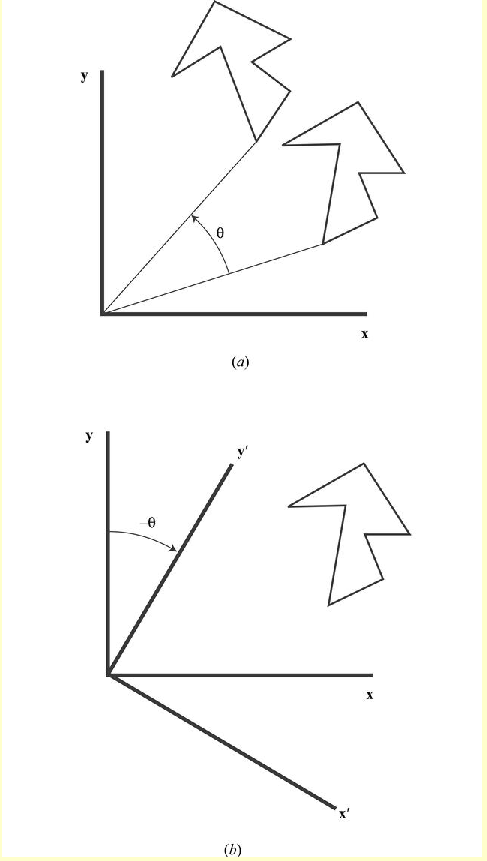
\includegraphics[width=.5\textwidth]{Rotation.png} \end{center}
		In this example the matrix R rotates the vector counter-clockwise given angle $\phi$. An active rotation means that the vector is multiplied by the rotation matrix and this rotates the vector counterclockwise $x' = Rx$. A passive rotation means that the coordinate system is rotated and therefore the vector is also rotated: $x' = R^{-1} x$. Later on we will need rotation matrices for identification of our shocks!
	
	\end{solution}
	
	\item Compute a regular lower triangular matrix $W \in \mathbb{R}^{3 \times 3}$ and a diagonal matrix $\Sigma_\varepsilon \in \mathbb{R}^{3 \times 3}$ such that $\Sigma_u=W \Sigma_\varepsilon W'$.\\Hint: Use the Cholesky factorization $\Sigma_u = P P' = W \Sigma_\varepsilon^{\frac{1}{2}}(W \Sigma_\varepsilon^{\frac{1}{2}})'$.
	\begin{solution}
		\begin{align*}
		\underbrace{\begin{pmatrix}1&0&0\\0&1&0\\0&0.5&1\end{pmatrix}}_W \underbrace{\begin{pmatrix}2.25&0&0\\0&1&0\\0&0&0.49\end{pmatrix}}_{\Sigma_\varepsilon} \underbrace{\begin{pmatrix}1&0&0\\0&1&0.5\\0&0&1\end{pmatrix}}_{W'} = \underbrace{\begin{pmatrix}2.25&0&0\\0&1&0.5\\0&0.5&0.74\end{pmatrix}}_{\Sigma}
		\end{align*}
	\end{solution}
	
	\item Solve the discrete Lyapunov matrix equation $\Sigma_{y} = A\Sigma_{y}A' + \Sigma_{u}$ using
	\begin{enumerate}
		\item the Kronecker product and vectorization
			\begin{solution}
			\begin{align*}
			vec(\Sigma_y) &= vec(A \Sigma_y A') + vec(\Sigma_u) = (A \otimes A)vec(\Sigma_y) + vec(\Sigma_u)\\
			(I-A\otimes A)vec(\Sigma_y) &= vec(\Sigma_u)\\
			vec(\Sigma_y) &= (I-A\otimes A)^{-1}vec(\Sigma_u)
			\end{align*}
			
		\end{solution}
		\item the following iterative algorithm:
			\begin{align*}
			\Sigma_{y,0} &= I, A_0 = A, \Sigma_{u,0} = \Sigma_{u}\\
			\Sigma_{y,i+1} &= A_i \Sigma_{y_i} A_i' + \Sigma_{u,i}\\
			\Sigma_{u,i+1} &= A_i \Sigma_{u,i} A_i' + \Sigma_{u,i}\\
			A_{i+1} &= A_i A_i
			\end{align*}
			Write a loop until either a maximal number of iterations (say 500) is reached or each element of $\Sigma_{y,i+1}-\Sigma_{y,i}$ is less than $10^{-25}$ in absolute terms.
		\begin{solution}

		\end{solution}
	\item Compare both approaches for A and $\Sigma_u$ given above.
	\begin{solution}

		
	\end{solution}
	\end{enumerate}
\begin{solution}
	\lstinputlisting{../progs/MatrixAlgebra.m}
	\lstinputlisting{../progs/dlyapdoubling.m}
\end{solution}

	
\end{enumerate}
\newpage
\section{Understanding multivariate time series concepts}
Let $y_t$ be a K-dimensional time series and $u_t$ a K-dimensional white noise process.
\begin{enumerate}
\item Why are we concerned with multivariate time series? For example, why do we model the VAR(1) process
	\begin{align*}
	\begin{pmatrix}y_{1,t}\\ y_{2,t}\end{pmatrix} = \begin{pmatrix} c_1 \\ c_2\end{pmatrix} + \begin{pmatrix}a_{11} & a_{12}\\ a_{21} & a_{22} \end{pmatrix} \begin{pmatrix}y_{1,{t-1}}\\ y_{2,{t-1}}\end{pmatrix} + \begin{pmatrix}u_{1,t}\\ u_{2,t}\end{pmatrix}
	\end{align*}
	simultaneously instead of two models for each variable separately?
	\begin{solution}
	For the specification of multi-equation models we require a clear distinction between exogenous and endogenous variables. In economic theory this is often not clear or arbitrarily made in practice. Vectorautoregressive models do not need this distinction, they can rather be understood as a dynamic version of a simultaneous multi-equation model. This corresponds to reality, because economic variables are generated by dynamic processes, and often are interdependent. VAR models therefore provide a powerful instrument. They also take into account things like non-stationarity (cointegration and long-term equilibria), as well as the analysis of dynamics of random shocks / impulses. An Example: we are also able to consider correlations between $ u_ {1, t} $ and $ u_ {2, t} $. Lastly, VAR models tend to have better predictive power than multi-equation models and are often used as a benchmark for different forecasting models.
	
	\end{solution}
\item Interpret $E[y_t]$ and $\Gamma_h := Cov[y_{t},y_{t-h}]$.
\begin{solution}
	\emph{Interpretation von $E[y_t]$:} Jede Komponente von $y_t$ hat einen eigenen Erwartungswert. $E[y_t]$ ist somit der unbedingte Erwartungswert von $y_t$ zum Zeitpunkt $t$. Der Erwartungswert als linearer Operator l\"{a}sst sich in einen Vektor oder in eine Matrix hineinziehen:
	\begin{align*}
	E[y_t] = E\left[\begin{pmatrix}y_{1,t} \cr \vdots \cr y_{K,t} \end{pmatrix} \right] = \begin{pmatrix}E[y_{1,t}] \cr \vdots \cr E[y_{K,t}] \end{pmatrix}
	\end{align*}
	\emph{Interpretation of $\Gamma_y(h)$:} In the univariate case we defined the autocovariance as the covariance of a random variable with its own lagged values. In the multivariate case we also consider covariances between different variables. To this end, we want to summarize the covariance between different variables and different points in time. The Autocovariance matrix ${\Gamma_y(h)} := Cov[{y_{t},{y_{t-h}}}]$ sums this information up in a neat fashion and is therefore a powerful tool in multivariate time series analysis:
	\begin{align*}
	&Cov[{y_{t},{y_{t-h}}}] = E\left[({y_{t}}-E[{{y_{t}}}]) ({y_{t-h}}-E[{{y_{t-h}}}])' \right]\\
	&= E\left[\begin{pmatrix}y_{1,t} - E[y_{1,t}] \cr \vdots \cr y_{K,t} - E[y_{K,t}] \end{pmatrix} \begin{pmatrix} y_{1,{t-h}} - E[y_{1,{t-h}}] & \dots & y_{K,{t-h}} - E[y_{K,{t-h}}]  \end{pmatrix} \right]\\
	&= E\left[\begin{pmatrix}
	(y_{1,t}- E[y_{1,t}])(y_{1,{t-h}} - E[y_{1,{t-h}}]) & \dots & (y_{1,t} - E[y_{1,t}])(y_{K,{t-h}} - E[y_{K,{t-h}}])\\
	\vdots & \ddots & \vdots\\
	(y_{K,t}- E[y_{K,t}])(y_{1,{t-h}} - E[y_{1,{t-h}}]) & \dots & (y_{K,t} - E[y_{K,t}])(y_{K,{t-h}} - E[y_{K,{t-h}}])
	\end{pmatrix} \right]\\
	&= \begin{pmatrix}
	E[(y_{1,t}- E[y_{1,t}])(y_{1,{t-h}} - E[y_{1,{t-h}}])] & \dots & E[(y_{1,t} - E[y_{1,t}])(y_{K,{t-h}} - E[y_{K,{t-h}}])]\\
	\vdots & \ddots & \vdots\\
	E[(y_{K,t}- E[y_{K,t}])(y_{1,{t-h}} - E[y_{1,{t-h}}])] & \dots & E[(y_{K,t} - E[y_{K,t}])(y_{K,{t-h}} - E[y_{K,{t-h}}])]
	\end{pmatrix}\\
	&=\begin{pmatrix}
	Cov(y_{1,t},y_{1,{t-h}}) & \dots & Cov(y_{1,t},y_{K,{t-h}})\\
	\vdots & \ddots & \vdots\\
	Cov(y_{K,t},y_{1,{t-h}}) & \dots & Cov(y_{K,t},y_{K,{t-h}})
	\end{pmatrix}
	\end{align*}
	On the diagonals we have the autocovariance of each variable, on the off-diagonals we have the covariances between the different variables.
\end{solution}
\item How does the definition of covariance stationary change in the multivariate case?
\begin{solution}
		Basically it is the same: A stochastic process is called weakly stationary (or covariance stationary), if for each period in time it has the same expectation independent of time and the autocovariance between to points in time is only dependent on the distance of these two points. In the multivariate case we now also consider the autocovariances between different variables and require these to be only dependent on the distance in time, not on time itself.\\
		\texttt{Definition}: The K-dimensional stochastic process $y_t$ is called covariance stationary, if for all $h,t,\tau \in \mathbb{Z}$:
		\begin{align}
		E[{y_t}] &= E[{y_\tau}]\\
		Cov(y_{t},y_{t-h}) &= Cov(y_{t+\tau}, y_{t-h+\tau}) \label{gammas}
		\end{align}
\end{solution}
\item Consider the following VAR(1) process $y_t = c + A y_{t-1} + u_t$
\begin{align*}
\begin{pmatrix}y_{1,t} \\ y_{2,t}\\y_{3,t} \end{pmatrix} &= \begin{pmatrix}0\\0\\0 \end{pmatrix} + \begin{pmatrix}0.5 &0 &0 \\0.1&0.1&0.3\\0&0.2&0.3 \end{pmatrix} \begin{pmatrix}y_{1,{t-1}} \\ y_{2,{t-1}}\\y_{3,{t-1}} \end{pmatrix} + \begin{pmatrix}u_{1,t} \\ u_{2,t}\\ u_{3,t} \end{pmatrix}
\end{align*}
provided that $u_t \sim WN(0,\Sigma_u)$ and $$\Sigma_u = \begin{pmatrix}2.25 & 0 & 0\\ 0 & 1 & 0.5\\ 0 & 0.5 & 0.74 \end{pmatrix}$$
Compute the coefficients $\Phi_0, \Phi_1, \dots \in \mathbb{R}^{3\times 3}$ of the lag polynomial $\Phi(L) := \sum_{i=0}^\infty \Phi_i L^i$, and a $\nu \in \mathbb{R}^3$ such that
\begin{align*}
y_t = \nu + \Phi(L) u_t
\end{align*}
\begin{solution}
		We will use the very efficient method of matching coefficients to transform the VAR(1) model into a VMA($\infty$) representation.
		\begin{align*}
		y_t &= A y_{t-1} + u_t\\
		\underbrace{(I_3 - A L)}_{A(L)} y_t &= u_t\\
		A(L) y_t &= u_t \\
		A(L)^{-1}A(L) y_t &= A(L)^{-1} u_t\\
		y_t &= A(L)^{-1} u_t = \nu + \Phi(L) u_t\\
		\Rightarrow & \nu= 0, \Phi(L) = A(L)^{-1}
		\end{align*}
		In the method of matching coefficient we compare the coefficient matrices multiplied to each power of $L$. That is, the expression on the left hand side has to match the expression on the right hand side. In our case:
		\begin{align*}
		\Phi(L) &= A(L)^{-1}\\
		A(L) \Phi(L) &= I_3\\
		(I_3 - A L) \left(\sum_{i=0}^\infty \Phi_i L^i\right) &= I_3
		\end{align*}
		\begin{align*}
		\Phi_0 L^0 &+ \Phi_1 L^1 + \Phi_2 L^2 + \dots \\
		& - A \phi_0 L^1 - A \phi_1 L^2 - \dots = I_3 L^0
		\end{align*}
		\begin{align}
		L^0&: \Phi_0 &= I_3 \Rightarrow& \Phi_0 = I_3 = \begin{pmatrix}1&0&0\\0&1&0\\0&0&1 \end{pmatrix}\nonumber\\
		L^1&: \Phi_1 - A \Phi_0 &= 0 \Rightarrow& \Phi_1 = A \Phi_0 = A = \begin{pmatrix}0.5&0&0\\0.1&0.1&0.3\\0&0.2&0.3 \end{pmatrix}\nonumber\\
		L^2&: \Phi_2 - A \Phi_1 &= 0 \Rightarrow& \Phi_2 = A \Phi_1 = A^2 = \begin{pmatrix}0.25&0&0\\0.06&0.07&0.12\\0.02&0.08&0.15 \end{pmatrix}\nonumber\\
		\vdots\nonumber\\
		&\text{In general}: \Phi_s = A^s \label{allg}
		\end{align}
\end{solution}
\end{enumerate}


\newpage
\section{Dimensions and VAR(1) representation}
Let $y_t$ be a K-dimensional covariance stationary random vector. Consider the VAR(p)-process
\begin{align*}
y_t = c + \sum_{i=1}^p A_i {y_{t-i}} + u_t
\end{align*}
\begin{enumerate}
\item What are the dimensions of $\nu, A_i$ and $u_{t}$?
\begin{solution}
	$\nu$ snd $u_t$ are both K-dimensional vectors: $\nu,u_t \in \mathbb{R}^{K \times 1}$. $A_i$ is a $K \times K-$Matrix.
\end{solution}
\item Assume that $E(u_t) = 0; E(u_t u_t') = \Sigma_u$ with $\Sigma_u$ being symmetric and positive definite. Which additional assumptions do we need to assure that $u_t$ is a multivariate white noise process?
\begin{solution}
	
		We must have ${\Gamma_u(h)} = Cov(u_t, u_{t-h}) = 0_{K\times K},s\neq0$, that is all autocovariances are zero for $h\neq0$. We do not need a distributional assumption!
\end{solution}
\item Consider a VAR(2) model with K=4 variables and a constant term. How many parameters do we need to estimate?
\begin{solution}
	
		General: $K$ constants + $K^2\cdot p$ Autoregressive coefficients + $K(K+1)/2$ covariance terms. Here: $4+4^2\cdot2+4\cdot(4+1)/2=46$. That's a lot! Therefore we will try to restrict some parameters (e.g. set equal to zero) or consider only small VAR systems, e.g. K=3 p=1.
	
\end{solution}
\item Show how to represent a VAR(3) model as a VAR(1) model. Write a function that transforms any VAR(p) model into VAR(1), i.e. its \enquote{companion form}.
\begin{solution}
	VAR(3): $y_t = \nu + A_1 y_{t-1} + A_2 y_{t-2} + A_3 y_{t-3} + u_t$. Idea: Stack $y_t, y_{t-1}$ and $y_{t-2}$ into a vector and note that $y_{t-1}=y_{t-1},y_{t-2}=y_{t-2}$. That is
\begin{align*}
\underbrace{\begin{bmatrix} y_t\\ y_{t-1} \\ y_{t-2} \end{bmatrix}}_{\widetilde{y}_t} = \underbrace{\begin{bmatrix} A_1 & A_2 & A_3 \\ I & 0 & 0\\ 0&I&0\end{bmatrix}}_{\widetilde{A}} \underbrace{\begin{bmatrix} y_{t-1}\\ y_{t-2} \\ y_{t-3} \end{bmatrix}}_{\widetilde{y}_{t-1}} + \underbrace{\begin{bmatrix} u_t \\ 0 \\ 0\end{bmatrix}}_{\widetilde{u}_t}
\end{align*}
Therefore: $\widetilde{y}_t = \widetilde{A} \widetilde{y}_{t-1} + \widetilde{u}_t$. This is called the Companion Form.

	\lstinputlisting{../progs/CompanionForm.m}
\end{solution}
\end{enumerate}
\newpage


\section{Theoretical and simulated moments}
\begin{enumerate}
	\item Derive the theoretical mean, covariance and autocovariance matrix of the covariance stationary VAR(1) model: $y_t = c + A y_{t-1} + u_t$
	\begin{solution}
	\begin{align*}
		\underbrace{E(y_t)}_{\mu_y} &= \underbrace{E(\nu)}_{\nu} + \underbrace{E(A y_{t-1})}_{A \mu_y} + \underbrace{E(u_t)}_{0}\\
		\Leftrightarrow \mu_y &= (I-A)^{-1} \nu
		\end{align*}
		Put $v = (I-A)\mu_y: \underbrace{y_t -\mu_y}_{\tilde{y}_{t}} = A(\underbrace{y_{t-1}-\mu_y}_{\tilde{y}_{t-1}}) + u_t$. note: $\Gamma_y(h) = \Gamma_{\tilde{y}(h)}$
		\begin{align*}
		\Gamma_y(0) &= E\left[\tilde{y}_t \tilde{y}_t'\right]= E\left[(A \tilde{y}_{t-1} + u_t)(A \tilde{y}_{t-1} + u_t)'\right]\\
		&= A \underbrace{E\left[\tilde{y}_{t-1}\right]}_{\Gamma_y(0)} A' + A \underbrace{E\left[\tilde{y}_{t-1}u_t'\right]}_{0} + \underbrace{E\left[u_t \tilde{y}_{t-1}'\right]}_{0} A' + \underbrace{E\left[u_t u_t'\right]}_{\Sigma_u}\\
		\Leftrightarrow \Gamma_y(0) &= A \Gamma_y(0) A' + \Sigma_u
		\end{align*}
		This is a discrete Lyapunov matrix equation, see exercise 1.5: $$vec(\Gamma_y(0)) = (I-A \otimes A)^{-1} vec(\Sigma_u)$$
		\begin{align*}
		\Gamma_y(1) &=  E\left[\tilde{y}_t \tilde{y}_{t-1}'\right]= E\left[(A \tilde{y}_{t-1} + u_t)\tilde{y}_{t-1}'\right] = A E\underbrace{\left[\tilde{y}_{t-1}\tilde{y}_{t-1}'\right]}_{\Gamma_y(0)} + \underbrace{E\left[u_t y_{t-1}'\right]}_{0} = A \Gamma_y(0)\\
		\Gamma_y(2) &=  E\left[\tilde{y}_t \tilde{y}_{t-2}'\right]= E\left[(A \tilde{y}_{t-1} + u_t)\tilde{y}_{t-2}'\right] = A \Gamma_y(1) = A^2 \Gamma_y(0)\\
		\Gamma_y(h) &= A^h \Gamma_y(0)
		\end{align*}
	\end{solution}
	\item Simulate $R=100$ datasets each with $T=100$ observations for
	\begin{align*}
	y_t = \begin{pmatrix}0.2 &0.3 \\-0.6 & 1.1 \end{pmatrix} y_{t-1}  + u_t
	\end{align*}
	provided that $u_t \sim WN(0,\Sigma_u)$ and $\Sigma_u = \begin{pmatrix}0.9 &  \\ 0.2 & 0.5 \end{pmatrix}$. \\Compute the sample mean and sample covariance matrix. Compare the results with parts (1) and (2). How does your choice of R or T change results?
	\begin{solution}
	\lstinputlisting{../progs/VarMomentsMonteCarlo.m}
	The Monte Carlo shows that either increasing R or T (or both) captures the moments better.
	\end{solution}
\end{enumerate}
\newpage

\section{Ordinary Least Squares Estimation of VAR(p)}
Consider the VAR(p) model with constant written in the more compact form
$$ y_t = [c, A_1, ..., A_p] Z_{t-1} + u_t = A Z_{t-1}+ u_t$$
where $Z_{t-1}=(1,y_{t-1}',...,y_{t-p}')'$ and $u_t$ is assumed to be iid white noise with nonsingular covariance matrix $\Sigma_u$. Given a sample of size $T$, $y_1,...,y_T$, and $p$ presample vectors, $y_{-p+1},...,y_{0}$, ordinary least squares for each equation separately results in efficient estimators. The OLS estimator is
$$\hat{A} = \left[ \hat{c}, \hat{A_1},...,\hat{A_p}\right] = \left(\sum_{t=1}^{T}y_t Z_{t-1}'\right)\left(\sum_{t=1}^{T}Z_{t-1}Z_{t-1}'\right)^{-1} = Y Z'(ZZ')^{-1}$$
where $Y=[y_1,...,y_T]$ and $Z=[Z_0,...,Z_{T-1}]$. More precisely, stacking the columns of $A = [c, A_1,...,A_p]$ in the vector $\alpha = vec(A)$,
$$\sqrt{T}\left(\hat{\alpha} - \alpha \right) \overset{d}{\rightarrow} \mathcal{N}(0, \Sigma_{\hat{\alpha}})$$
where $\Sigma_{\hat{\alpha}} = plim(\frac{1}{T}ZZ')^{-1}\otimes \Sigma_u$, if the process is stable. Under fairly general assumptions this estimator has an asymptotic normal distribution. A sufficient condition for the consistency and asymptotic normality of $\hat{A}$ would be that $u_t$ is a continuous iid random variable with four finite moments. A consistent estimator of the innovation covariance matrix $\Sigma_u$ is, for example,
$$\hat{\Sigma}_u = \frac{\hat{U}\hat{U}'}{T-Kp-1}$$
where $\hat{U} = Y - \hat{A}Z$ are the OLS residuals. Thus, in large samples,
$$vec(\hat{A}) \overset{a}{\sim}\mathcal{N}(vec(A),(ZZ')^{-1}\otimes \hat{\Sigma}_u)$$
where $\overset{a}{\sim}$  denotes the approximate large-sample distribution. In other words,
asymptotically the usual t-statistics can be used for testing restrictions on individual coefficients and for setting up confidence intervals.
\begin{enumerate}
	\item What are the dimensions of $y_t$, $Y$, $u_t$, $U$, $c$, $A_1$, ..., $A_p$, $A$, $\alpha$, $Z_{t-1}$, $Z$, $\Sigma_u$ and $\Sigma_{\hat{\alpha}}$.
	\begin{solution}		
		$y_t$ is $K \times 1$, $Y$ is $K \times T$, $u_t$ is $K \times 1$, $U$ is $K \times T$, $c$ is $K \times 1$, $A_1$ is $K \times K$, ..., $A_p$ is $K \times K$, $A$ is $K \times (1+pK)$, $\alpha$ is $(pK^2+K) \times 1$, $Z_{t-1}$ is $(1+pK) \times T$, $Z$ is $(Kp+1) \times T$, $\Sigma_u$ is $K \times K$ and $\Sigma_{\hat{\alpha}}$ is $(pK^2+K) \times (pK^2+K)$.
	\end{solution}
	\item Consider data for $y_t = (\Delta gnp_t,i_t,\Delta p_t)'$, where $gnp_t$ denotes the log of U.S. real GNP, $p_t$ the corresponding GNP deflator in logs, and $i_t$ the federal funds rate, averaged by quarter. The estimation period is restricted to 1954q4-2007q4. Load the data from  \texttt{data.xlsx} and visualize it. Comment whether you think the data looks stationary.
	\begin{solution}
		The data for Federal Funds Rate as well as the GNP Deflator Inflation does seem to have some trend in it.
	\end{solution}
	\item Estimate a VAR(4) model using the \texttt{VARReducedForm.m} function. This is basically a modified version of your \texttt{ARpOLS.m} function. Examine the stability of the estimated process and the significance of the estimated parameters using t-ratios at a $95\%$ level.
	\begin{solution}
		\lstinputlisting{../progs/ThreeVariableVAR.m}
	\end{solution}
\end{enumerate}

\section{Maximum Likelihood Estimation of VAR(p)}
Consider the VAR(p) model with constant written in the more compact form
$$ y_t = [c, A_1, ..., A_p] Z_{t-1} + u_t = A Z_{t-1}+ u_t$$
where $Z_{t-1}=(1,y_{t-1}',...,y_{t-p}')'$. In VAR analysis, it is common to postulate that the innovations, $u_t$, are iid $\mathcal{N}(0,\Sigma_u)$ random variables. This assumption implies that the $y_t$'s are also jointly normal and, for given initial values $y_{-p+1},...,y_{0}$,
$$f_t(y_t|y_{t-1},...,y_{-p+1})=\left(\frac{1}{2\pi}\right)^{K/2} det(\Sigma_u)^{-1/2}exp\left\{-\frac{1}{2}u_t'\Sigma_u^{-1}u_t\right\}$$ 
Hence, the log-likelihood becomes (see also exercise \ref{ex:MLARp}):

$$\log l = -\frac{KT}{2}\log(2\pi) - \frac{T}{2}log(det(\Sigma_u))- \frac{1}{2}\sum_{t=1}^Tu_t'\Sigma_u^{-1}u_t$$
Maximizing this function with respect to the unknown parameters yields the Gaussian ML estimator.
\begin{enumerate}
	\item Compare the Gaussian ML estimator with the OLS estimator from the previous exercise. Comment on the asymptotic distribution.
	\begin{solution}
		They are identical, hence the asymptotic normality holds as well.
	\end{solution}
	\item Provide an expression for the ML estimator of the innovation covariance matrix.
	\begin{solution}
		$$\tilde{\Sigma}_u(m) = \frac{T-Km-1}{T}\hat{\Sigma}_u(m)$$
	\end{solution}
	\item Redo the estimation from the previous exercise.
	\begin{solution}
		\lstinputlisting{../progs/ThreeVariableVAR.m}
	\end{solution}
\end{enumerate}

\newpage
\section{Information Criteria for VAR(p)}
Information criteria used for VAR lag order selection have the general form (see also exercise \ref{ex:InfoARp}):
$$C(m) = log(det(\tilde{\Sigma_u})) + c_T \varphi(m)$$
where $\tilde{\Sigma}_u=T^{-1}\sum_{t=1}^T \hat{u}_t\hat{u}_t'$ is the residual covariance matrix estimator for a reduced-form VAR model of order $m$ based on OLS residuals $\hat{u}_t$, $\varphi(m)$ is a function of the order $m$ that penalizes large VAR orders and $c_T$ is a sequence of weights that may depend on the sample size.
The function $\varphi(m)$ corresponds to the total number of regressors in the system of VAR equations. Since there are one intercept and $mK$ lagged regressors in each equation and K equations in the VAR model, $\varphi(m)= mK^2 + K$. Information criteria are based on the premise that there is a trade-off between the improved fit of the VAR model, as $m$ increases, and the parsimony of the model. Given $T$, the fit of the model by construction improves with larger $m$, indicated by a reduction in $\log(det(\tilde{\Sigma}_u(m)))$. At the same time the penalty term, $c_T \varphi(m)$, unambiguously increases with $m$. We are searching for the value of $m$ that balances the objectives of model fit and parsimony. The choice of the penalty term determines the trade-off between these conflicting objectives. 

The three most commonly used information criteria for VAR models are known as the Akaike Information Criterion (AIC), Schwarz Information Criterion (SIC) and Hannan-Quinn Criterion (HQC):
\begin{align*}
AIC(p)  &= \log(det(\tilde{\Sigma}_u(m))) + \frac{2}{T}\varphi(m)\\
SIC(p)  &= \log(det(\tilde{\Sigma}_u(m))) + \frac{\log T}{T}\varphi(m)\\
HQC(p)  &= \log(det(\tilde{\Sigma}_u(m))) + \frac{2\log (\log T)}{T}\varphi(m)
\end{align*}

The VAR order is chosen such that the respective criterion is minimized over the possible orders $m = p^{min},...,p^{max}$. A key issue in implementing information criteria is the choice of the upper and lower bounds. In the context of a model of unknown finite lag order, the default is to set $p^{min}=0$ or sometimes $p^{min} = 1$. The value of $p^{max}$ must be chosen long enough to allow for delays in the response of the model variables to the shocks. In practice, common choices would be 12 or 24 lags for monthly data and 4 or 8 lags for quarterly data.
\begin{enumerate}
	\item Why is it essential that for a given lag order we compute $\tilde{\Sigma}_u(m)$ on exactly the same evaluation period, $t=p^{max}+1,...T$, for all $m$?
	\begin{solution}
		If the evaluation period used in computing $\tilde{\Sigma}_u(m)$ differs across $m \in \{1,...,p^{max}\}$, we risk that differences in the fit of different models are driven by the inclusion of additional observations rather than the inclusion of additional lags. In other words, we end up comparing apples and oranges, rendering the resulting ranking meaningless. For example, many canned software packages produce AIC values as a by-product of the regression output. It may seem that these values could be used to rank alternative VAR models according to their AIC values. This is not the case. The reason is that the relevant evaluation period for computing $\tilde{\Sigma}_u(m)$ depends on $p^{max}$. Without the user specifying $p^{max}$, canned software packages cannot possibly compute the correct estimate $\tilde{\Sigma}_u(m)$ or the corresponding AIC values. Instead, they may display AIC values based on the evaluation period $t = m + 1,..., T$, where $p^{min} \leq m \leq p^{max}$. It may seem that this mistake could not have important consequences, but Ng and Perron (2005) demonstrate by simulation that this mistake can result in severe distortions in the estimated order $\hat{p}$.
	\end{solution}
	\item Why is it essential, that the criterion function be evaluated at the ML estimator $\tilde{\Sigma}_u=T^{-1}\sum_{t=1}^T \hat{u}_t\hat{u}_t'$ rather than the OLS estimator $\hat{\Sigma}_u=(T-Km-1)^{-1}\sum_{t=1}^T \hat{u}_t\hat{u}_t'$?
	\begin{solution}
	The use of information criteria is predicated on the trade-off between improved fit (measured by decline in $det(\tilde{\Sigma}_u(m))$ and the reduction in parsimony (measured by an increase in the penalty term), as more lags are added. There is no such trade-off when we estimate $\Sigma_u(m)$ by 
	$$\hat{\Sigma}_u(m) = \frac{T}{T-Km-1}\tilde{\Sigma}_u(m)$$
	Adding more lags lowers	$det(\tilde{\Sigma}_u(m))$ by construction, but also increases $\frac{T}{T-Km-1}$, invalidating the model rankings.
	\end{solution}
	\item Comment on the asymptotically and finite-sample properties of the criteria.
	\begin{solution}
%%		If the DGP is a VAR(p 0 ) model, one criterion is whether the lag order estimator
%%		is consistent for the true lag order p 0 , provided p min ≤ p 0 ≤ p max . Clearly,
%%		sequential tests will not be consistent for p 0 because of the positive probability
%%		of committing a type I error in statistical testing. In contrast, information
%%		criteria will be consistent for p 0 under suitable conditions. The reason is that
%%		the probability of committing a type I error vanishes asymptotically, if we are
%%		careful about the choice of penalty function. As is easy to verify, the AIC
%%		is not consistent for p 0 , whereas the SIC and HQC are (see Lütkepohl (2005,
%%		Section 4.3.2)). The HQC was designed to be the least parsimonious, yet still
%%		consistent information criterion for VAR models. Although standard proofs of
%%		the consistency of the SIC and HQC and of the inconsistency of the AIC require
%%		the VAR model to be stationary, these results can be extended to VAR models
%%		with unit roots (see Paulsen (1984), Tsay (1984)).
%%		The price of obtaining a consistent lag order estimator is greater parsimony
%%		in model selection. Parsimony here means that the criterion will favor VAR
%%		models with fewer lags. The larger the penalty term for given T , the more
%%		parsimonious the lag order estimate. It can be shown that for T ≥ 16,
%%		indicating that the SIC tends to be more parsimonious than the HQC, which
%%		in turn tends to be more parsimonious than the AIC. Of course, in a given
%%		application, all three criteria may suggest the same lag order.
%%		Finite-Sample Properties of the Lag Order Estimator
%%		Even if we grant the premise that p min ≤ p 0 ≤ p max , one may not want to
%%		overrate the importance of the lag order estimator being consistent. The con-
%%		consistent lag order selection criteria tend to be strongly downbiased toward
%%		p min . For example, Kilian (2001) examines a stylized bivariate AR(4) data gen-
%%		erating process and shows that for a sample size of T = 80, the SIC selects a ag order of 1 among 1 ≤ p ≤ 8 with probability 92%, but the true lag order
%%		of 4 only with probability 2%. Even for T = 160, the probability of selecting
%%		p = 1 remains at 61% with a probability of only 28% of selecting the true lag
%%		order. Similar, if less extreme results hold for the HQC. In contrast, the AIC
%%		has a probability of selecting the true lag order of 57% for T = 80 and of 83%
%%		for T = 160. The probability of the AIC underestimating the lag order is 26%
%%		for T = 80 and 1% for T = 160, compared with 98% and 73% for the SIC. The
%%		finding that in small samples the distribution of the AIC lag order estimates
%%		tends to be more balanced about the true lag order than for the SIC lag order
%%		estimates is also consistent with simulation results in Nickelsburg (1985) and
%%		Lütkepohl (1985).
%%		The high accuracy of the AIC in these simulation studies - even in large
%%		samples - may be surprising at first, but reflects the asymptotic properties of
%%		the AIC. Although
%%		reflecting the inconsistency of the AIC, it can be shown that
%%		In other words, in the limit, the AIC will never select a lag order that is lower
%%		than p 0 , but it will have a tendency to select with positive probability a lag
%%		order in excess of p 0 . This point is important. Economists using VAR models
%%		have no inherent interest in the lag order of the process. They are interested
%%		in impulse responses, forecasts, and related statistics that can be written as
%%		smooth functions of VAR model parameters. These statistics of interest can be
%%		consistently estimated, as long as the lag order is not underestimated asymp-
%%		totically, so there is little to choose between the SIC, HQC, and AIC on the
%%		grounds of consistency. The only potential concern is that in large samples the
%%		AIC may choose an excessively large lag order and inflate, for example, the
%%		variance of the impulse response estimator.
%%		This concern as well is largely unfounded. Paulsen and Tjøstheim (1985)
%%		establish that the probability of the AIC overfitting the VAR model is negligible
%%		asymptotically. Whereas for K = 1, the asymptotic probability of overfitting
%%		is about 30%, for K = 2 it drops to at most 12%, for K = 3 to 4%, and for
%%		K = 4 to 1%, so for most VAR applications, the efficiency loss is not a major
%%		concern. These asymptotic results are consistent with simulation evidence for
%%		large-dimensional VAR models in Gonzalo and Pitarakis (2002) who conclude
%%		that the AIC tends to be by far the most reliable estimator of p 0 compared with
%%		sequential tests as well as other information criteria.
%%		Finite-sample considerations also favor the AIC. In related work, Kilian
%%		(2001) observes that in the context of impulse response analysis in finite sam-
%%		ples overestimation of the lag order is costly only to the extent that the impulse
%%		response estimates are less precise, but underestimation tends to greatly distort
%%		the impulse response functions especially at longer horizons. Hence, users ofVAR models ought to employ an asymmetric loss function, erring on the side of
%%		including too many lags. Kilian (2001) provides simulation evidence that VAR
%%		models based on the AIC lag order estimate provide more accurate impulse re-
%%		sponse confidence intervals than VAR models based on more parsimonious lag
%%		order selection criteria. He also shows that AIC-based impulse response esti-
%%		mates have lower MSE. This conclusion is further supported by simulation evi-
%%		dence in Kilian and Ivanov (2005) based on a wide range of monthly finite-order
%%		VAR models of the type used in empirical work. Kilian and Ivanov show that for
%%		monthly VAR models the AIC implies impulse response estimates with system-
%%		atically lower MSE than more parsimonious criteria such as the SIC or HQC.
%%		For quarterly VAR models, which tend to imply smoother impulse responses,
%%		using the HQC generates the impulse response estimates with the lowest MSE.
%%		There also is simulation evidence on the performance of sequential tests for
%%		lag order selection. At least for univariate autoregressions, several studies have
%%		shown that the general-to-specific sequential-testing approach is preferred to
%%		the specific-to-general sequential testing approach. For VAR models neither ap-
%%		proach is satisfactory for selecting the true lag order (see, e.g., Lütkepohl (1985);
%%		Nickelsburg (1985); Gonzalo and Pitarakis (2002)). Moreover, the simulation
%%		evidence in Kilian and Ivanov (2005) shows that sequential testing procedures
%%		tend to produce impulse response estimators with systematically larger MSE
%%		than information criteria and cannot be recommended for applied work.
	\end{solution}
	\item Let $m=\{0,1,...,4\}$. Select the lag-order according to the information criteria for the three-variable VAR model used in the previous two exercises.
	\begin{solution}
	%ble 2.1 illustrates the implementation of the SIC, HQC, and AIC criteria in
	%the context of the three-variable VAR model example already used earlier in this
	%chapter to illustrate alternative estimation procedures. Let m ∈ {0, 1, . . . , 4}.
	%The lag order values that minimize a given criterion function are shown in bold.
	%Table 2.1 shows that the SIC favors a lag order of p = 1, whereas the HQC
	%chooses a lag order of p = 3, and the AIC chooses p = 4.
	\end{solution}
\end{enumerate}

\section{Bayesian Estimation Basics}
\begin{enumerate}
	\item Consider a simple model:
	$$y_t = \mu + u_t$$
	with $t = 1, 2,..., T$ and $u_t \sim \mathcal{N}(0,\sigma^2)$. Assume that $\sigma^2$ is known, thus, we want to estimate $\mu$. How do classical and Bayesian analysis differ?
	\item Name the key ingredients for Bayesian analysis.
	\item What are \enquote{conjugate priors} and \enquote{natural conjugate priors}?
	
\end{enumerate}
\newpage
\section{Bayesian Estimation Of Multivariate Linear Regression Model}
Consider a linear regression model with multiple regressors:
$$Y = X\beta + u$$ with $u \sim \mathcal{N}(0, \sigma^2 I)$.
\begin{enumerate}
	\item Name the idea and general procedure when estimating this model with Bayesian methods.
	\item Provide an expression for the likelihood function $p(Y|\beta,\sigma^2)$.
	\item Assume that $\sigma^2$ is known and the prior distribution for $\beta$ is Gaussian with mean $\beta_0$ and covariance matrix $\Sigma_0$. Derive an expression for the posterior distribution $p(\beta|\sigma^2,Y)$.
	\item Assume that $\beta$ is known and the prior distribution for $1/\sigma^2$ is Gamma with shape parameter $s_0$ and scale $v_0$. Derive an expression for the posterior distribution $p(1/\sigma^2|\beta,Y)$.
	\item Now assume that both $\beta$ and $\sigma^2$ are unknown. Provide intuition behind and an overview of the basic steps of the Gibbs sampling algorithm.
\end{enumerate}
\newpage
\section{Bayesian Estimation Of Quarterly Inflation}
Perform a Bayesian estimation of an AR(2) model of quarterly inflation with the Gibbs sampler by assuming a Gamma distribution for the marginal prior for $\sigma^2$ and a normal distribution for the conditional prior for $\beta$ given $1/\sigma^2$. To this end, do the following:
\begin{enumerate}
	\item Load the dataset given in data.xlsx for quarterly inflation from 1947Q1 to 2012Q3
	\item Generate the matrix of regressors for the AR(2) model with constant, call it X, and a vector of endogenous variables, call it y.
	\item Set the prior mean for the coefficients to a vector of zeros and the prior covariance matrix to the identity matrix. Set the shape parameter for the variance parameter to 1 and the scale parameter to 0.1. Initialize the first draw of $1/\sigma^2$ to 1.
	\item Set the total number of Gibbs iterations to 5000 with a burn-in phase of 4000. Initialize output matrices for the remaining 1000 draws for the coefficient estimates and the variance estimate.
	\item For $j=1,...,5000$ do the following	
	\begin{enumerate}	
		\item Sample $\beta(j)$ conditional on $1/\sigma^2(j)$ from $\mathcal{N}(M,V)$ where 
		$$M=(\Sigma_0^{-1}+\sigma^2(j) (X'X))^{-1} \cdot (\Sigma_0^{-1}\beta_0+\sigma^2(j) X'y)$$ and 
		$$V=(\Sigma_0^{-1} +\sigma^2(j)(X'X))^{-1}$$
		Optional: check the stability of the draw to avoid an explosive AR processes.
		\item Sample $1/\sigma^2(j)$ conditional on $\beta(j)$ from the inverse Gamma distribution $IG(s_1,v_1)$ where $s_1 = s_0 + T$ and $v_1 = v_0 + (y-X\beta(j))'(y-X\beta(j))$. A draw from the inverse gamma distribution can be generated from $v_1/(z' z)$ where $z$ are $s_1$ draws from a standard normal distribution.
		\item If you passed the burn-in phase, then save the draws of $\beta(j)$ and $1/\sigma^2(j)$.
	\end{enumerate}
	\item Plot the marginal posterior distributions, i.e. look at the histograms.
	\item Compare the mean of your posterior draws with the OLS estimates.
\end{enumerate}

\newpage
\section{Bayesian Estimation Of VAR(p)}
Consider the following K-variable VAR(p) model:
$$y_t = c + A_1 y_{t-1} + ... + A_p y_{t-p} + u_t= AZ_{t-1} + u_t$$ where $E(u_t)=0$, $E(u_t u_t')=\Sigma_{u}$ and $E(u_t u_s')=0$ for $t\neq s$. Define $\alpha = vec(A)$ and assume that $\varepsilon_t|y_{t-1},...,y_1\sim N(0,\Sigma)$.
\begin{enumerate}
	\item Explain why Bayesian methods are especially attractive when estimating a VAR(p) model.
	\item Assume that the prior for $\alpha$ is normal with mean $\alpha_0$ and covariance matrix $V_0$. Provide an expression for the posterior conditional on $\Sigma$.
	\item Assume that the prior for the VAR covariance matrix $\Sigma$ is inverse Wishart with degrees of freedom $v_0$ and scale matrix $S_0$. Provide an expression for the posterior conditional on $\alpha$. 
	\item Briefly outline the basic steps of the Gibbs sampling algorithm given the conditional posteriors.
	\item Provide intuition behind the \enquote{Minnesota prior}.\\\emph{Hint: Have a look at the \texttt{BVARPrior.m} function.}
	\item Provide intuition behind the \enquote{independent normal-inverse Wishart prior}.\\\emph{Hint: Have a look at the \texttt{BVARPrior.m} function.}
\end{enumerate}

\newpage

\section{Bayesian Estimation Of VAR(2) At Zero-Lower-Bound}
Consider a VAR(p) model for the US economy which includes (in this ordering) the federal funds rate, government bond yield, unemployment and inflation. The sample period consists of 2007m1 to 2010m12. Data is given in the excel sheet \enquote{USZLB} in the file \texttt{data.xlsx}.\\
\begin{enumerate}
	\item Estimate the parameters of a VAR(2) model with constant by using Bayesian methods, i.e. a Gibbs sampling method where you assume a Minnesota prior for the VAR coefficients and a inverse wishart prior for the covariance matrix.\\To this end:
	\begin{itemize}
	\item Define a Minnesota prior for the VAR coefficients. The prior mean $a_0$ should reflect the view that the VAR follows a random walk. Set the hyperparameters for the prior covariance matrix $V_0$ such that the tightness parameter on lags of own variables is equal to 0.5, the one on lags of other variables is also equal to 0.5 and the tightness parameter on the constant term is equal to 1.
	\item Define an Inverse Wishart prior for the covariance matrix with degrees of freedoms $v_0$ equal to the number of variables and the identity matrix as prior scale matrix $S_0$. 
	\item Initialize the first draw of the covariance matrix with OLS values.
	\item Draw 40000 times from the conditional posteriors $$p(vec(A)|\Sigma,Y) \sim N(a_1,V_1)$$ and $$p(\Sigma|vec(A),Y) \sim IW(v_1, S_1)$$ where
	\begin{align*}
	V_1 &= (V_0^{-1}+ZZ' \otimes \Sigma^{-1})^{-1}\\
	a_1 &= V_1 (V_0^{-1}a_0 + (Z \otimes \Sigma^{-1})vec(Y))\\
	v_1 &= T + v_0\\
	S_1 &= S_0 + (Y - A*Z)(Y - A*Z)'
	\end{align*}
	and keep the last 10000 draws for inference. 
	\item Check the stability of the draws of the coefficient matrix $A$, i.e. compute the eigenvalues of the companion matrix and discard the draw if the modulus of all eigenvalues of the companion form is larger than one.
	\end{itemize}
	\item As the sample period includes the financial crisis, redo the exercise but now use a small prior variance to reflect the view that monetary policy is at the zero-lower-bound and hence unlikely to respond to changes in the other variables.	
\end{enumerate} 
\newpage

\section{Identification Problem in Structural Vector Autoregressions}
Consider a simple 2-variable model:
\begin{align*}
i_t &=  \beta \pi_t + \gamma_1 i_{t-1} + \gamma_2 \pi_{t-1} + \sigma_{MP} \varepsilon_t^{MP} \\
\pi_t &=  \delta i_t + \gamma_3 i_{t-1} + \gamma_4 \pi_{t-1} + \sigma_{\pi} \varepsilon_t^{\pi}
\end{align*}
where $i_t$ denotes the interest rate set by the central bank and $\pi_t$ the inflation rate. Assume 
for the structural shocks: $\varepsilon_{t}=(\varepsilon_t^{MP}, \varepsilon_t^{\pi})' \sim N(0,I_2)$.
\begin{enumerate}
	\item Rewrite the model in a compact matrix form $B_0 y_t = B_1 y_{t-1} + \varepsilon_{t}$. Note that this is a structural VAR(1) model.
	\item Since the structural VAR model is not directly observable, derive the reduced-form representation: $y_t=A_1 y_{t-1} + u_t$. What is the relationship between structural shocks $\varepsilon_t$ and reduced-form residuals $u_t$?
	\item Consider the dynamic causal effect of the monetary policy shock $\varepsilon_t^{MP}$ on $y_t$, i.e. an interest rate increase while holding all other interventions constant: In other words, derive the impulse response function (IRF) of $y_t$ to the shock $\varepsilon_t^{MP}$: $$\frac{\partial y_{t+h}}{\partial \varepsilon_t^{MP}}, \text{ for } h=1,2,3,...$$
	\item In your own words, explain the identification problem in SVAR models. Provide intuition behind the popular identification assumptions of short-run, long-run and sign restrictions.
\end{enumerate}
\newpage

\section{Structural Impulse Responses}
Consider the structural VAR(p) model $$y_t = B_1 y_{t-1} + ... + B_{p} y_{t-p} + \varepsilon_{t}$$
where the dimension of $B_i$, $i = 0,...,p$, is $K \times K$. The $K \times 1$ vector of structural shocks $\varepsilon_{t}$ is assumed to be white noise with covariance matrix $E(\varepsilon_t \varepsilon_t') = I_K$. That is, the Elements of $\varepsilon_t$ are mutually uncorrelated and also have a clear interpretation in terms on an underlying economic model. The reduced-form VAR(p) model is given by
$$y_t = \underbrace{B_0^{-1}B_1}_{A_1}y_t + ... + \underbrace{B_0^{-1}B_p}_{A_p} y_{t-p} + \underbrace{B_0^{-1}\varepsilon_t}_{u_t}$$
where the reduced-form error covariance matrix is $E(u_t u_t')=\Sigma_u = B_0^{-1}B_0^{-1'}$. Going back and forth between the structural and the reduced-form representation requires knowledge of the structural impact matrix $B_0^{-1}$. For now, assume that $B_0^{-1}$ is a known matrix. We are interested in the response of each element of $y_t$ to a one-time impulse in $\varepsilon_{t}$:
$$\frac{\partial y_{t+h}}{\partial \varepsilon_{t}'} = \Theta_h, \quad h=0,1,2,...,H$$
where $\Theta_h$ is a $K\times K$ matrix with individual elements $\theta_{jk,h}=\frac{\partial y_{j,t+h}}{\partial \varepsilon_{k,t}}$.
\begin{enumerate}
	\item Usually the objective is to plot the responses of each variable to each structural shock. How many so-called impulse response functions do we need to plot?
	\begin{solution}
		There are $K$ variables and $K$ structural shocks, hence there are $K^2$ IRFs each of length $H+1$
	\end{solution}
	\item Consider the VAR(1) representation of the VAR(p) process, i.e. $$Y_t = A Y_{t-1} + U_t$$ where \begin{footnotesize}
		$$Y_t = \begin{pmatrix}
	y_t\\ \vdots\\ y_{t-p+1}
	\end{pmatrix}, 
	A = \begin{pmatrix}
	A_1 & A_2 & ... & A_{p-1} & A_p\\
	I_k &   0 & ... & 0       & 0\\
	0   &  I_K& ... & 0       & 0\\
	\vdots &  & \ddots &\vdots & \vdots\\ 
	0& 0 & ... &I_k & 0
	\end{pmatrix},
	U_t = \begin{pmatrix} u_t\\0\\\vdots\\0 \end{pmatrix}$$
	\end{footnotesize}
	Show that $$y_{t+h} = J A^{h+1} Y_{t-1}+ \sum_{j=0}^h J A^j J' u_{t+h-j}$$ where $J=[I_k, 0_{K\times K(p-1)}]$.
	\item Derive an expression for $\Theta_h$ in terms of $J$, $A$ and $B_0^{-1}$.
	\item How would you infer from the response of the inflation rate, say $\Delta p_t$ the implied response of the log price level $p_t$?
	\begin{solution}
		$p_{t+h}=p_{t-1}+\Delta p_t +\Delta p_{t+1} + ...+\Delta p_{t+h}$ That is we cumulate the persones of the inflation rate (cumsum!)
	\end{solution}
	\item Write a function that plots the IRFs given inputs $A$, $\Sigma_u$, $B_0^{-1}$, number of lags $p$ and maximum horizon $H$.
\end{enumerate}


\section{Recursively Identified Models By Short-Run Restrictions}
A popular argument in macroeconomics has been that oil price shocks in particular may act as domestic supply shocks for the U.S. economy. Thus, the question of how oil price shocks affect U.S. real GDP and inflation has a long tradition in macroeconomics. Postulate a VAR(4) model with intercept for the percent changes in the real WTI price of crude oil ($\Delta rpoil_t$), the U.S. GDP deflator inflation rate ($\Delta p_t$), and U.S. real GDP growth ($\Delta gdp_t$). Consider the dataset given in the sheet \enquote{USOil} in the file \texttt{data.xlsx}. The data are quarterly and the estimation period is 1987q1-2013q2. 

\begin{enumerate}
	\item How can you identify the oil price shock statistically and economically? 
	%The model is identified recursively with the real price of oil ordered first such that the real price of oil is predetermined with respect to the U.S. economy, i.e. $y_t = (\Delta rpoil_t, \Delta p_t, \Delta gdp_t)$
	
	%We focus on the effect of an unanticipated increase in the real price of oil on the real price of oil, on the change in inflation, and on U.S. real GDP growth. The model ispartially identified in that only the oil price shock can be given an economicinterpretation.
	\item Estimate the reduced-form vector autoregressive model by least-squares, maximum-likelihood or Bayesian methods to obtain a consistent estimate of the reduced-form error covariance matrix.
	\item Estimate the structural impact multiplier matrix $B_0^{-1}$ based on a lower-triangular Cholesky decomposition of the residual covariance matrix.
	\item Estimate the structural impact multiplier matrix $B_0^{-1}$ based on solving the system of nonlinear equations that implicitly defines the elements of $B_0^{-1}$ using a nonlinear equation solver that finds the vector $x$ such that $F(x)=0$, where $F(x)$ denotes a system of nonlinear equations in $x$. To this end, vectorize the system of equations $B_0^{-1} B_{0}^{-1'} - \hat{\Sigma}_u$. The objective is to find the unknown elements of $B_0^{-1}$ such that
	$$ F_{SR}(B_0^{-1}) = \begin{bmatrix} vech\left(B_0^{-1} B_0^{-1'} - \hat{\Sigma}_u\right),&b_0^{12},&b_0^{13},&b_0^{23}\end{bmatrix}'=0$$
	where the vech operator is used to select the set of unique elements of $B_0^{-1}B_0^{-1'} - \hat{\Sigma_u}$. To this end:
	\begin{itemize}
		\item Write a function \texttt{fSR.m} that computes $F_{SR}$.
		\item Set the termination tolerance \texttt{TolX=1e-4}, the termination tolerance on the function value \texttt{TolFun} to \texttt{1e-9}, the maximum number of function evaluations \texttt{MaxFunEvals} to \texttt{1e50000}, the maximum number of iterations \texttt{MaxIter} to \texttt{1000}. Save this set of options:\texttt{options = optimset('TolX',TolX,\\'TolFun',TolFun,'MaxFunEvals',MaxFunEvals,'MaxIter',MaxIter)}
		\item Choose an admissible start value for $B_0^{-1}$ and call the optimization routine fsolve to minimize your \texttt{fSR} function:\\	\texttt{[B0inv,fval,exitflag,output]=fsolve('fSR',B0inv0,options,'additional inputs to fSR')}		
		\item Impose the normalization rule that the diagonal elements of $B_0^{-1}$ are positive.
	\end{itemize}
Compare this to the Cholesky decomposition. Note that this approach also works for non-recursively identified models.
	\item Plot the impulse response function of an unexpected increase in the real price of crude oil (not its percent change!) using \texttt{IRFs.m} and interpret it economically.
\end{enumerate}
\newpage
\section{Non-recursively Identified Models By Short-Run Restrictions}
Consider a quarterly model of US monetary policy. Let $y_t=(\Delta p_t, \Delta gnp_t, i_t, \Delta m_t)'$, where $p_t$ refers to the log of the GNP deflator, $gnp_t$ to toe log of real GNP, $i_t$ to the federal funds rate, averaged by quarter, and $m_t$ to the log of M1. 
The data is given in the excel sheet \texttt{Keating1992} of \texttt{data.xlsx}. The structural shock vector $\varepsilon_t = (\varepsilon_t^{AS},\varepsilon_t^{IS},\varepsilon_t^{MS},\varepsilon_t^{MD})$ includes an aggregate supply shock, an IS shock, a money supply shock, and a money demand shock. The structural model can be written as:
$$\begin{pmatrix}
u_t^p\\u_t^{gnp}\\u_t^{i}\\u_t^m
\end{pmatrix} = 
\begin{pmatrix}
\varepsilon_{t}^{AS}\\
-b_{21,0}u_t^p - b_{23,0} u_t^i- b_{24,0}u_t^m +\varepsilon_{t}^{IS}\\
-b_{34,0}u_t^m + \varepsilon_{t}^{MS}\\
-b_{41,0}(u_t^{gdp}+u_t^p)-b_{43,0}u_t^i +\varepsilon_{t}^{MD}
\end{pmatrix}$$
Furthermore, it is assumed that $E(\varepsilon_t \varepsilon_t')=\Sigma_\varepsilon$ is not the identity matrix and hence the diagonal elements of $B_0$ equal unity.
\begin{enumerate}
	\item Estimate a VAR model with four lags and an intercept.
	\item Provide intuition behind the structural model and derive the $B_0$ matrix. Note that we are imposing restrictions on both $B_0$ and $\Sigma_\varepsilon$ but not on $B_0^{-1}$.
	\item Estimate $B_0$ and $\Sigma_\varepsilon$ using the nonlinear equation solver fsolve, i.e. first set up a function that computes
	$$ F_{SR}([B_0, diag(\Sigma_\varepsilon)]) = \begin{bmatrix} vech\left(B_0^{-1} \Sigma_\varepsilon B_0^{-1'} - \hat{\Sigma}_u\right)\\\text{restrictions on }B_0\end{bmatrix}=0$$
	where $diag(\Sigma_\varepsilon)$ denotes only the diagonal elements of $\Sigma_\varepsilon$. Note that these diagonal elements as well as $B_0$ are the inputs stacked in a matrix or vector for the optimizer.
	Use the same options for the optimizer as in the previous exercise.
	\item Use the estimated structural impact matrix $B_0^{-1}\Sigma_\varepsilon^{1/2}$ to plot the structural impulse response functions using \texttt{IRFs.m}. Interpret the effects of an aggregate supply shock on prices, real GNP, Federal Funds Rate and M1.
\end{enumerate}
\newpage

\section{Blanchard and Quah (1989) Long-Run Restrictions}
Consider a bivariate model of the U.S. economy. Let $ur_t$ denote the U.S. unemployment rate
and $gdp_t$ the log of U.S. real GDP. Assume that $y_t = (\Delta gdp_t, ur_t)'$ is stationary. The model imposes two shocks, an aggregate supply shock, $\varepsilon_t^{AS}$ and an aggregate demand shock, $\varepsilon_t^{AD}$.

\begin{enumerate}
	\item Derive the effect of a given structural shock on the level of real GDP, i.e. $gdp_t$. 
	\item Discuss the implications  on the long-run structural impulse responses of requiring $gdp_t$ to return to its initial level in the long-run in response to an aggregate demand shock.
	\item Given knowledge of the reduced-form VAR model parameters, show how to recover the short-run impact matrix $B_0^{-1}$ from the long-run structural impulse response matrix.
	\item Consider the data given in the \texttt{BlanchardQuah1989} sheet of \texttt{data.xslx} and estimate a VAR(8) with constant. The structural shocks are identified by imposing that $\varepsilon_t^{AD}$ has no long-run effect on the level of real GDP. Estimate the impact matrix $B_0^{-1}$ using 
	\begin{enumerate}
		\item the Cholesky decomposition on $\hat{A}(1)^{-1}\hat{\Sigma}_u\hat{A}(1)^{-1'}= \Theta(1) \Theta(1)'$
		\item a nonlinear equation solver that minimizes $F(B_0^{-1}) = \begin{bmatrix}
		vech(B_0^{-1}B_0^{-1'}-\hat{\Sigma}_u)\\
		\text{restrictions on } \Theta(1)
		\end{bmatrix}$
	\end{enumerate}
where $\Theta(1)=(I-A_1-...-A_p)^{-1}B_0^{-1} = A(1)^{-1}B_0^{-1}$. Assume that
 $E(\varepsilon_t\varepsilon_t')=I_2$ and the diagonal elements of $B_0^{-1}$ are positive.
	\item Plot the structural impulse response functions using \texttt{IRFs.m} for the level of GDP and the unemployment rate. Interpret your results in economic terms.
\end{enumerate}
\newpage

\section{Combining Short-Run And Long-Run Restrictions}
Consider a stylized VAR(4) model of U.S. monetary policy with only three quarterly variables. Let $y_t = (\Delta gnp_t, i_t, \Delta p_t)'$ be stationary variables, where $gnp_t$ denotes the log of U.S. real GNP, $p_t$ the corresponding GNP deflator in logs, and $i_t$ the federal funds rate, averaged by quarter. The estimation period is restricted to 1954q4-2007q4 in order to exclude the recent period of unconventional monetary policy measures. Defining $\varepsilon_t = (\varepsilon_t^{policy}, \varepsilon_t^{AD}, \varepsilon_t^{AS})'$, the identifying restrictions can be summarized as
$$B_0^{-1}  = \begin{bmatrix}
0 & * & *\\
* & * & *\\
* & * & *\\
\end{bmatrix} \text{ and }
\Theta(1) = A(1)^{-1} B_0^{-1} =  \begin{bmatrix}
0 & 0 & *\\
* & * & *\\
* & * & *\\
\end{bmatrix}
$$
The long-run restrictions are imposed on the cumulated impulse responses.
\begin{enumerate}
	\item Provide intuition given the above identifying restrictions.
	\begin{solution}
		 The Federal Reserve Board is assumed to control the interest rate by setting the policy innovation after observing the forecast errors for deflator inflation and real GNP growth. The model is fully identified and includes an aggregate demand shock and an aggregate supply shock in addition to the monetary policy shock. The monetary policy shock does not affect real GNP either within the current quarter or in the long run. The only shock to affect the log-level of real GNP in the long run is the aggregate supply shock. 
	\end{solution}
	\item Consider the data given in the excel sheet \texttt{RWZ2010} of \texttt{data.xlsx}. Estimate a VAR(4) model with constant term.
	\item Estimate the structural impact matrix using a nonlinear equation solver, i.e. the objective is to find the unknown elements of $B_0^{-1}$ such that
	$$\begin{bmatrix}
	vech(B_0^{-1}B_0^{-1'}-\hat{\Sigma}_u)\\
	\text{short-run restrictions on }B_0^{-1}\\
		\text{long-run restrictions on }\Theta(1)\\
	\end{bmatrix}$$
is minimized where the normalization $\Sigma_\varepsilon=I_3$ is imposed. Furthermore, use the following insight to normalize the signs of the columns of $B_0^{-1}$:
\begin{itemize}
	\item a monetary policy shock (first column) raises the interest rate (second row) (monetary tightening)
	\item a positive aggregate demand shock (second column) does not lower real GNP (first row) and inflation (third row)
	\item a positive aggregate supply shock (3rd column) does not lower real GNP (first row) and does not raise inflation (third row)
\end{itemize}
\item Use the implied estimate of the structural impact matrix to plot the structural impulse response functions for the level of real GNP, the Federal Funds Rate and the Deflator Inflation with response to a tightening in monetary policy. Interpret your results economically.
\begin{solution}
	An unexpected monetary policy tightening is associated with a persistent decline in real GNP but little response in inflation.
\end{solution}
\end{enumerate}
\newpage

\section{Inference In SVARs Identified By Exclusion Restrictions}
Consider an exactly-identified structural VAR model subject to short- and/or long-run restrictions, where the structural impulse response of variable $j$ to structural shock $k$ at horizon $h$ is denoted as $\theta_{jk,h}$ which we simply denote as $\theta$. We are interested in the distribution of $\theta$, in particular deriving $(1-\gamma)\%$ pointwise confidence intervals given a consistent estimate $\hat{\theta}$ of $\theta$.
\begin{enumerate}	
	\item Consider the asymptotic confidence intervals which are derived using the delta method: $$\hat{\theta} \pm z_{\gamma/2} \widehat{std}(\hat{\theta})$$ where $z_{\gamma/2}$ denotes the $\gamma/2$ quantile point of the standard normal distribution and $ \widehat{std}(\hat{\theta})$ a consistent estimate of the standard deviation of $\theta$. Name the assumptions and shortcomings of this approach.
	\begin{solution}
		Central idea: $\theta = g(\alpha,vec(\Sigma_u))$ and $\alpha = vec([A_1,...,A_p])$. The delta method (based on first-order Taylor Approximation) can be used to derive the asymptotic distribution of $\theta$ if we know the distributions of $\alpha$ and $vec(\Sigma_u)$. For instance if $u_t$ is considered to be a normally distributed white noise process, we may rely on asymptotics based on the normal distribution and get the stated confidence interval $\hat{\theta} \pm z_{\gamma/2} \widehat{std}(\hat{\theta})$. Thus, this works only under very restrictive assumptions. A more general approach is to rely on simulation methods (sampling techniques), i.e. bootstrap the distribution of $\theta$ based on sample analogues. There are many different approaches, we will cover only a few (and not the most recent ones). One more thing to consider, even when using this asymptotic confidence interval, is that we rely on consistent estimates for $\widehat{std}(\hat{\theta}$, for which we either may use closed-form expressions (valid under Gaussianity) or which we can base on a bootstrap approximation.
	\end{solution}
	\item Outline the idea and algorithm of the Standard Residual-Based Recursive-Design Bootstrap approach.
	\begin{solution}
		$u_t$ is iid white noise with distribution $F$, $u_t \overset{iid}{\sim} F$. Idea: approximate the unknown stationary VAR(p) data generating process of known order p: $y_t = v + A_1 y_{t-1} + ... + A_p y_{t-p} + u_t$, by the bootstrap DGP $y_t^\ast = v + \hat{A}_1 y_{t-1}^\ast + ... + \hat{A}_p y_{t-p}^\ast + u_t^\ast$ where $u_t^\ast \overset{iid}{\sim} \hat{F}_T$ and $\hat{F}_T$ is implied estimate of error distribution $F$. $\ast$ marks values corresponding to bootstrap DGP. Usually we use nonparametric approach, i.e. draw $u_t^\ast$ with replacement from set of residuals $\{\hat{u}\}_{t=1}^T$ of consistent reduced-form estimation. Key insight: $u_t^\ast$ has same distribution as $u_t$. Side note: it is advisable to use nonparametric approach instead of wrong parametric (e.g. normal distribution for $u_t^\ast$). Algorithm:
		Given random draws for $u_t^{\ast r}, t=1,...,T$ and initial conditions $[y_{-p+1}^{\ast r}, ... ,y_0^{\ast r}]$ recursively generate for each bootstrap replication $r=1,...,R$ a sequence of bootstrap realizations $\{y_t^{\ast r}\}_{t=-p+1}^T$ as 
		\begin{align*}
			y_1^{\ast r} &= \hat{v} + \hat{A}_1 y_0^{\ast r} + ... + \hat{A}_p y_{-p+1}^{\ast r} + u_1^{\ast r}\\
			y_2^{\ast r} &= \hat{v} + \hat{A}_1 y_1^{\ast r} + ... + \hat{A}_p y_{-p+2}^{\ast r} + u_2^{\ast r}\\
			\vdots &\\
			y_T^{\ast r} &= \hat{v} + \hat{A}_1 y_{T-1}^{\ast r} + ... + \hat{A}_p y_{-p+T}^{\ast r} + u_T^{\ast r}
		\end{align*}
		Then proceed as usual: estimate reduced-form (if you estimated the lag length you should estimate lag length again as well), use identification restrictions to compute bootstrapped impulse response function in each replication r. Given this approach we get a bootstrap approximation to the distribution of the IRFS, which we can use for inference.
	\end{solution}
	\item Name the central idea underlying the Residual-Based Wild Bootstrap.
	\begin{solution}
		The Standard Residual-Based Bootstrap approach requires iid regression errors, this may be a strong assumption. Alternative is to use the so-called wild bootstrap, i.e. instead of drawing $u_t^{\ast r}$ with replacement, we multiply each element of the residual bector by a sclar draw $\eta_t$ from an auxiliary distribution that has mean zero and variance 1: $u_t^{\ast r} = \hat{u}_t \eta_t, \eta_t \overset{iid}{(0,1)}$. Possible distributions: (i) standard normal distribution, (ii) two-point distribution $\eta_t = -(\sqrt{5}-1)/2$ with probability $p=(\sqrt{5}+1)/(2 \sqrt{5})$ and  $\eta_t = (\sqrt{5}+1)/2$ with probability $1-p$, or (iii) $\eta_t =1$ with probability 0.5 and $\eta_t=-1$ with probability 0.5. Usually not much difference which distribution is choosen. However, any t-statiscs based on the wild bootstrap will have to be computed based on heteroskedasticity-robust standard errors. 
	\end{solution}
	\item Discuss the choice of significance level $\gamma$.
	\begin{solution}
		We are used to rely on $5\%$, there is no statistical foundation for this but simply common practice. In SVARs we rather have short samples, therefore applied researcher prefer to use $\pm$ 1 standard error bands, i.e. $68\%$ confidence intervals, instead of 2 standard error bands which correspond to $95\%$ confidence intervals. Moreover, for the bootstrap approximation, the number of draws to accurately estimate the 2.5th and 97.5th percentiles tends to be much larger than required for the 16th and 84th percentiles.
	\end{solution}
	\item Discuss how to draw initial conditions for a resampling method.
	\begin{solution}
		The usual appraoch is to draw the initial conditions at random with replacement as a block of $p$ consecutive vector valued observations. For each bootstrap replication $r$ a new block is selected. Another approach would be to always use e.g. the mean of $y_t$ as initial conditions. Or simulate a burnin-phase, e.g. of 1000 observations, and discard these.
	\end{solution}
	\item Given a bootstrap approximation to the distribution of the structural impulse-response function, discuss how to construct bootstrap confidence intervals from this distribution. Particularly, explain
	\begin{enumerate}
		\item intervals based on bootstrap standard errors
		\begin{solution}
			Take the asymptotic CI but estimate the standard deviation of the bootstrap draws of $\hat{\theta}^\ast$ numerically, i.e.
			$$\hat{\theta} \pm z_{\gamma/2} \widehat{std}(\hat{\theta}^\ast)$$
			This allows us to relax the assumption of Gaussian iid innovations underlying the contenional delta method interval.
		\end{solution}
		\item Efron's percentile interval
		\begin{solution}
			Most common appraoch: Let $\hat{\theta}^\ast_{\gamma/2}$ and $\hat{\theta}^\ast_{1-\gamma/2}$ be the critical points defined by the $\gamma/2$ and $1-\gamma/2$ quantiles of the distribution of $\hat{\theta}^\ast$. Then Efron's percentile interval is:
			$$[\hat{\theta}^\ast_{\gamma/2},\hat{\theta}^\ast_{1-\gamma/2}]$$ However, this approach is based on an unbiased estimator of $\theta$ but does not correct for small-sample bias.
		\end{solution}
		\item equal-tailed percentile-t intervals
		\begin{solution}
			Idea: create own bootstrap t-table instead of using the critical points based on the N(0,1) table. Approximate the distribution of the asymptotically pivotal (i.e. independent of other parameters) t-statistic $\hat{t}=\frac{\hat{\theta}-\theta}{\widehat{std}(\hat{\theta})}$ by $\hat{t}^\ast = \frac{\hat{\theta}^\ast-\hat{\theta}}{\widehat{std}(\hat{\theta}^\ast)}$. where $\hat{\theta}$ is treated as a fixed parameter in the bootstrap DGP. Let $\hat{t}^\ast_{\gamma/2}$ and $\hat{t}^\ast_{1-\gamma/2}$ be the critical points defined by the $\gamma/2$ and $1-\gamma/2$ quantiles of the distribution of $\hat{t}^\ast$, then the CI is given by
			$$[\hat{\theta}-\hat{t}^\ast_{1-\gamma/2} \widehat{std}(\hat{\theta}); \hat{\theta}-\hat{t}^\ast_{\gamma/2} \widehat{std}(\hat{\theta})]$$ Note that we need an estimate (either analytically or via bootstrap) for $\widehat{std}(\hat{\theta})$. Note that the boostrap t-values allow for possible asymmetry in the distribbution and implicityl correct for bias.
		\end{solution}
	\end{enumerate}
\end{enumerate}
\newpage
\fi

\ifpartDSGE

\section[DSGE Models: Definition, Key Challenges, And Basic Structure]{DSGE Models: Definition, Key Challenges, And Basic Structure\footnote{Based on \citet[Ch.~1]{Torres.2015} and \citet{FVRRS.2016}.}}
\begin{enumerate}
	\item Briefly define the term and key challenges of Dynamic Stochastic General Equilibrium (DSGE) models. What are DSGE models useful for?
	\begin{solution}
	DSGE models use modern macroeconomic theory to explain and predict co-movements of aggregate time series. DSGE models start from what we call the micro-foundations of macroeconomics (i.e. to be consistent with the underlying behavior of economic agents), with a heart based on the rational expectation forward-looking economic behavior of agents. In reality all macro variables are related to each other, either directly or indirectly, so there is no \enquote{cetribus paribus}, but a dynamic stochastic general equilibrium system.
	\begin{itemize}
		\item General Equilibrium (GE): equations must always hold. Short-run: decisions, quantities and prices adjust such that equations are full-filled. Long-run: steady state, i.e. a condition or situation where variables do not change their value (e.g. balanced-growth path where the rate of growth is constant). 
		\item Stochastic (S): disturbances (or shocks) make the system deviate from its steady state, we get business cycles or, more general, a data-generating process
		\item Dynamic (D): Agents are forward-looking and solve intertemporal optimization problems. When a disturbance hits the economy, macroeconomic variables do not return to equilibrium instantaneously, but change very slowly over time, producing complex reactions. Furthermore, some decisions like investment or saving only make sense in a dynamic context. We can analyze and quantify the effects after (i) a temporary shock: how does the economy return to its steady state, or (ii) a permanent shock: how does the economy move to a new steady state.
	\end{itemize}
	Basic structure:
	$$ E_t \left[f(y_{t+1}, y_t, y_{t-1},u_t)\right]=0$$
	where $E_t$ is the expectation operator with information conditional up to and including period $t$, $y_t$ is a vector of endogenous variables at time $t$, $u_t$ a vector of exogenous shocks or random disturbances with proper density functions. $f(\cdot)$ is what we call economic theory. \textbf{First key challenge:} value of endogenous variables in a given period of time depend on its future expected value. We need dynamic programming techniques to find the optimality conditions which define the economic behavior of the agents.
	
	The solution to this system is a decision function:
	$$y_t = g(y_{t-1},u_t)$$ \textbf{Second key challenge}: DSGE models cannot be solved analytically, except for some very simple and unrealistic examples. We have to resort to numerical methods and a computer to find an approximated solution.
	
	Once the theoretical model and solution is at hands, the next step is the \textbf{third key challenge}: application to the data. The usual procedure consists in the calibration of the parameters of the model using previous information or matching some key ratios or moments provided by the data, or more recently, form the estimation of the parameters using maximum likelihood, Bayesian techniques, indirect inference, or general method of moments.
		

	\end{solution}
	\item Outline the common structure of a DSGE model. How do the neoclassical, New-Classical and New-Keynesian models differ?
	\begin{solution}
	Focus on behavior of three main types of economic agents or sectors: 
	\begin{itemize}
		\item Households: benefit from private consumption, leisure and possibly other things like money holdings or state services; subject to a budget constraint in which they finance their expenditures via (utility-reducing) work, renting capital and buying (government) bonds $\hookrightarrow$ maximization of utility
		\item Firms produce a variety of products with the help of rented equipment (capital) and labor. They (possibly) have market power over their product and are responsible for the design, manufacture and price of their products. $\hookrightarrow$ 
		cost minimization or profit maximization
		\item Monetary policy follows a feedback rule, so-called Taylor rule, for instance: nominal interest rate reacts to deviations of the current (or lagged) inflation rate from its target and of current output from potential output
		\item Fiscal policy (the government) collects taxes from households and companies in order to finance government expenditures (possibly utility-enhancing) and government investment (possibly productivity-enhancing). In addition, the government can issue debt securities.
		\end{itemize}
	Also other sectors possible: financial sector, foreign sector, etc. Equilibrium results from the combination of economic decisions taken by all economic agents.
	
	\begin{itemize}
		\item Canonical neoclassical model (RBC model): reduce economy to the interaction of just one (representative) consumer/household and one (representative) firm. Representative household takes decisions in terms of how much to consume (save) and how much time is devoted to work (leisure). Representative firm decides how much it will produce. Equilibrium of the economy will be defined by a situation in which all decisions taken by all economic agents are compatible and feasible. One can show that business cycles can be generated by one special disturbance: total factor productivity or neutral technological shock; hence, model generates real business cycles without nominal frictions.
		\item Scale of DSGE models has grown over time with incorporation of a large number of features. To name a few: consumption habit formation, nominal and real rigidities, non-Ricardian agents, investment adjustment costs, investment-specific technological change, taxes, public spending, public capital, human capital, household production, imperfect competition, monetary union, steady state unemployment etc.
		\item New-Keynesian models have the same foundations as New-Classical general equilibrium models, but incorporate different types of rigidities in the economy. Whereas new classical DSGE models are constructed on the basis of a perfect competition environment, New-Keynesian models include additional elements to the basic model such as imperfect competitions, existence of adjustment costs in investment process, liquidity constraints or rigidities in the determination of prices and wages.
	\end{itemize}	
	\end{solution}
	\item Comment whether or not the assumptions underlying DSGE models should be as realistic as possible. For example, a most-common assumption is that all agents live forever.
	\begin{solution}
	The degree of realism offered by an economic model is not a goal to be pursued by macroeconomists, but rather the model's usefulness in explaining macroeconomic reality. General strategy is the construction of formal structures through equations that reflect the interrelationships between the different economic variables. These simplified structures is what we call a model. The essential question is not that these theoretical constructions are realistic descriptions of the economy, but that they are able to explain the dynamics observed in the economy. Therefore, it is not possible to reject a model ex ante because it is based on assumptions that we believe not too realistic. Rather, the validations must be based on the usefulness of these models to explain reality, and whether they are more useful than other models. 
	
	Regarding the assumption that the lifetime of economic agents is assumed to be infinite: We know that in reality consumers, firms and governments have finite life. However, in our models and to be more precise, we assume that firms and governments both use the infinite time as \textbf{the reference period for taking economic decisions}. This is not unrealistic: no government thinks it will cease to exist at some point in the future and no entrepreneur takes decisions based on the idea that the firm will go bankrupts sometime in the future. For consumers this is not so realistic, however, we may weaken this assumption, and think about families, dynasties or households rather than consumers, then the infinite time planning horizon assumption is feasible. Of course, to study the finite life cycle of an agent (school-work-retirement), the so-called Overlapping Generations (OLG) framework is more useful.
	\end{solution}
\end{enumerate}
\newpage


\section{RBC model with leisure: steady state computations}
	Consider the basic Real Business Cycle (RBC) model with leisure. The representative household maximizes present as well as expected future utility
	\begin{align*}
		\underset{\{C_{t},I_{t},L_t,K_{t+1}\}}{\max} E_t \sum_{j=0}^{\infty} \beta^{j} U_{t+j}
	\end{align*}
	with $\beta <1$ denoting the discount factor and $E_t$ is expectation given information at time $t$. The contemporaneous utility function 
	\begin{align*}
		U_t = \gamma \log(C_t) + \psi \log{(1-L_t)}
	\end{align*}
	is additively separable and has two arguments: consumption $C_t$ and labor $L_t$. The marginal utility of consumption is positive, whereas more labor reduces utility. Accordingly, $\gamma$ is the consumption utility parameter and $\psi$ the labor disutility parameter. In each period the household takes the real wage $W_t$ as given and supplies perfectly elastic labor service to the representative firm. In return, she receives real labor income in the amount of $W_t L_t$ and, additionally, profits $\Pi_t$ from the firm as well as revenue from lending capital $K_t$ at interest rate $R_t$ to the firms, as it is assumed that the firm and capital stock are owned by the household. Income and wealth are used to finance consumption $C_t$ and investment $I_t$. In total, this defines the (real) budget constraint of the household:
	\begin{align*}
	C_t + I_t = W_t L_t + R_t K_t + \Pi_t
	\end{align*}
	
	The law of motion for capital $K_t$ at the beginning of period $t$ is given by
	\begin{align*}
	K_{t+1} = (1-\delta)K_t + I_t
	\end{align*}
	and $\delta$ is controlling depreciations.\footnote{Note that capital is predetermined in period $t$ (i.e. it was set in period $t-1$), in DYNARE we hence need to use the notation $K_t = (1-\delta)K_{t-1} + I_t$, where $K_t$ is the capital level at the end of period $t$.} Assume that the transversality condition is full-filled.
	
	Productivity $A_t$ is the driving force of the economy and evolves according to
	\begin{align*}
		\log{A_{t}} &= \rho_A \log{A_{t-1}}  + \varepsilon_t^A
	\end{align*}
	where $\rho_A$ denotes the persistence parameter and $\varepsilon_t^A$ is assumed to be normally distributed with mean zero and variance $\sigma_A^2$.
	
	Real profits $\Pi_t$ of the representative firm are revenues from selling output $Y_t$ minus costs from labor $W_t L_t$ and renting capital $R_t K_t$:
	\begin{align*}
	\Pi_t = Y_{t} - W_{t} L_{t} - R_{t} K_{t}
	\end{align*}	
	The representative firm maximizes expected profits
	\begin{align*}
		\underset{\{L_{t},K_{t}\}}{\max} E_t \sum_{j=0}^{\infty} \beta^j Q_{t+j}\Pi_{t+j}
	\end{align*}
	subject to a Cobb-Douglas production function
	\begin{align*}
	f(K_t, L_t) = Y_t = A_t K_t^\alpha L_t^{1-\alpha}
	\end{align*}
	The discount factor takes into account that firms are owned by the household, i.e. $\beta^j Q_{t+j}$ is the present value of a unit of consumption in period $t+j$ or, respectively, the marginal utility of an additional unit of profit; therefore $Q_{t+j}=\frac{\partial U_{t+j}/\partial C_{t+j}}{\partial U_{t}/\partial C_{t}}$.
	
	Finally, we have the non-negativity constraints	$K_t \geq0$, $C_t \geq 0$ and $0\leq L_t \leq 1$ and clearing of the labor as well as goods market in equilibrium, i.e.
	\begin{align*}
	Y_t = C_t + I_t
	\end{align*}

	\begin{enumerate}
		\item Briefly provide intuition behind the transversality condition.
		\begin{solution}
			The transversality condition for an infinite horizon dynamic optimization problem is the boundary condition determining a solution to the problem's first-order conditions together with the initial condition. The transversality condition requires the present value of the state variables (here $K_t$ and $A_t$) to converge to zero as the planning horizon recedes towards infinity. The first-order and transversality conditions are sufficient to identify an optimum in a concave optimization problem. Given an optimal path, the necessity of the transversality condition reflects the impossibility of finding an alternative feasible path for which each state variable deviates from the optimum at each time and increases discounted utility.
		\end{solution}
		\item Show that the first-order conditions of the representative household are given by
		\begin{align*}
			 U_t^C &= \beta E_t\left[U_{t+1}^C\left(1-\delta + R_{t+1}\right)\right]\\
			W_t &= -\frac{U_t^L}{U_t^C}
		\end{align*}
		where $U_t^C=\gamma c_t^{-1}$ and $U_t^L = \frac{-\psi}{1-L_t}$. Interpret these equations in economic terms.
		\begin{solution}
		Due to our assumptions , we will not have corner solutions and can neglect the non-negativity constraints. Due to the transversality condition and the concave optimization problem, we only need to focus on the first-order conditions. 
		The Lagrangian for the household problem is
		\begin{align*}
		L = E_t\sum_{j=0}^{\infty}\beta^j&\left\{\gamma \log(C_{t+j}) + \psi \log(1-l_{t+j})\right.\\
		&+\lambda_{t+j}\left(W_{t+j} L_{t+j} + R_{t+j} K_{t+j} - C_{t+j} - I_{t+j}\right)\\
		&+ \left. \mu_{t+j} \left((1-\delta)K_{t+j} + I_{t+j} - K_{t+j+1}\right)\right\}
		\end{align*}
		Note that the problem is not to choose $\{C_t,I_t,L_t,K_{t+1}\}_{t=0}^\infty$ all at once in an open-loop policy, but to choose these variables sequentially given the information at time $t$ in a closed-loop policy, i.e. at period $t$ decision rules for $\{C_t,I_t,L_t,K_{t+1}\}$ given the information set at period $t$; at period $t+1$ decision rules for $\{C_{t+1},I_{t+1},L_{t+1},K_{t+2}\}$ given the information set at period $t+1$.

		The first-order condition w.r.t. $C_t$ is given by
		\begin{align*}
		\frac{\partial L}{\partial C_{t}} &= E_t \left(\gamma C_t^{-1}-\lambda_{t}\right) = 0\\
		\Leftrightarrow \lambda_{t} &= \gamma C_{t}^{-1} & (I)
		\end{align*}
		The first-order condition w.r.t. $L_t$ is given by
		\begin{align*}
		\frac{\partial L}{\partial L_{t}} &= E_t \left(\frac{-\psi}{1-L_{t}}+\lambda_{t} W_{t}\right) = 0\\
		\Leftrightarrow \lambda_{t} W_{t} &= \frac{\psi}{1-L_{t}} &(II)
		\end{align*}
		The first-order condition w.r.t. $I_{t}$ is given by
		\begin{align*}
		\frac{\partial L}{\partial I_{t}} &= E_t \beta^j \left(-\lambda_{t} + \mu_{t}\right) = 0\\
		\Leftrightarrow \lambda_{t} &= \mu_{t} & (III)
		\end{align*}
		The first-order condition w.r.t. $K_{t+1}$ is given by
		\begin{align*}
		\frac{\partial L}{\partial K_{t+1}} &= E_t (-\mu_{t}) + 
		E_t \beta \left(\lambda_{t+1}R_{t+1}+\mu_{t+1}(1-\delta)\right) = 0\\
		\Leftrightarrow \mu_{t} &= E_t \beta(\mu_{t+1}(1-\delta)+\lambda_{t+1}R_{t+1}) & (IV)
		\end{align*}
		
		(I) and (III) in (IV) yields
		\begin{align*}
		\underbrace{\gamma C_t^{-1}}_{U_t^c} &= \beta E_t \underbrace{\gamma C_{t+1}^{-1}}_{U_{t+1}^c}\left(1-\delta + R_{t+1}\right)
		\end{align*}
		This is the Euler equation of intertemporal optimality. It reflects the trade-off between consumption and savings. If the household saves a (marginal) unit of consumption, she can consume the gross rate of return on capital, i.e. $(1-\delta+R_{t+1})$ units, in the following period. The marginal utility of consuming today is equal to $U_t^c$, whereas consuming tomorrow has expected utility $E_t(U_{t+1}^c)$. Discounting expected marginal utility with $\beta$ the household mist be indifferent between both choices in the optimum.
		
		(I) in (II) yields:
		\begin{align*}
		W_t = -\frac{\frac{-\psi}{1-L_t}}{\gamma C_t^{-1}} \equiv - \frac{U_t^l}{U_t^c}
		\end{align*}
		This equation reflects intratemporal optimality, particularly, the optimal choice for labor supply: the real wage must be equal to the marginal rate of substitution between labor and consumption.
		\end{solution}
		\item Show that the first-order conditions of the representative firm are given by
		\begin{align*}
		W_t &= f_L\\
		R_t &= f_K
		\end{align*}
		where $f_L = (1-\alpha) A_t \left(\frac{K_t}{L_t}\right)^\alpha$ and $f_K = \alpha A_t \left(\frac{K_t}{L_t}\right)^{1-\alpha}$.
		Interpret these equations in economic terms.
		\begin{solution}
		First, we note that even though firms maximize expected profits it is actually a static problem. That is, the objective is to maximize profits
		\begin{align*}
			\Pi_t = A_t K_t^\alpha L_t^{1-\alpha} - W_t L_t - R_t K_t
		\end{align*}
		The first-order condition w.r.t. $L_{t}$ is given by
		\begin{align*}
		\frac{\partial \Pi_t}{\partial L_{t}} &= (1-\alpha) A_t K_t^\alpha L_t^{-\alpha} - W_t = 0\\
		\Leftrightarrow W_t &= (1-\alpha) A_t K_t^\alpha L_t^{-\alpha} = f_L = (1-\alpha) \frac{Y_t}{L_t}
		\end{align*}
		The real wage must be equal to the marginal product of labor. Due to the Cobb-Douglas production function it is a constant proportion $(1-\alpha)$ of the ratio of total output and labor. This is the labor demand function.
		
		The first-order condition w.r.t. $K_{t}$ is given by
		\begin{align*}
		\frac{\partial \Pi_t}{\partial K_{t}} &= \alpha A_t K_t^{\alpha-1} L_t^{1-\alpha} - R_t = 0\\
		\Leftrightarrow R_t &= \alpha A_t K_t^{\alpha-1} L_t^{1-\alpha} = f_K = \alpha \frac{Y_t}{K_t}
		\end{align*}
		The real interest rate must be equal to the marginal product of capital. Due to the Cobb-Douglas production function it is a constant proportion $\alpha$ of the ratio of total output and capital. This is the capital demand function.
		\end{solution}
		\item Compute the steady state of the model, in the sense that there is a set of values for the endogenous variables that in equilibrium remain constant over time.
		\begin{solution}
		First, consider the steady state value of technology: 
		$$\log\bar{A}=\rho_A \log\bar{A} + 0 \Leftrightarrow \log\bar{A} = 0 \Leftrightarrow \bar{A} = 1$$ 
		The Euler equation in steady state becomes:
		\begin{align*}
			\bar{U}^C &= \beta \bar{U}^C(1-\delta+\bar{R})\\
			\Leftrightarrow \bar{R} &= \frac{1}{\beta} + \delta - 1
		\end{align*}
		Now we will provide recursively closed-form expressions for all variables in relation to steady state labor.
		\begin{itemize}
		\item The firms demand for capital in steady state becomes
		\begin{align*}
			\bar{R} &= \alpha \bar{A} \bar{K}^{\alpha-1}\bar{L}^{1-\alpha}\\
			\Leftrightarrow \frac{\bar{K}}{\bar{L}} &= \left(\frac{\alpha \bar{A}}{\bar{R}}\right)^{\frac{1}{1-\alpha}}
		\end{align*}
		\item The firms demand for labor in steady state becomes:
		\begin{align*}
			W =(1-\alpha) \bar{A}\bar{K}^\alpha \bar{L}^{-\alpha} = (1-\alpha)\bar{A} \left(\frac{\bar{K}}{\bar{L}}\right)^\alpha
		\end{align*}
		\item The law of motion for capital in steady state implies
		\begin{align*}
			\frac{\bar{I}}{\bar{L}} &= \delta\frac{\bar{K}}{\bar{L}}
		\end{align*}
		\item The production function in steady state becomes
		\begin{align*}
			\frac{\bar{Y}}{\bar{L}} = \bar{A} \left(\frac{\bar{K}}{\bar{L}}\right)^\alpha
		\end{align*}
		\item The clearing of the goods market in steady state implies 
		\begin{align*}
		\frac{\bar{C}}{\bar{L}} = \frac{\bar{Y}}{\bar{L}} - \frac{\bar{I}}{\bar{L}}
		\end{align*}
		\end{itemize}
		Now, we need to derive steady state labor from the equilibrium on the labor market. Due to the log-utility, we can derive a closed-form expression:
		\begin{align*}
			\psi \frac{1}{1-\bar{L}} &= \gamma \bar{C}^{-1} W\\
			\Leftrightarrow \psi \frac{\bar{L}}{1-\bar{L}} &= \gamma \left(\frac{\bar{C}}{\bar{L}}\right)^{-1} W\\
			\Leftrightarrow \bar{L} &= (1-\bar{L})\frac{\gamma}{\psi} \left(\frac{\bar{C}}{\bar{L}}\right)^{-1} W\\
			\Leftrightarrow \bar{L} &= \frac{\frac{\gamma}{\psi} \left(\frac{\bar{C}}{\bar{L}}\right)^{-1} W}{1+\frac{\gamma}{\psi} \left(\frac{\bar{C}}{\bar{L}}\right)^{-1} W}\\		
		\end{align*}
		Lastly, it is straigforward to compute the remaining steady state values, i.e.
		\begin{align*}
		\bar{C} = \frac{\bar{C}}{\bar{L}}\bar{L},\qquad
		\bar{I} = \frac{\bar{I}}{\bar{L}}\bar{L},\qquad
		\bar{K} = \frac{\bar{K}}{\bar{L}}\bar{L},	\qquad	
		\bar{Y} = \frac{\bar{Y}}{\bar{L}}\bar{L}
		\end{align*}
		\end{solution}
		\item Discuss how to calibrate the following parameters $\alpha$,  $\beta$, $\delta$, $\gamma$, $\psi$, $\rho_A$ and $\sigma_A$.
		\begin{solution} General hints: construct and parameterize the model such, that it corresponds to certain properties of the true economy. One often uses steady state characteristics for choosing the parameters in accordance with observed data. For instance, long-run averages (wages, working-hours, interest rates, inflation, consumption-shares, government-spending-ratios, etc.) are used to fix steady state values of the endogenous variables, which implies values for the parameters. You can use also use micro-studies, however, one has to be careful about the aggregation!
			
		We will focus on OECD countries and discuss one \enquote{possible} way to calibrate the model parameters (there are many other ways):
		\begin{itemize}
			\item[$\boldsymbol{\alpha}$] productivity parameter of capital. Due to the Cobb Douglas production function thus should be equal to the proportion of capital income to total income of economy. So, one looks inside the national accounts for OECD countries and sets $\alpha$ to 1 minus the share of labor income over total income. For most OECD countries this implies a range of 0.25 to 0.35.
			\item[$\boldsymbol{\beta}$] subjective intertemporal preference rate of households: it is the value of future utility in relation to present utility. Usually takes a value slightly less than unity, indicating that agents discount the future. For quarterly data, we typically set it around 0.99. A better way: fix this parameter by making use of the Euler equation in steady state: $\beta = \frac{1}{\bar{R}+1-\delta}$ where $\bar{R}=\alpha \frac{\bar{Y}}{\bar{K}}$. Looking at OECD data one usually finds that average capital productivity $\bar{K}/\bar{Y}$ is in the range of $9$ to $10$.
			\item[$\boldsymbol{\delta}$] depreciation rate of capital stock. For quarterly data the literature uses values in the range of 0.02 to 0.03. A better way: use steady state implication that $\delta=\frac{\bar{I}}{\bar{K}}=\frac{\bar{I/Y}}{\bar{K/Y}}$. For OECD data one usually finds that average ratio of investment to output, $\bar{I}/\bar{Y}$, is around 0.25.
			\item[$\boldsymbol{\gamma}$ and $\boldsymbol{\psi}$] individual's preference regarding consumption and leisure. Often a certain interpretation in terms of elasticities of substitutions is possible. Here we can make use of the First-Order-Conditions in steady state, i.e.
			$$\frac{\psi}{\gamma} = \bar{W}\frac{(1-\bar{L})}{\bar{C}}= (1-\alpha)\left(\frac{\bar{K}}{\bar{L}}\right)^\alpha\frac{(1-\bar{L})}{\bar{C}} = (1-\alpha)\left(\frac{\bar{K}}{\bar{L}}\right)^\alpha\frac{\frac{1}{\bar{L}}(1-\bar{L})}{\frac{\bar{C}}{\bar{L}}}$$
			and noting that $\bar{C}/\bar{L}$ as well as $\bar{K}/\bar{L}$ are given in terms of already calibrated parameters (see steady state computations). Therefore, one possible way is to normalize one of the parameters to unity (e.g. $\gamma=1$) and calibrate the other one in terms of steady state ratios for which we would only require to calibrate steady state hours worked $\bar{L}$. Note that labor time is normalized and usually corresponds to 8 hours a day, i.e. $\bar{L}=1/3$.
			\item[$\boldsymbol{\rho_A}$ and $\boldsymbol{\sigma_A}$] parameters of process for total factor productivity. These can be estimated based on a regression of the Solow Residual, i.e. production function residuals. $\rho_A$ is mostly set above 0.9 to reflect persistence of the technological process and $\sigma_A$ around $0.6$ in the simple RBC model. Another way would be to try different values for $\sigma_A$ and then try to match the shape of impulse-response-functions of corresponding (S)VAR models.
		\end{itemize}
		\end{solution}
		\item Write a DYNARE mod file for this RBC model with a feasible calibration for an OECD country and compute the steady state of the model by using
		\begin{enumerate}
			\item a \texttt{steady\_state\_model} block .
			\item an \texttt{initval} block with initial values.
		\end{enumerate}
		\begin{solution}
		In the mod file, set \texttt{logutility = 1} and for (a) \texttt{steadystatemethod = 2} and for (b) \texttt{steadystatemethod = 1}. For (b) make sure that \texttt{RBC\_leisure\_steadystate.m} is not in the same folder otherwise initval won't be effective.
		%\lstinputlisting{../progs/Dynare/RBC_leisure/RBC_leisure.mod}	
		\end{solution}
	\item Now assume a contemporaneous utility function of the CRRA (constant Relative Risk Aversion) type:\footnote{Note that due to L'Hopital's rule $\eta_C=\eta_L=1$ implies the original specification, $U_t=\gamma \log C_t + \psi \log(1-L_t)$.}
	\begin{align*}
		U_t = \gamma \frac{C_{t}^{1-\eta_C}-1}{1-\eta_C} +\psi \frac{(1-L_{t})^{1-\eta_L}-1}{1-\eta_L}
	\end{align*}
	\begin{enumerate}
		\item Derive the model equations and steady state analytically.
		\item Write a DYNARE mod file with a feasible calibration for an OECD country and compute the steady state for this model by using an external Matlab file.
	\end{enumerate}
	 
	\begin{solution}
	For the first-order conditions of the household we know use
	\begin{align*}
	U_t^C &= \gamma C_t^{-\eta_C}\\
	U_t^L &= - \psi (1-L_t)^{-\eta_L}
	\end{align*}
	The steady state for labor changes to
	\begin{align*}
		W \gamma C^{-\eta_C} &= \psi(1-L)^{-\eta_L}\\
		W  \left(\frac{C}{L}\right)^{-\eta_C} &= \psi(1-L)^{-\eta_L}L^{\eta_C}
	\end{align*}
	This cannot be solved for $L$ in closed-form. Rather, we need to condition on the values of the parameters and use an numerical optimizer to solve for $L$ as is done in the file \texttt{RBC\_leisure\_steadystate.m}:
	%\lstinputlisting{../progs/Dynare/RBC_leisure/RBC_leisure_steadystate.m}
	Copy \texttt{RBC\_leisure\_steadystate.m} into the same folder as \texttt{RBC\_leisure.mod}. Set \texttt{logutility = 0} and \texttt{steadystatemethod = 0}. Run the mod file with DYNARE to compute the steady state. Note that in the case of log utility the external function uses the closed-form expression to output steady state labor. So this file is most general.
	\end{solution}
	\end{enumerate} 
\newpage
\section{Brockman and Mirman Model}
Consider the simple RBC model with log-utility and full depreciation. The objective is to maximize
\begin{align*}
\underset{\{C_{t}\}}{\max}~E_t \sum_{j=0}^{\infty} \beta^{j} \log(C_{t+j})
\end{align*}
subject to the law of motion for capital $K_t$ at the beginning of period $t$
\begin{align*}
K_{t+1} = A_tK_t^\alpha - C_t
\end{align*}
with $\beta <1$ denoting the discount factor and $E_t$ is expectation given information at time $t$. Productivity $A_t$ is the driving force of the economy and evolves according to
\begin{align*}
\log{A_{t+1}} &= \rho_A \log{A_t}  + \varepsilon_t^A
\end{align*}
where $\rho_A$ denotes the persistence parameter and $\varepsilon_t^A$ is assumed to be normally distributed with mean zero and variance $\sigma_A^2$.

Finally, we assume that the transversality condition is full-filled and the following non-negativity constraints $K_t \geq0$ and $C_t \geq 0$.

\begin{enumerate}
	\item Show that the first-order condition is given by
	\begin{align*}
	C_t^{-1} &= \alpha \beta E_t C_{t+1}^{-1} A_{t+1} K_{t+1}^{\alpha-1}
	\end{align*}
	\begin{solution}
		Due to our assumptions , we will not have corner solutions and can neglect the non-negativity constraints. Due to the transversality condition and the concave optimization problem, we only need to focus on the first-order conditions. 
		The Lagrangian for the household problem is
		\begin{align*}
		L = E_t\sum_{j=0}^{\infty}\beta^j\left\{\log(C_{t+j}) + \lambda_{t+j} \left(A_{t+j}K_{t+j}^\alpha -C_t - K_{t+j+1}\right)\right\}
		\end{align*}
		Note that the problem is not to choose $\{C_t,K_{t+1}\}_{t=0}^\infty$ all at once in an open-loop policy, but to choose these variables sequentially given the information at time $t$ in a closed-loop policy.
		
		The first-order condition w.r.t. $C_t$ is given by
		\begin{align*}
		\frac{\partial L}{\partial C_{t}} &= E_t \left(C_t^{-1}-\lambda_{t}\right) = 0\\
		\Leftrightarrow \lambda_{t} &= C_{t}^{-1} & (I)
		\end{align*}
		The first-order condition w.r.t. $K_{t+1}$ is given by
		\begin{align*}
		\frac{\partial L}{\partial K_{t+1}} &= E_t (-\lambda_{t}) + 
		E_t \beta \left(\lambda_{t+1}\alpha A_{t+1} K_{t+1}^{\alpha-1}\right) = 0\\
		\Leftrightarrow \lambda_{t} &= \alpha\beta E_t \lambda_{t+1}A_{t+1} K_{t+1}^{\alpha-1} & (II)
		\end{align*}
		
		(I) and (II) yields
		\begin{align*}
		C_t^{-1} = \alpha\beta E_t C_{t+1}^{-1} A_{t+1} K_{t+1}^{\alpha-1}
		\end{align*}
	\end{solution}
	\item Compute the steady state of the model, in the sense that there is a set of values for the endogenous variables that in equilibrium remain constant over time.
	\begin{solution}
		First, consider the steady value of technology: 
		$$\log\bar{A}=\rho_A \log\bar{A} + 0 \Leftrightarrow \log\bar{A} = 0 \Leftrightarrow \bar{A} = 1$$ 
		The Euler equation in steady state becomes:
		\begin{align*}
		\bar{K} = (\alpha \beta \bar{A})^{\frac{1}{1-\alpha}}
		\end{align*}
	\end{solution}
	\item The solution to a DSGE model is characterized by decision rules $g$ and $h$, so-called policy functions, for the control variable $C_t$ and the state variable $K_{t+1}$:
	\begin{align*}
		C_{t} &= g(A_t,K_t)\\
		K_{t+1} & = h(A_t,K_t)\\
		\log{A_{t+1}} &= \rho_A \log{A_{t}} + \varepsilon_{t+1}
	\end{align*}
	Guess that the functions $g$ and $h$ are linear in $A_t K_t^\alpha$:
	\begin{align*}
	C_{t} &= g_C A_t K_t^\alpha\\
	K_{t+1} & = h_K A_t K_t^\alpha
	\end{align*}
	Derive the scalar values $g_C$ and $h_C$ in terms of model parameters $\alpha$ and $\beta$.
	\begin{solution}	
	Inserting the guessed policy function for $C_t$ inside the the capital accumulation equation yields:
	\begin{align*}
	K_{t+1} = A_{t}K_{t}^\alpha - g_C A_t K_t^\alpha = (1-g_C) A_t K_t^\alpha
	\end{align*}
	Therefore, $h_K=(1-g_C)$. Once we derive $g_C$, we get  $h_K$.
	
	Inserting the guessed policy function for $C_t$ inside the Euler equation yields
	\begin{align*}
	\frac{1}{C_t} = \alpha \beta E_t \frac{1}{C_{t+1}}A_{t+1} K_{t+1}^{\alpha-1}\\
	\frac{1}{g_C A_t K_t^\alpha} = \alpha \beta E_t \frac{1}{g_C A_{t+1} K_{t+1}^\alpha}A_{t+1} K_{t+1}^{\alpha-1}\\
	A_t K_t^\alpha = \frac{1}{\alpha \beta} E_t K_{t+1}
	\end{align*}
	Inserting the decision rule for capital:
	\begin{align*}
		A_t K_t^\alpha = \frac{1}{\alpha \beta} (1-g_C)A_t K_t^\alpha\\
		\Leftrightarrow g_C = (1-\alpha \beta)
	\end{align*}
	Thus the policy function for $C_t$ is
	$$ C_t = (1-\alpha\beta) A_t K_t^\alpha$$
	and for $K_{t+1}$:
	$$ K_{t+1} = \alpha \beta A_t K_t^\alpha$$
	In summary we have found analytically the policy functions. This will not be possible for other DSGE models and we have to rely on numerical methods to approximate the highly nonlinear functions $g$ and $h$.
	\end{solution}
	\item Write a DYNARE mod file for this RBC model with a feasible calibration for an OECD country. Compute the steady state and approximate the policy and transition functions with a first-order perturbation method (\texttt{stoch\_simul(order=1,irf=0,periods=0,nomoments)}).
	\begin{solution}~
	\lstinputlisting{../progs/Dynare/BrockMirman/BrockMirman.mod}	
	\end{solution}
	\item Compare simulated data for the endogenous variables as well as impulse response functions of a one-standard-deviation technology shock based on the true solution with DYNARE's approximated one.
	\begin{solution}
	Set \texttt{comparison = 1} and then run the above mod file with Dynare. You see that the first-order approximation of the true solution is quite accurate only when we are in the vicinity of the steady state. For technology the first-order approximation is exactly the true decision function, because the first-order approximation is equal to a log-linearization. In the IRFs we understate the effect of the technology shock.
	\end{solution}
\end{enumerate} 
\newpage
\section{Klein's linear approximation of rational expectation models}
Consider a general DSGE model given in the framework of SGU
\begin{enumerate}
	\item Define the dimensions of the framework.
	\item Ouline the method by Klein to get approximated policy functions with perturbation.
	\item Show for the Brockman and Mirman model that the approximated policy function computed by DYNARE and Klein's algorithm are numerically equivalent.
\end{enumerate}
\newpage
\section{RBC model with leisure and habit formation}
Consider the basic Real Business Cycle (RBC) model with leisure and habit formation. The representative household maximizes present as well as expected future utility
\begin{align*}
\underset{\{C_{t},I_{t},L_t,K_{t}\}}{\max} E_t \sum_{j=0}^{\infty} \beta^{j} U_{t+j}
\end{align*}
with $\beta <1$ denoting the discount factor and $E_t$ is expectation given information at time $t$. The contemporaneous utility function 
\begin{align*}
U_t = \gamma \ln(C_t - \phi C_{t-1}) + (1-\gamma) \ln{(1-L_t)}
\end{align*}
has three arguments: consumption $C_t$ and labor $L_t$ of the current period and consumption $C_{t-1}$ of the previous period. The marginal utility of consumption is positive, whereas more labor reduces utility. Accordingly, $\gamma$ is the elasticity of substitution between consumption and labor and $\phi$ a coefficient of persistence in habits. In each period the household takes the real wage $W_t$ as given and supplies perfectly elastic labor service to the representative firm. In return, she receives real labor income in the amount of $W_t L_t$ and, additionally, profits $\Pi_t$ from the firm as well as revenue from lending capital in the previous period $K_{t-1}$ at interest rate $R_t$ to the firms, as it is assumed that the firm and capital stock are owned by the household. Income and wealth are used to finance consumption $C_t$ and investment $I_t$. In total, this defines the (real) budget constraint of the household:
\begin{align*}
C_t + I_t = W_t L_t + R_t K_{t-1} + \Pi_t
\end{align*}

The law of motion for capital $K_t$ at the end of period $t$ is given by
\begin{align*}
K_{t} = (1-\delta)K_{t-1} + I_t
\end{align*}
where $\delta$ is the depreciation rate. Assume that the transversality condition is full-filled.

Productivity $A_t$ is the driving force of the economy and evolves according to
\begin{align*}
\ln{A_{t}} &=\rho_A \ln{A_{t-1}}  + \varepsilon_t^A
\end{align*}
where $\rho_A$ denotes the persistence parameter and $\varepsilon_t^A$ is assumed to be normally distributed with mean zero and variance $\sigma_A^2$.

Real profits $\Pi_t$ of the representative firm are revenues from selling output $Y_t$ minus costs from labor $W_t L_t$ and renting capital $R_t K_{t-1}$:
\begin{align*}
\Pi_t = Y_{t} - W_{t} L_{t} - R_{t} K_{t-1}
\end{align*}	
The representative firm maximizes expected profits
\begin{align*}
\underset{\{L_{t},K_{t-1}\}}{\max} E_t \sum_{j=0}^{\infty} \beta^j Q_{t+j}\Pi_{t+j}
\end{align*}
subject to a Cobb-Douglas production function
\begin{align*}
 Y_t =  A_t K_{t-1}^\alpha L_t^{1-\alpha}
\end{align*}
The discount factor takes into account that firms are owned by the household, i.e. $\beta^j Q_{t+j}$ is the present value of a unit of consumption in period $t+j$ or, respectively, the marginal utility of an additional unit of profit; therefore $Q_{t+j}=\frac{\partial U_{t+j}/\partial C_{t+j}}{\partial U_{t}/\partial C_{t}}$.

Finally, we have the non-negativity constraints	$K_t \geq0$, $C_t \geq 0$ and $0\leq L_t \leq 1$ and clearing of the labor as well as goods market in equilibrium, i.e.
\begin{align*}
Y_t = C_t + I_t
\end{align*}

\begin{enumerate}
	\item Briefly provide intuition behind the consumption habit formation behavior.
	\item Show that the first-order conditions of the representative household are given by
	\begin{align*}
	E_t\left[ \frac{\frac{1}{C_{t}-\phi C_{t-1}}-\beta \phi \frac{1}{C_{t+1}-\phi C_{t}}}{\frac{1}{C_{t+1}-\phi C_{t}}-\beta \phi \frac{1}{C_{t+2}-\phi C_{t+1}}} \right] &= E_t \left[\beta (R_{t+1}+1-\delta)\right]
	\\
	E_t\left[\gamma \frac{1}{C_t - \phi C_{t-1}}-\beta \gamma \phi \frac{1}{C_{t+1} - \phi C_{t}}\right]W_t &= (1-\gamma)\frac{1}{1-L_t} 
	\end{align*}
	Interpret these equations in economic terms.

	\item Show that the first-order conditions of the representative firm are given by
	\begin{align*}
	W_t &= (1-\alpha) A_t \left(\frac{K_{t-1}}{L_t}\right)^\alpha\\
	R_t &= \alpha A_t \left(\frac{L_t}{K_{t-1}}\right)^{1-\alpha}
	\end{align*}
	Interpret these equations in economic terms.
	\item Discuss how to calibrate the parameter $\phi$.
	\item Write a DYNARE mod file for this model with a feasible calibration and compute the steady state of the model either analytically or numerically.
	\item Study the effects of a positive aggregate productivity shock using an impulse response analysis. What are the main differences relative to the same shock in the basic RBC model without consumption habit, i.e. $\phi=0$?
	\item Simulate data for consumption growth for 200 periods. Estimate three parameters (of your choosing) with 
	\begin{itemize}
		\item[(i)] maximum likelihood methods
		\item[(ii)] Bayesian methods
	\end{itemize}
	Provide feasible upper and lower bounds and discuss the intuition behind your priors. 
	\item Explain whether or not you are satisfied with your estimation results?
\end{enumerate} 
\newpage

\section{RBC model with leisure and non-Ricardian agents}
Consider the basic Real Business Cycle (RBC) model with leisure and non-Ricardian agents. Assume that there is a continuum of consumers given on the interval $[0,1]$. A proportion of the population, $\omega$, are Ricardian agents who have access to financial markets and are indexed by $i \in [0,\omega)$. The other part of the population, $1-\omega$, is composed of non-Ricardian agents who do not have access to financial markets and are indexed by $j \in (\omega,1]$.

A Ricardian household maximizes present as well as expected future utility
\begin{align*}
\underset{\{C_{i,t},I_{i,t},L_{i,t},K_{i,t}\}}{\max} E_t \sum_{s=0}^{\infty} \beta^{s} U_{i,t+s}
\end{align*}
with $\beta <1$ denoting the discount factor and $E_t$ is expectation given information at time $t$. The contemporaneous utility function 
\begin{align*}
U_{i,t} = \gamma \ln C_{i,t} + (1-\gamma) \ln{(1-L_{i,t})}
\end{align*}
has two arguments: consumption $C_{i,t}$ and labor $L_{i,t}$. The marginal utility of consumption is positive, whereas more labor reduces utility. Accordingly, $\gamma$ is the elasticity of substitution between consumption and labor. In each period the household takes the real wage $W_t$ as given and supplies perfectly elastic labor service to the representative firm. In return, she receives real labor income in the amount of $W_t L_{i,t}$ and, additionally, profits $\Pi_{i,t}$ from the firm as well as revenue from lending capital in the previous period $K_{i,t-1}$ at interest rate $R_t$ to the firms, as it is assumed that the firm and capital stock are owned by the Ricardian households. Income and wealth are used to finance consumption $C_{i,t}$ and investment $I_{i,t}$. In total, this defines the (real) budget constraint of the Ricardian agent:
\begin{align*}
C_{i,t} + I_{i,t} = W_t L_{i,t} + R_t K_{i,t-1} + \Pi_{i,t}
\end{align*}

The law of motion for capital $K_{i,t}$ at the end of period $t$ is given by
\begin{align*}
K_{i,t} = (1-\delta)K_{i,t-1} + I_{i,t}
\end{align*}
where $\delta$ is the depreciation rate. Assume that the transversality condition is full-filled.

A non-Ricardian household maximizes present as well as expected future utility
\begin{align*}
\underset{\{C_{j,t},L_{j,t}\}}{\max} E_t \sum_{s=0}^{\infty} \beta^{s} U_{j,t+s}
\end{align*}
The contemporaneous utility function is the same as for non-Ricardian households, i.e.
\begin{align*}
U_{j,t} = \gamma \ln C_{j,t} + (1-\gamma) \ln{(1-L_{j,t})}
\end{align*}
As non-Ricardian agents do not have access to the credit market, their (real) budget constraint is given by:
\begin{align*}
C_{j,t} = W_t L_{j,t}
\end{align*}

It is assumed that all agents, independently the group they belong to, are identical. Therefore, aggregate values (in per capita terms) are given by:
\begin{align*}
	C_t = \omega C_{i,t} + (1-\omega)C_{j,t}, && 		L_t = \omega L_{i,t} + (1-\omega)L_{j,t}, && K_t = \omega K_{i,t} &&	I_t = \omega I_{i,t}
\end{align*}
where the right two expressions are due to the fact that only Ricardian agents invest in physical capital.

Productivity $A_t$ is the driving force of the economy and evolves according to
\begin{align*}
\ln{A_{t}} &= \rho_A \ln{A_{t-1}}  + \varepsilon_t^A
\end{align*}
where $\rho_A$ denotes the persistence parameter and $\varepsilon_t^A$ is assumed to be normally distributed with mean zero and variance $\sigma_A^2$.

Real profits $\Pi_t = \omega \Pi_{i,t}$ of the representative firm are revenues from selling output $Y_t$ minus costs from labor $W_t L_t$ and renting capital $R_t K_{t-1}$:
\begin{align*}
\Pi_t = Y_{t} - W_{t} L_{t} - R_{t} K_{t-1}
\end{align*}	
The representative firm maximizes expected profits
\begin{align*}
\underset{\{L_{t},K_{t-1}\}}{\max} E_t \sum_{j=0}^{\infty} \beta^j Q_{t+j}\Pi_{t+j}
\end{align*}
subject to a Cobb-Douglas production function
\begin{align*}
Y_t = A_t K_{t-1}^\alpha L_t^{1-\alpha}
\end{align*}
The discount factor takes into account that firms are owned by the Ricardian households, i.e. $\beta^s Q_{t+s}$ is the present value of a unit of consumption in period $t+s$ or, respectively, the marginal utility of an additional unit of profit; therefore $Q_{t+s}=\frac{\partial U_{i,t+s}/\partial C_{i,t+s}}{\partial U_{i,t}/\partial C_{i,t}}$.

Finally, we have the non-negativity constraints	$K_{i,t} \geq0$, $C_{i,t} \geq 0$, $C_{j,t} \geq 0$, $0\leq L_{i,t} \leq 1$ and $0\leq L_{j,t} \leq 1$. Furthermore, clearing of the labor as well as goods market in equilibrium implies
\begin{align*}
Y_t = C_t + I_t
\end{align*}

\begin{enumerate}
	\item Briefly provide intuition behind the introduction of non-Ricardian households.
	\item Show that the first-order conditions of the agents are given by
		\begin{align*}
		E_t\left[\frac{C_{i,t+1}}{C_{i,t}}\right] = \beta E_t\left[1-\delta + R_{t+1}\right],&&		
		W_t = \frac{1-\gamma}{\gamma} \frac{C_{i,t}}{1-L_{i,t}},\\
		C_{j,t} = W_t L_{j,t}, &&
		W_t = \frac{1-\gamma}{\gamma} \frac{C_{j,t}}{1-L_{j,t}}.
		\end{align*}
	Interpret these equations in economic terms.
	
	\item Show that the first-order conditions of the representative firm are given by
	\begin{align*}
	W_t = (1-\alpha) A_t \left(\frac{K_{t-1}}{L_t}\right)^\alpha, &&	R_t = \alpha A_t \left(\frac{L_t}{K_{t-1}}\right)^{1-\alpha}
	\end{align*}
	Interpret these equations in economic terms.
	\item Discuss how to calibrate the parameter $\omega$.
	\item Write a DYNARE mod file for this model with a feasible calibration and compute the steady state of the model either analytically or numerically.
	\item Study the effects of a positive aggregate productivity shock using an impulse response analysis for each group as well as on aggregate variables. What are the main differences relative to the same shock in the basic RBC model without non-Ricardian agents, i.e. $\omega=1$?
	\item Simulate data for consumption growth for 200 periods. Estimate three parameters (of your choosing) with 
	\begin{itemize}
		\item[(i)] maximum likelihood methods
		\item[(ii)] Bayesian methods
	\end{itemize}
	Provide feasible upper and lower bounds and discuss the intuition behind your priors. 
	\item Explain whether or not you are satisfied with your estimation results?
\end{enumerate} 
\newpage

\section{RBC model with leisure and investment-specific technological change}
Consider the basic Real Business Cycle (RBC) model with leisure and investment-specific technological change. The representative household maximizes present as well as expected future utility
\begin{align*}
\underset{\{C_{t},I_{t},L_t,K_{t}\}}{\max} E_t \sum_{j=0}^{\infty} \beta^{j} U_{t+j}
\end{align*}
with $\beta <1$ denoting the discount factor and $E_t$ is expectation given information at time $t$. The contemporaneous utility function 
\begin{align*}
U_t = \gamma \ln(C_t) + (1-\gamma) \ln{(1-L_t)}
\end{align*}
has two arguments: consumption $C_t$ and labor $L_t$. The marginal utility of consumption is positive, whereas more labor reduces utility. Accordingly, $\gamma$ is the elasticity of substitution between consumption and labor. In each period the household takes the real wage $W_t$ as given and supplies perfectly elastic labor service to the representative firm. In return, she receives real labor income in the amount of $W_t L_t$ and, additionally, profits $\Pi_t$ from the firm as well as revenue from lending capital $K_{t-1}$ in the previous period at interest rate $R_t$ to the firms, as it is assumed that the firm and capital stock are owned by the household. Income and wealth are used to finance consumption $C_t$ and investment $I_t$. In total, this defines the (real) budget constraint of the household:
\begin{align*}
C_t + I_t = W_t L_t + R_t K_{t-1} + \Pi_t
\end{align*}

The law of motion for capital $K_t$ at the end of period $t$ is given by
\begin{align*}
K_{t} = (1-\delta)K_{t-1} + Z_t I_t
\end{align*}
where $\delta$ is the depreciation rate and $Z_t$ investment-specific technological change. Assume that the transversality condition is full-filled.

The model includes two driving forces of the economy, a neutral technological progress $A_t$ and a technological progress specific to investment $Z_t$. The laws of motion for these processes are given by:
\begin{align*}
\ln{A_{t}} &= \rho_A \ln{A_{t-1}}  + \varepsilon_t^A\\
\ln{Z_{t}} &= \rho_Z \ln{Z_{t-1}}  + \varepsilon_t^Z
\end{align*}
where $\rho_A$ and $\rho_Z$ denote the persistence parameters and $\varepsilon_t^A$ and $\varepsilon_t^Z$ are assumed to be independently normally distributed with zero means and variances equal to $\sigma_A^2$ and $\sigma_Z^2$, respectively.

Real profits $\Pi_t$ of the representative firm are revenues from selling output $Y_t$ minus costs from labor $W_t L_t$ and renting capital $R_t K_{t-1}$:
\begin{align*}
\Pi_t = Y_{t} - W_{t} L_{t} - R_{t} K_{t-1}
\end{align*}	
The representative firm maximizes expected profits
\begin{align*}
\underset{\{L_{t},K_{t-1}\}}{\max} E_t \sum_{j=0}^{\infty} \beta^j Q_{t+j}\Pi_{t+j}
\end{align*}
subject to a Cobb-Douglas production function
\begin{align*}
Y_t = A_t K_{t-1}^\alpha L_t^{1-\alpha}
\end{align*}
The discount factor takes into account that firms are owned by the household, i.e. $\beta^j Q_{t+j}$ is the present value of a unit of consumption in period $t+j$ or, respectively, the marginal utility of an additional unit of profit; therefore $Q_{t+j}=\frac{\partial U_{t+j}/\partial C_{t+j}}{\partial U_{t}/\partial C_{t}}$.

Finally, we have the non-negativity constraints	$K_t \geq0$, $C_t \geq 0$ and $0\leq L_t \leq 1$ and clearing of the labor as well as goods market in equilibrium, i.e.
\begin{align*}
Y_t = C_t + I_t
\end{align*}

\begin{enumerate}
	\item Briefly provide intuition behind the introduction of investment-specific technological change.
	\item Show that the first-order conditions of the agents are given by
	\begin{align*}
	E_t\left[\frac{C_{t+1}}{C_{t}}\right] &= \beta E_t\left[ \frac{Z_t}{Z_{t+1}}\left(1-\delta + Z_{t+1} R_{t+1}\right)\right],\\
	W_t &= \frac{1-\gamma}{\gamma} \frac{C_{t}}{1-L_{t}},\\
	\end{align*}
	Interpret these equations in economic terms.
	
	\item Show that the first-order conditions of the representative firm are given by
	\begin{align*}
	W_t &= (1-\alpha) A_t \left(\frac{K_{t-1}}{L_t}\right)^\alpha, \\	
	R_t &= \alpha A_t \left(\frac{L_t}{K_{t-1}}\right)^{1-\alpha}
	\end{align*}
	Interpret these equations in economic terms.
	\item Discuss how to calibrate the parameters $\rho_Z$ and $\sigma_Z^2$.
	\item Write a DYNARE mod file for this model with a feasible calibration and compute the steady state of the model either analytically or numerically.
	\item Study the effects of both a positive neutral productivity shock and a positive investment-specific productivity shock using an impulse response analysis. How would you design a short-run identification scheme for a SVAR model based on your DSGE model to disentangle both technological shocks? In other words, which variable(s) behave differently in the short-run?
	\item Simulate data for investment and consumption growth for 200 periods. Estimate three parameters (of your choosing) with 
	\begin{itemize}
		\item[(i)] maximum likelihood methods
		\item[(ii)] Bayesian methods
	\end{itemize}
	Provide feasible upper and lower bounds and discuss the intuition behind your priors. 
	\item Explain whether or not you are satisfied with your estimation results?
\end{enumerate} 
\newpage

\section{RBC model with leisure and home production}
Consider the basic Real Business Cycle (RBC) model with leisure and home production, that is time devoted, for instance, to maintain the house, parenting or nursing care of the elderly. The representative household maximizes present as well as expected future utility
\begin{align*}
\underset{\{C_{m,t},C_{h,t},I_{t},L_{m,t},L_{h,t},K_{t}\}}{\max} E_t \sum_{j=0}^{\infty} \beta^{j} U_{t+j}
\end{align*}
with $\beta <1$ denoting the discount factor and $E_t$ is expectation given information at time $t$. Total consumption $C_t$ is composed by the consumption of market goods $C_{m,t}$ and of home production services $C_{h,t}$. The aggregation follows a CES-type function:
$$C_t = \left[\omega C_{m,t}^\eta +(1-\omega)C_{h,t}^\eta\right]^{1/\eta}$$
where $\eta$ is the parameter measuring the willingness of agents to substitute between the two goods and $\omega$ is the proportion of each good in total consumption. 

The production function for home activities is labor-intensive and given by
$$C_{h,t}=B_t L_{h,t}^\theta$$
where $0<\theta<1$ implies decreasing returns. Productivity $B_t$ is the driving force of the home production sector and evolves according to
\begin{align*}
\ln{B_{t}} &= \rho_B \ln{B_{t-1}}  + \varepsilon_t^B
\end{align*}
where $\rho_B$ denotes the persistence parameter and $\varepsilon_t^B$ is assumed to be normally distributed with mean zero and variance $\sigma_B^2$.

Non-leisure time $L_t=L_{m,t}+L_{h,t}$ is devoted either to working in the good market production ($L_{m,t}$) or providing home production services ($L_{h,t}$). Hence, the contemporaneous utility function is given by
\begin{align*}
U_t = \gamma \ln(C_t) + (1-\gamma) \ln{(1-L_{m,t}-L_{h,t})}
\end{align*}
The marginal utility of consumption is positive, whereas more labor in either sector reduces utility. Accordingly, $\gamma$ is the elasticity of substitution between consumption and labor. In each period the household takes the real wage $W_t$ as given and supplies perfectly elastic labor service to the representative firm in the good production sector. In return, she receives real labor income in the amount of $W_t L_{m,t}$ and, additionally, profits $\Pi_t$ from the firm as well as revenue from lending capital $K_{t-1}$ in the previous period at interest rate $R_t$ to the firms, as it is assumed that the firm and capital stock are owned by the household. Income and wealth are used to finance consumption of market goods $C_{m,t}$ and investment $I_t$. In total, this defines the (real) budget constraint of the household:
\begin{align*}
C_{t,m} + I_t = W_t L_{t,m} + R_t K_{t-1} + \Pi_t
\end{align*}

The law of motion for capital $K_t$ at the end of period $t$ is given by
\begin{align*}
K_{t} = (1-\delta)K_{t-1} + I_t
\end{align*}
where $\delta$ is the depreciation rate. Assume that the transversality condition is full-filled.

Real profits $\Pi_t$ of the representative firm in the goods market sector are revenues from selling output $Y_t$ minus costs from labor $W_t L_{m,t}$ and renting capital $R_t K_{t-1}$:
\begin{align*}
\Pi_t = Y_{t} - W_{t} L_{m,t} - R_{t} K_{t-1}
\end{align*}	
The representative firm maximizes expected profits
\begin{align*}
\underset{\{L_{m,t},K_{t-1}\}}{\max} E_t \sum_{j=0}^{\infty} \beta^j Q_{t+j}\Pi_{t+j}
\end{align*}
subject to a Cobb-Douglas production function
\begin{align*}
Y_t = A_t K_{t-1}^\alpha L_{m,t}^{1-\alpha}
\end{align*}
The discount factor takes into account that firms are owned by the household, i.e. $\beta^j Q_{t+j}$ is the present value of a unit of consumption in period $t+j$ or, respectively, the marginal utility of an additional unit of profit; therefore $Q_{t+j}=\frac{\partial U_{t+j}/\partial C_{t+j}}{\partial U_{t}/\partial C_{t}}$. Productivity $A_t$ is the driving force of the goods market sector and evolves according to
\begin{align*}
\ln{A_{t}} &= \rho_A \ln{A_{t-1}}  + \varepsilon_t^A
\end{align*}
where $\bar{A}$ denotes the technology level in steady state, $\rho_A$ the persistence parameter and $\varepsilon_t^A$ is assumed to be normally distributed with mean zero and variance $\sigma_A^2$.

Finally, we have the non-negativity constraints	$K_t \geq0$, $C_t \geq 0$, $0\leq L_{h,t} \leq 1$ and $0\leq L_{m,t} \leq 1$ and clearing of the labor as well as goods market in equilibrium, i.e.
\begin{align*}
Y_t = C_{m,t} + I_t
\end{align*}

\begin{enumerate}
	\item Briefly provide intuition behind the introduction of the home production sector.
	\item Show that the first-order conditions of the household are given by
	\begin{align*}
	E_t\left[\beta \frac{ C_{m,t+1}^{\eta-1}}{C_{t+1}}\left(R_{t+1}+1-\delta \right) \right] &= \frac{C_{m,t}^{\eta-1}}{C_t}\\
	\frac{1-\gamma}{1-L_{m,t}-L_{h,t}} &= \gamma \omega \frac{ C_{m,t}^{\eta-1}}{C_t} W_t\\
	\frac{1-\gamma}{1-L_{m,t}-L_{h,t}} &= \gamma (1-\omega) \theta \frac{ C_{h,t}^{\eta}}{C_t L_{h,t}}
	\end{align*}
	Interpret these equations in economic terms.
	
	\item Show that the first-order conditions of the representative firm in the goods market sector are given by
	\begin{align*}
	W_t &= (1-\alpha) A_t \left(\frac{K_{t-1}}{L_{m,t}}\right)^\alpha, \\	
	R_t &= \alpha A_t \left(\frac{L_{m,t}}{K_{t-1}}\right)^{1-\alpha}
	\end{align*}
	Interpret these equations in economic terms.
	\item Discuss how to calibrate the parameters $\eta$, $\omega$, $\theta$, $\rho_B$ and $\sigma_B^2$.
	\item Write a DYNARE mod file for this model with a feasible calibration and compute the steady state of the model either analytically or numerically.
	\item Study the effects of a positive aggregate technology shock in the goods market sector using an impulse response analysis. Compare this to a model without a production sector, i.e. $\omega=1$.
	\item Simulate data for labor and consumption growth in the goods market for 200 periods. Estimate three parameters (of your choosing) with 
	\begin{itemize}
		\item[(i)] maximum likelihood methods
		\item[(ii)] Bayesian methods
	\end{itemize}
	Provide feasible upper and lower bounds and discuss the intuition behind your priors. 
	\item Explain whether or not you are satisfied with your estimation results?
\end{enumerate} 


%% Homotopy, Macro Language, flip parameters, IRF Matching, GMM, SMM, Projection Methods, Rios-Rull et al source of identification
\newpage
\fi
\newpage
\bibliography{bibmacroeconometrics}

\Closesolutionfile{ans_macroeconometrics}

% HIER KANN MAN LÖSUNGEN EINBINDEN
\ifSolutEnd
\newpage
\appendix
\section{Solutions}
\begin{Solution}{1}
	DSGE models use modern macroeconomic theory to explain and predict co-movements of aggregate time series. DSGE models start from what we call the micro-foundations of macroeconomics (i.e. to be consistent with the underlying behavior of economic agents), with a heart based on the rational expectation forward-looking economic behavior of agents. In reality all macro variables are related to each other, either directly or indirectly, so there is no \enquote{cetribus paribus}, but a dynamic stochastic general equilibrium system.
	\begin{itemize}
		\item General Equilibrium (GE): equations must always hold. Short-run: decisions, quantities and prices adjust such that equations are full-filled. Long-run: steady state, i.e. a condition or situation where variables do not change their value (e.g. balanced-growth path where the rate of growth is constant).
		\item Stochastic (S): disturbances (or shocks) make the system deviate from its steady state, we get business cycles or, more general, a data-generating process
		\item Dynamic (D): Agents are forward-looking and solve intertemporal optimization problems. When a disturbance hits the economy, macroeconomic variables do not return to equilibrium instantaneously, but change very slowly over time, producing complex reactions. Furthermore, some decisions like investment or saving only make sense in a dynamic context. We can analyze and quantify the effects after (i) a temporary shock: how does the economy return to its steady state, or (ii) a permanent shock: how does the economy move to a new steady state.
	\end{itemize}
	Basic structure:
	$$ E_t \left[f(y_{t+1}, y_t, y_{t-1},u_t)\right]=0$$
	where $E_t$ is the expectation operator with information conditional up to and including period $t$, $y_t$ is a vector of endogenous variables at time $t$, $u_t$ a vector of exogenous shocks or random disturbances with proper density functions. $f(\cdot)$ is what we call economic theory. \textbf{First key challenge:} value of endogenous variables in a given period of time depend on its future expected value. We need dynamic programming techniques to find the optimality conditions which define the economic behavior of the agents.

	The solution to this system is a decision function:
	$$y_t = g(y_{t-1},u_t)$$ \textbf{Second key challenge}: DSGE models cannot be solved analytically, except for some very simple and unrealistic examples. We have to resort to numerical methods and a computer to find an approximated solution.

	Once the theoretical model and solution is at hands, the next step is the \textbf{third key challenge}: application to the data. The usual procedure consists in the calibration of the parameters of the model using previous information or matching some key ratios or moments provided by the data, or more recently, form the estimation of the parameters using maximum likelihood, Bayesian techniques, indirect inference, or general method of moments.


	
\end{Solution}
\begin{Solution}{2}
	Focus on behavior of three main types of economic agents or sectors:
	\begin{itemize}
		\item Households: benefit from private consumption, leisure and possibly other things like money holdings or state services; subject to a budget constraint in which they finance their expenditures via (utility-reducing) work, renting capital and buying (government) bonds $\hookrightarrow$ maximization of utility
		\item Firms produce a variety of products with the help of rented equipment (capital) and labor. They (possibly) have market power over their product and are responsible for the design, manufacture and price of their products. $\hookrightarrow$
		cost minimization or profit maximization
		\item Monetary policy follows a feedback rule, so-called Taylor rule, for instance: nominal interest rate reacts to deviations of the current (or lagged) inflation rate from its target and of current output from potential output
		\item Fiscal policy (the government) collects taxes from households and companies in order to finance government expenditures (possibly utility-enhancing) and government investment (possibly productivity-enhancing). In addition, the government can issue debt securities.
		\end{itemize}
	Also other sectors possible: financial sector, foreign sector, etc. Equilibrium results from the combination of economic decisions taken by all economic agents.

	\begin{itemize}
		\item Canonical neoclassical model (RBC model): reduce economy to the interaction of just one (representative) consumer/household and one (representative) firm. Representative household takes decisions in terms of how much to consume (save) and how much time is devoted to work (leisure). Representative firm decides how much it will produce. Equilibrium of the economy will be defined by a situation in which all decisions taken by all economic agents are compatible and feasible. One can show that business cycles can be generated by one special disturbance: total factor productivity or neutral technological shock; hence, model generates real business cycles without nominal frictions.
		\item Scale of DSGE models has grown over time with incorporation of a large number of features. To name a few: consumption habit formation, nominal and real rigidities, non-Ricardian agents, investment adjustment costs, investment-specific technological change, taxes, public spending, public capital, human capital, household production, imperfect competition, monetary union, steady state unemployment etc.
		\item New-Keynesian models have the same foundations as New-Classical general equilibrium models, but incorporate different types of rigidities in the economy. Whereas new classical DSGE models are constructed on the basis of a perfect competition environment, New-Keynesian models include additional elements to the basic model such as imperfect competitions, existence of adjustment costs in investment process, liquidity constraints or rigidities in the determination of prices and wages.
	\end{itemize}
	
\end{Solution}
\begin{Solution}{3}
	The degree of realism offered by an economic model is not a goal to be pursued by macroeconomists, but rather the model's usefulness in explaining macroeconomic reality. General strategy is the construction of formal structures through equations that reflect the interrelationships between the different economic variables. These simplified structures is what we call a model. The essential question is not that these theoretical constructions are realistic descriptions of the economy, but that they are able to explain the dynamics observed in the economy. Therefore, it is not possible to reject a model ex ante because it is based on assumptions that we believe not too realistic. Rather, the validations must be based on the usefulness of these models to explain reality, and whether they are more useful than other models.

	Regarding the assumption that the lifetime of economic agents is assumed to be infinite: We know that in reality consumers, firms and governments have finite life. However, in our models and to be more precise, we assume that firms and governments both use the infinite time as \textbf{the reference period for taking economic decisions}. This is not unrealistic: no government thinks it will cease to exist at some point in the future and no entrepreneur takes decisions based on the idea that the firm will go bankrupts sometime in the future. For consumers this is not so realistic, however, we may weaken this assumption, and think about families, dynasties or households rather than consumers, then the infinite time planning horizon assumption is feasible. Of course, to study the finite life cycle of an agent (school-work-retirement), the so-called Overlapping Generations (OLG) framework is more useful.
	
\end{Solution}
\begin{Solution}{1}
			The transversality condition for an infinite horizon dynamic optimization problem is the boundary condition determining a solution to the problem's first-order conditions together with the initial condition. The transversality condition requires the present value of the state variables (here $K_t$ and $A_t$) to converge to zero as the planning horizon recedes towards infinity. The first-order and transversality conditions are sufficient to identify an optimum in a concave optimization problem. Given an optimal path, the necessity of the transversality condition reflects the impossibility of finding an alternative feasible path for which each state variable deviates from the optimum at each time and increases discounted utility.
		
\end{Solution}
\begin{Solution}{2}
		Due to our assumptions , we will not have corner solutions and can neglect the non-negativity constraints. Due to the transversality condition and the concave optimization problem, we only need to focus on the first-order conditions.
		The Lagrangian for the household problem is
		\begin{align*}
		L = E_t\sum_{j=0}^{\infty}\beta^j&\left\{\gamma \log(C_{t+j}) + \psi \log(1-l_{t+j})\right.\\
		&+\lambda_{t+j}\left(W_{t+j} L_{t+j} + R_{t+j} K_{t+j} - C_{t+j} - I_{t+j}\right)\\
		&+ \left. \mu_{t+j} \left((1-\delta)K_{t+j} + I_{t+j} - K_{t+j+1}\right)\right\}
		\end{align*}
		Note that the problem is not to choose $\{C_t,I_t,L_t,K_{t+1}\}_{t=0}^\infty$ all at once in an open-loop policy, but to choose these variables sequentially given the information at time $t$ in a closed-loop policy, i.e. at period $t$ decision rules for $\{C_t,I_t,L_t,K_{t+1}\}$ given the information set at period $t$; at period $t+1$ decision rules for $\{C_{t+1},I_{t+1},L_{t+1},K_{t+2}\}$ given the information set at period $t+1$.

		The first-order condition w.r.t. $C_t$ is given by
		\begin{align*}
		\frac{\partial L}{\partial C_{t}} &= E_t \left(\gamma C_t^{-1}-\lambda_{t}\right) = 0\\
		\Leftrightarrow \lambda_{t} &= \gamma C_{t}^{-1} & (I)
		\end{align*}
		The first-order condition w.r.t. $L_t$ is given by
		\begin{align*}
		\frac{\partial L}{\partial L_{t}} &= E_t \left(\frac{-\psi}{1-L_{t}}+\lambda_{t} W_{t}\right) = 0\\
		\Leftrightarrow \lambda_{t} W_{t} &= \frac{\psi}{1-L_{t}} &(II)
		\end{align*}
		The first-order condition w.r.t. $I_{t}$ is given by
		\begin{align*}
		\frac{\partial L}{\partial I_{t}} &= E_t \beta^j \left(-\lambda_{t} + \mu_{t}\right) = 0\\
		\Leftrightarrow \lambda_{t} &= \mu_{t} & (III)
		\end{align*}
		The first-order condition w.r.t. $K_{t+1}$ is given by
		\begin{align*}
		\frac{\partial L}{\partial K_{t+1}} &= E_t (-\mu_{t}) +
		E_t \beta \left(\lambda_{t+1}R_{t+1}+\mu_{t+1}(1-\delta)\right) = 0\\
		\Leftrightarrow \mu_{t} &= E_t \beta(\mu_{t+1}(1-\delta)+\lambda_{t+1}R_{t+1}) & (IV)
		\end{align*}

		(I) and (III) in (IV) yields
		\begin{align*}
		\underbrace{\gamma C_t^{-1}}_{U_t^c} &= \beta E_t \underbrace{\gamma C_{t+1}^{-1}}_{U_{t+1}^c}\left(1-\delta + R_{t+1}\right)
		\end{align*}
		This is the Euler equation of intertemporal optimality. It reflects the trade-off between consumption and savings. If the household saves a (marginal) unit of consumption, she can consume the gross rate of return on capital, i.e. $(1-\delta+R_{t+1})$ units, in the following period. The marginal utility of consuming today is equal to $U_t^c$, whereas consuming tomorrow has expected utility $E_t(U_{t+1}^c)$. Discounting expected marginal utility with $\beta$ the household mist be indifferent between both choices in the optimum.

		(I) in (II) yields:
		\begin{align*}
		W_t = -\frac{\frac{-\psi}{1-L_t}}{\gamma C_t^{-1}} \equiv - \frac{U_t^l}{U_t^c}
		\end{align*}
		This equation reflects intratemporal optimality, particularly, the optimal choice for labor supply: the real wage must be equal to the marginal rate of substitution between labor and consumption.
		
\end{Solution}
\begin{Solution}{3}
		First, we note that even though firms maximize expected profits it is actually a static problem. That is, the objective is to maximize profits
		\begin{align*}
			\Pi_t = A_t K_t^\alpha L_t^{1-\alpha} - W_t L_t - R_t K_t
		\end{align*}
		The first-order condition w.r.t. $L_{t}$ is given by
		\begin{align*}
		\frac{\partial \Pi_t}{\partial L_{t}} &= (1-\alpha) A_t K_t^\alpha L_t^{-\alpha} - W_t = 0\\
		\Leftrightarrow W_t &= (1-\alpha) A_t K_t^\alpha L_t^{-\alpha} = f_L = (1-\alpha) \frac{Y_t}{L_t}
		\end{align*}
		The real wage must be equal to the marginal product of labor. Due to the Cobb-Douglas production function it is a constant proportion $(1-\alpha)$ of the ratio of total output and labor. This is the labor demand function.

		The first-order condition w.r.t. $K_{t}$ is given by
		\begin{align*}
		\frac{\partial \Pi_t}{\partial K_{t}} &= \alpha A_t K_t^{\alpha-1} L_t^{1-\alpha} - R_t = 0\\
		\Leftrightarrow R_t &= \alpha A_t K_t^{\alpha-1} L_t^{1-\alpha} = f_K = \alpha \frac{Y_t}{K_t}
		\end{align*}
		The real interest rate must be equal to the marginal product of capital. Due to the Cobb-Douglas production function it is a constant proportion $\alpha$ of the ratio of total output and capital. This is the capital demand function.
		
\end{Solution}
\begin{Solution}{4}
		First, consider the steady state value of technology:
		$$\log\bar{A}=\rho_A \log\bar{A} + 0 \Leftrightarrow \log\bar{A} = 0 \Leftrightarrow \bar{A} = 1$$
		The Euler equation in steady state becomes:
		\begin{align*}
			\bar{U}^C &= \beta \bar{U}^C(1-\delta+\bar{R})\\
			\Leftrightarrow \bar{R} &= \frac{1}{\beta} + \delta - 1
		\end{align*}
		Now we will provide recursively closed-form expressions for all variables in relation to steady state labor.
		\begin{itemize}
		\item The firms demand for capital in steady state becomes
		\begin{align*}
			\bar{R} &= \alpha \bar{A} \bar{K}^{\alpha-1}\bar{L}^{1-\alpha}\\
			\Leftrightarrow \frac{\bar{K}}{\bar{L}} &= \left(\frac{\alpha \bar{A}}{\bar{R}}\right)^{\frac{1}{1-\alpha}}
		\end{align*}
		\item The firms demand for labor in steady state becomes:
		\begin{align*}
			W =(1-\alpha) \bar{A}\bar{K}^\alpha \bar{L}^{-\alpha} = (1-\alpha)\bar{A} \left(\frac{\bar{K}}{\bar{L}}\right)^\alpha
		\end{align*}
		\item The law of motion for capital in steady state implies
		\begin{align*}
			\frac{\bar{I}}{\bar{L}} &= \delta\frac{\bar{K}}{\bar{L}}
		\end{align*}
		\item The production function in steady state becomes
		\begin{align*}
			\frac{\bar{Y}}{\bar{L}} = \bar{A} \left(\frac{\bar{K}}{\bar{L}}\right)^\alpha
		\end{align*}
		\item The clearing of the goods market in steady state implies
		\begin{align*}
		\frac{\bar{C}}{\bar{L}} = \frac{\bar{Y}}{\bar{L}} - \frac{\bar{I}}{\bar{L}}
		\end{align*}
		\end{itemize}
		Now, we need to derive steady state labor from the equilibrium on the labor market. Due to the log-utility, we can derive a closed-form expression:
		\begin{align*}
			\psi \frac{1}{1-\bar{L}} &= \gamma \bar{C}^{-1} W\\
			\Leftrightarrow \psi \frac{\bar{L}}{1-\bar{L}} &= \gamma \left(\frac{\bar{C}}{\bar{L}}\right)^{-1} W\\
			\Leftrightarrow \bar{L} &= (1-\bar{L})\frac{\gamma}{\psi} \left(\frac{\bar{C}}{\bar{L}}\right)^{-1} W\\
			\Leftrightarrow \bar{L} &= \frac{\frac{\gamma}{\psi} \left(\frac{\bar{C}}{\bar{L}}\right)^{-1} W}{1+\frac{\gamma}{\psi} \left(\frac{\bar{C}}{\bar{L}}\right)^{-1} W}\\
		\end{align*}
		Lastly, it is straigforward to compute the remaining steady state values, i.e.
		\begin{align*}
		\bar{C} = \frac{\bar{C}}{\bar{L}}\bar{L},\qquad
		\bar{I} = \frac{\bar{I}}{\bar{L}}\bar{L},\qquad
		\bar{K} = \frac{\bar{K}}{\bar{L}}\bar{L},	\qquad
		\bar{Y} = \frac{\bar{Y}}{\bar{L}}\bar{L}
		\end{align*}
		
\end{Solution}
\begin{Solution}{5}
 General hints: construct and parameterize the model such, that it corresponds to certain properties of the true economy. One often uses steady state characteristics for choosing the parameters in accordance with observed data. For instance, long-run averages (wages, working-hours, interest rates, inflation, consumption-shares, government-spending-ratios, etc.) are used to fix steady state values of the endogenous variables, which implies values for the parameters. You can use also use micro-studies, however, one has to be careful about the aggregation!

		We will focus on OECD countries and discuss one \enquote{possible} way to calibrate the model parameters (there are many other ways):
		\begin{itemize}
			\item[$\boldsymbol{\alpha}$] productivity parameter of capital. Due to the Cobb Douglas production function thus should be equal to the proportion of capital income to total income of economy. So, one looks inside the national accounts for OECD countries and sets $\alpha$ to 1 minus the share of labor income over total income. For most OECD countries this implies a range of 0.25 to 0.35.
			\item[$\boldsymbol{\beta}$] subjective intertemporal preference rate of households: it is the value of future utility in relation to present utility. Usually takes a value slightly less than unity, indicating that agents discount the future. For quarterly data, we typically set it around 0.99. A better way: fix this parameter by making use of the Euler equation in steady state: $\beta = \frac{1}{\bar{R}+1-\delta}$ where $\bar{R}=\alpha \frac{\bar{Y}}{\bar{K}}$. Looking at OECD data one usually finds that average capital productivity $\bar{K}/\bar{Y}$ is in the range of $9$ to $10$.
			\item[$\boldsymbol{\delta}$] depreciation rate of capital stock. For quarterly data the literature uses values in the range of 0.02 to 0.03. A better way: use steady state implication that $\delta=\frac{\bar{I}}{\bar{K}}=\frac{\bar{I/Y}}{\bar{K/Y}}$. For OECD data one usually finds that average ratio of investment to output, $\bar{I}/\bar{Y}$, is around 0.25.
			\item[$\boldsymbol{\gamma}$ and $\boldsymbol{\psi}$] individual's preference regarding consumption and leisure. Often a certain interpretation in terms of elasticities of substitutions is possible. Here we can make use of the First-Order-Conditions in steady state, i.e.
			$$\frac{\psi}{\gamma} = \bar{W}\frac{(1-\bar{L})}{\bar{C}}= (1-\alpha)\left(\frac{\bar{K}}{\bar{L}}\right)^\alpha\frac{(1-\bar{L})}{\bar{C}} = (1-\alpha)\left(\frac{\bar{K}}{\bar{L}}\right)^\alpha\frac{\frac{1}{\bar{L}}(1-\bar{L})}{\frac{\bar{C}}{\bar{L}}}$$
			and noting that $\bar{C}/\bar{L}$ as well as $\bar{K}/\bar{L}$ are given in terms of already calibrated parameters (see steady state computations). Therefore, one possible way is to normalize one of the parameters to unity (e.g. $\gamma=1$) and calibrate the other one in terms of steady state ratios for which we would only require to calibrate steady state hours worked $\bar{L}$. Note that labor time is normalized and usually corresponds to 8 hours a day, i.e. $\bar{L}=1/3$.
			\item[$\boldsymbol{\rho_A}$ and $\boldsymbol{\sigma_A}$] parameters of process for total factor productivity. These can be estimated based on a regression of the Solow Residual, i.e. production function residuals. $\rho_A$ is mostly set above 0.9 to reflect persistence of the technological process and $\sigma_A$ around $0.6$ in the simple RBC model. Another way would be to try different values for $\sigma_A$ and then try to match the shape of impulse-response-functions of corresponding (S)VAR models.
		\end{itemize}
		
\end{Solution}
\begin{Solution}{6}
		In the mod file, set \texttt{logutility = 1} and for (a) \texttt{steadystatemethod = 2} and for (b) \texttt{steadystatemethod = 1}. For (b) make sure that \texttt{RBC\_leisure\_steadystate.m} is not in the same folder otherwise initval won't be effective.
		%\lstinputlisting{../progs/Dynare/RBC_leisure/RBC_leisure.mod}
		
\end{Solution}
\begin{Solution}{7}
	For the first-order conditions of the household we know use
	\begin{align*}
	U_t^C &= \gamma C_t^{-\eta_C}\\
	U_t^L &= - \psi (1-L_t)^{-\eta_L}
	\end{align*}
	The steady state for labor changes to
	\begin{align*}
		W \gamma C^{-\eta_C} &= \psi(1-L)^{-\eta_L}\\
		W  \left(\frac{C}{L}\right)^{-\eta_C} &= \psi(1-L)^{-\eta_L}L^{\eta_C}
	\end{align*}
	This cannot be solved for $L$ in closed-form. Rather, we need to condition on the values of the parameters and use an numerical optimizer to solve for $L$ as is done in the file \texttt{RBC\_leisure\_steadystate.m}:
	%\lstinputlisting{../progs/Dynare/RBC_leisure/RBC_leisure_steadystate.m}
	Copy \texttt{RBC\_leisure\_steadystate.m} into the same folder as \texttt{RBC\_leisure.mod}. Set \texttt{logutility = 0} and \texttt{steadystatemethod = 0}. Run the mod file with DYNARE to compute the steady state. Note that in the case of log utility the external function uses the closed-form expression to output steady state labor. So this file is most general.
	
\end{Solution}
\begin{Solution}{1}
		Due to our assumptions , we will not have corner solutions and can neglect the non-negativity constraints. Due to the transversality condition and the concave optimization problem, we only need to focus on the first-order conditions.
		The Lagrangian for the household problem is
		\begin{align*}
		L = E_t\sum_{j=0}^{\infty}\beta^j\left\{\log(C_{t+j}) + \lambda_{t+j} \left(A_{t+j}K_{t+j}^\alpha -C_t - K_{t+j+1}\right)\right\}
		\end{align*}
		Note that the problem is not to choose $\{C_t,K_{t+1}\}_{t=0}^\infty$ all at once in an open-loop policy, but to choose these variables sequentially given the information at time $t$ in a closed-loop policy.

		The first-order condition w.r.t. $C_t$ is given by
		\begin{align*}
		\frac{\partial L}{\partial C_{t}} &= E_t \left(C_t^{-1}-\lambda_{t}\right) = 0\\
		\Leftrightarrow \lambda_{t} &= C_{t}^{-1} & (I)
		\end{align*}
		The first-order condition w.r.t. $K_{t+1}$ is given by
		\begin{align*}
		\frac{\partial L}{\partial K_{t+1}} &= E_t (-\lambda_{t}) +
		E_t \beta \left(\lambda_{t+1}\alpha A_{t+1} K_{t+1}^{\alpha-1}\right) = 0\\
		\Leftrightarrow \lambda_{t} &= \alpha\beta E_t \lambda_{t+1}A_{t+1} K_{t+1}^{\alpha-1} & (II)
		\end{align*}

		(I) and (II) yields
		\begin{align*}
		C_t^{-1} = \alpha\beta E_t C_{t+1}^{-1} A_{t+1} K_{t+1}^{\alpha-1}
		\end{align*}
	
\end{Solution}
\begin{Solution}{2}
		First, consider the steady value of technology:
		$$\log\bar{A}=\rho_A \log\bar{A} + 0 \Leftrightarrow \log\bar{A} = 0 \Leftrightarrow \bar{A} = 1$$
		The Euler equation in steady state becomes:
		\begin{align*}
		\bar{K} = (\alpha \beta \bar{A})^{\frac{1}{1-\alpha}}
		\end{align*}
	
\end{Solution}
\begin{Solution}{3}
	Inserting the guessed policy function for $C_t$ inside the the capital accumulation equation yields:
	\begin{align*}
	K_{t+1} = A_{t}K_{t}^\alpha - g_C A_t K_t^\alpha = (1-g_C) A_t K_t^\alpha
	\end{align*}
	Therefore, $h_K=(1-g_C)$. Once we derive $g_C$, we get  $h_K$.

	Inserting the guessed policy function for $C_t$ inside the Euler equation yields
	\begin{align*}
	\frac{1}{C_t} = \alpha \beta E_t \frac{1}{C_{t+1}}A_{t+1} K_{t+1}^{\alpha-1}\\
	\frac{1}{g_C A_t K_t^\alpha} = \alpha \beta E_t \frac{1}{g_C A_{t+1} K_{t+1}^\alpha}A_{t+1} K_{t+1}^{\alpha-1}\\
	A_t K_t^\alpha = \frac{1}{\alpha \beta} E_t K_{t+1}
	\end{align*}
	Inserting the decision rule for capital:
	\begin{align*}
		A_t K_t^\alpha = \frac{1}{\alpha \beta} (1-g_C)A_t K_t^\alpha\\
		\Leftrightarrow g_C = (1-\alpha \beta)
	\end{align*}
	Thus the policy function for $C_t$ is
	$$ C_t = (1-\alpha\beta) A_t K_t^\alpha$$
	and for $K_{t+1}$:
	$$ K_{t+1} = \alpha \beta A_t K_t^\alpha$$
	In summary we have found analytically the policy functions. This will not be possible for other DSGE models and we have to rely on numerical methods to approximate the highly nonlinear functions $g$ and $h$.
	
\end{Solution}
\begin{Solution}{4}
~
	\lstinputlisting{../progs/Dynare/BrockMirman/BrockMirman.mod}
	
\end{Solution}
\begin{Solution}{5}
	Set \texttt{comparison = 1} and then run the above mod file with Dynare. You see that the first-order approximation of the true solution is quite accurate only when we are in the vicinity of the steady state. For technology the first-order approximation is exactly the true decision function, because the first-order approximation is equal to a log-linearization. In the IRFs we understate the effect of the technology shock.
	
\end{Solution}

\fi
\end{document}
